\documentclass[]{book}
\usepackage{lmodern}
\usepackage{amssymb,amsmath}
\usepackage{ifxetex,ifluatex}
\usepackage{fixltx2e} % provides \textsubscript
\ifnum 0\ifxetex 1\fi\ifluatex 1\fi=0 % if pdftex
  \usepackage[T1]{fontenc}
  \usepackage[utf8]{inputenc}
\else % if luatex or xelatex
  \ifxetex
    \usepackage{mathspec}
  \else
    \usepackage{fontspec}
  \fi
  \defaultfontfeatures{Ligatures=TeX,Scale=MatchLowercase}
\fi
% use upquote if available, for straight quotes in verbatim environments
\IfFileExists{upquote.sty}{\usepackage{upquote}}{}
% use microtype if available
\IfFileExists{microtype.sty}{%
\usepackage{microtype}
\UseMicrotypeSet[protrusion]{basicmath} % disable protrusion for tt fonts
}{}
\usepackage[margin=1in]{geometry}
\usepackage{hyperref}
\hypersetup{unicode=true,
            pdftitle={dispRity manual},
            pdfauthor={Thomas Guillerme (guillert@tcd.ie) and Natalie Cooper (natalie.cooper@nhm.ac.uk)},
            pdfborder={0 0 0},
            breaklinks=true}
\urlstyle{same}  % don't use monospace font for urls
\usepackage{natbib}
\bibliographystyle{plainnat}
\usepackage{color}
\usepackage{fancyvrb}
\newcommand{\VerbBar}{|}
\newcommand{\VERB}{\Verb[commandchars=\\\{\}]}
\DefineVerbatimEnvironment{Highlighting}{Verbatim}{commandchars=\\\{\}}
% Add ',fontsize=\small' for more characters per line
\usepackage{framed}
\definecolor{shadecolor}{RGB}{248,248,248}
\newenvironment{Shaded}{\begin{snugshade}}{\end{snugshade}}
\newcommand{\KeywordTok}[1]{\textcolor[rgb]{0.13,0.29,0.53}{\textbf{#1}}}
\newcommand{\DataTypeTok}[1]{\textcolor[rgb]{0.13,0.29,0.53}{#1}}
\newcommand{\DecValTok}[1]{\textcolor[rgb]{0.00,0.00,0.81}{#1}}
\newcommand{\BaseNTok}[1]{\textcolor[rgb]{0.00,0.00,0.81}{#1}}
\newcommand{\FloatTok}[1]{\textcolor[rgb]{0.00,0.00,0.81}{#1}}
\newcommand{\ConstantTok}[1]{\textcolor[rgb]{0.00,0.00,0.00}{#1}}
\newcommand{\CharTok}[1]{\textcolor[rgb]{0.31,0.60,0.02}{#1}}
\newcommand{\SpecialCharTok}[1]{\textcolor[rgb]{0.00,0.00,0.00}{#1}}
\newcommand{\StringTok}[1]{\textcolor[rgb]{0.31,0.60,0.02}{#1}}
\newcommand{\VerbatimStringTok}[1]{\textcolor[rgb]{0.31,0.60,0.02}{#1}}
\newcommand{\SpecialStringTok}[1]{\textcolor[rgb]{0.31,0.60,0.02}{#1}}
\newcommand{\ImportTok}[1]{#1}
\newcommand{\CommentTok}[1]{\textcolor[rgb]{0.56,0.35,0.01}{\textit{#1}}}
\newcommand{\DocumentationTok}[1]{\textcolor[rgb]{0.56,0.35,0.01}{\textbf{\textit{#1}}}}
\newcommand{\AnnotationTok}[1]{\textcolor[rgb]{0.56,0.35,0.01}{\textbf{\textit{#1}}}}
\newcommand{\CommentVarTok}[1]{\textcolor[rgb]{0.56,0.35,0.01}{\textbf{\textit{#1}}}}
\newcommand{\OtherTok}[1]{\textcolor[rgb]{0.56,0.35,0.01}{#1}}
\newcommand{\FunctionTok}[1]{\textcolor[rgb]{0.00,0.00,0.00}{#1}}
\newcommand{\VariableTok}[1]{\textcolor[rgb]{0.00,0.00,0.00}{#1}}
\newcommand{\ControlFlowTok}[1]{\textcolor[rgb]{0.13,0.29,0.53}{\textbf{#1}}}
\newcommand{\OperatorTok}[1]{\textcolor[rgb]{0.81,0.36,0.00}{\textbf{#1}}}
\newcommand{\BuiltInTok}[1]{#1}
\newcommand{\ExtensionTok}[1]{#1}
\newcommand{\PreprocessorTok}[1]{\textcolor[rgb]{0.56,0.35,0.01}{\textit{#1}}}
\newcommand{\AttributeTok}[1]{\textcolor[rgb]{0.77,0.63,0.00}{#1}}
\newcommand{\RegionMarkerTok}[1]{#1}
\newcommand{\InformationTok}[1]{\textcolor[rgb]{0.56,0.35,0.01}{\textbf{\textit{#1}}}}
\newcommand{\WarningTok}[1]{\textcolor[rgb]{0.56,0.35,0.01}{\textbf{\textit{#1}}}}
\newcommand{\AlertTok}[1]{\textcolor[rgb]{0.94,0.16,0.16}{#1}}
\newcommand{\ErrorTok}[1]{\textcolor[rgb]{0.64,0.00,0.00}{\textbf{#1}}}
\newcommand{\NormalTok}[1]{#1}
\usepackage{longtable,booktabs}
\usepackage{graphicx,grffile}
\makeatletter
\def\maxwidth{\ifdim\Gin@nat@width>\linewidth\linewidth\else\Gin@nat@width\fi}
\def\maxheight{\ifdim\Gin@nat@height>\textheight\textheight\else\Gin@nat@height\fi}
\makeatother
% Scale images if necessary, so that they will not overflow the page
% margins by default, and it is still possible to overwrite the defaults
% using explicit options in \includegraphics[width, height, ...]{}
\setkeys{Gin}{width=\maxwidth,height=\maxheight,keepaspectratio}
\IfFileExists{parskip.sty}{%
\usepackage{parskip}
}{% else
\setlength{\parindent}{0pt}
\setlength{\parskip}{6pt plus 2pt minus 1pt}
}
\setlength{\emergencystretch}{3em}  % prevent overfull lines
\providecommand{\tightlist}{%
  \setlength{\itemsep}{0pt}\setlength{\parskip}{0pt}}
\setcounter{secnumdepth}{5}
% Redefines (sub)paragraphs to behave more like sections
\ifx\paragraph\undefined\else
\let\oldparagraph\paragraph
\renewcommand{\paragraph}[1]{\oldparagraph{#1}\mbox{}}
\fi
\ifx\subparagraph\undefined\else
\let\oldsubparagraph\subparagraph
\renewcommand{\subparagraph}[1]{\oldsubparagraph{#1}\mbox{}}
\fi

%%% Use protect on footnotes to avoid problems with footnotes in titles
\let\rmarkdownfootnote\footnote%
\def\footnote{\protect\rmarkdownfootnote}

%%% Change title format to be more compact
\usepackage{titling}

% Create subtitle command for use in maketitle
\newcommand{\subtitle}[1]{
  \posttitle{
    \begin{center}\large#1\end{center}
    }
}

\setlength{\droptitle}{-2em}
  \title{dispRity manual}
  \pretitle{\vspace{\droptitle}\centering\huge}
  \posttitle{\par}
  \author{Thomas Guillerme
(\href{mailto:guillert@tcd.ie}{\nolinkurl{guillert@tcd.ie}}) and Natalie
Cooper
(\href{mailto:natalie.cooper@nhm.ac.uk}{\nolinkurl{natalie.cooper@nhm.ac.uk}})}
  \preauthor{\centering\large\emph}
  \postauthor{\par}
  \predate{\centering\large\emph}
  \postdate{\par}
  \date{2017-11-13}

\usepackage{booktabs}

\usepackage{amsthm}
\newtheorem{theorem}{Theorem}[chapter]
\newtheorem{lemma}{Lemma}[chapter]
\theoremstyle{definition}
\newtheorem{definition}{Definition}[chapter]
\newtheorem{corollary}{Corollary}[chapter]
\newtheorem{proposition}{Proposition}[chapter]
\theoremstyle{definition}
\newtheorem{example}{Example}[chapter]
\theoremstyle{remark}
\newtheorem*{remark}{Remark}
\begin{document}
\maketitle

{
\setcounter{tocdepth}{1}
\tableofcontents
}
\chapter{\texorpdfstring{\texttt{dispRity}}{dispRity}}\label{disprity}

This is a package for measuring disparity in \texttt{R}. It allows users
to summarise matrices as representations as multidimensional spaces
(namely from ordinated matrices from MDS, PCA, PCO, PCoA) into a single
value or distribution describing a specific aspect of this
multidimensional space (the disparity). This manual is based on the
version \texttt{0.4}.

\section{\texorpdfstring{What is
\texttt{dispRity}?}{What is dispRity?}}\label{what-is-disprity}

This is a modular package for measuring disparity in \texttt{R}. It
allows users to summarise ordinated matrices (e.g.~MDS, PCA, PCO, PCoA)
to perform some multidimensional analysis. Typically, these analysis are
used in palaeobiology and evolutionary biology to study the changes in
morphology through time. However, there are many more applications in
ecology, evolution and beyond.

\subsection{Modular?}\label{modular}

Because their exist a multitude of ways to measure disparity, each
adapted to every specific question, this package uses an easy to modify
modular architecture. In coding, each module is simply a function or a
modification of a function that can be passed to the main functions of
the package to tweak it to your proper needs! In practice, you will
notice throughout this manual that some function can take other
functions as arguments: the modular architecture of this package allows
you to use any function for these arguments (with some restrictions
explained for each specific cases). This will allow you to finely tune
your multidimensional analysis to the needs of your specific question!

\section{Installing and running the
package}\label{installing-and-running-the-package}

You can install this package easily if you use the latest version of
\texttt{R} (\textgreater{} 3.4.0) and \texttt{devtools}.

\begin{Shaded}
\begin{Highlighting}[]
\NormalTok{## Checking if devtools is already installed}
\ControlFlowTok{if}\NormalTok{(}\OperatorTok{!}\KeywordTok{require}\NormalTok{(devtools)) }\KeywordTok{install.packages}\NormalTok{(}\StringTok{"devtools"}\NormalTok{)}

\NormalTok{## Installing the latest released version directly from GitHub}
\KeywordTok{install_github}\NormalTok{(}\StringTok{"TGuillerme/dispRity"}\NormalTok{, }\DataTypeTok{ref =} \StringTok{"release"}\NormalTok{)}

\NormalTok{## Loading the package}
\KeywordTok{library}\NormalTok{(dispRity)}
\end{Highlighting}
\end{Shaded}

Note this uses the \texttt{release} branch (version\texttt{0.4}). For
the piping-hot (but potentially unstable) version, you can change the
argument \texttt{ref\ =\ release} to \texttt{ref\ =\ master}.
\texttt{dispRity} depends mainly on the \texttt{ape} package and uses
functions from several other packages (\texttt{ade4}, \texttt{geometry},
\texttt{grDevices}, \texttt{hypervolume}, \texttt{paleotree},
\texttt{snow}, \texttt{Claddis}, \texttt{geomorph} and \texttt{RCurl}).

\section{Why not CRAN?}\label{why-not-cran}

This package is not available on CRAN. This is mainly because some parts
are still in development and that the reactivity of GitHub is better for
implementing new suggestions from users. However, the package follows
the strict (and useful!) CRAN standards via Travis.

\section{Help}\label{help}

If you need help with the package, hopefully the following manual will
be useful. However, parts of this package are still in development and
some other parts are probably not covered. Thus if you have suggestions
or comments on on what has already been developed or will be developed,
please send me an email
(\href{mailto:guillert@tcd.ie}{\nolinkurl{guillert@tcd.ie}}) or if you
are a GitHub user, directly create an issue on the
\href{https://github.com/TGuillerme/dispRity}{GitHub page}.

\section{Citations}\label{citations}

You can cite both the package or this manual with the following
citation:

\begin{quote}
Guillerme, T. (2016). dispRity: a package for measuring disparity in R.
Zenodo. 10.5281/zenodo.55646
\end{quote}

Note that this citation is only temporary (but can still be used!). A
proper description of the package is currently in review in Methods in
Ecology and Evolution and should be re-submitted this winter. Upon
acceptance (hopefully!), a proper DOI will be released for this manual
and the package description.

\chapter{Glossary}\label{glossary}

\begin{itemize}
\item
  \textbf{Multidimensional space}. The mathematical multidimensional
  object that will be analysed with this package. In morphometrics, this
  is often referred to as the morphospace. However it may also be
  referred to as the cladisto-space for cladistic data or the eco-space
  for ecological data etc. In practice, this term designates a matrix
  where the columns represent the dimensions of the space (often -- but
  not necessarily - \textgreater{} 3!) and the rows represent the
  elements within this space.
\item
  \textbf{Elements}. The rows of the multidimensional space matrix.
  Elements can be taxa, field sites, countries etc.
\item
  \textbf{Dimensions}. The columns of the multidimensional space matrix.
  The dimensions can be referred to as axes of variation, or principal
  components, for ordinated spaces obtained from a PCA for example.
\item
  \textbf{Subsamples}. Subsamples of the multidimensional space. A
  subsample (or subsamples) contains the same number of dimensions as
  the space but may contain a smaller subset of elements. For example,
  if our space is composed of birds and mammals (the elements) and 50
  principal components of variation (the dimensions), we can create two
  subsamples containing just mammals or birds, but with the same 50
  dimensions, to compare disparity in the two clades.
\end{itemize}

\chapter{\texorpdfstring{Getting started with
\texttt{dispRity}}{Getting started with dispRity}}\label{getting-started-with-disprity}

\section{\texorpdfstring{What sort of data does \texttt{dispRity} work
with?}{What sort of data does dispRity work with?}}\label{what-sort-of-data-does-disprity-work-with}

Disparity can be estimated from pretty much any matrix. Classically,
however, it is measured from ordinated matrices. These matrices can be
from any type of ordination (PCO, PCA, PCoA, MDS, etc.) as long as they
have your element names as rows (taxa, experiments, countries etc.) and
your ordination axes as columns (the dimensions of your dataset).

\subsection{\texorpdfstring{Ordination matrices from
\texttt{Claddis}}{Ordination matrices from Claddis}}\label{ordination-matrices-from-claddis}

\texttt{dispRity} package can easily take data from \texttt{Claddis}
using the \texttt{Claddis.ordination} function. For this, simply input a
matrix in the \texttt{Claddis} format to the function and it will
automatically calculate and ordinate the distances among taxa:

\begin{Shaded}
\begin{Highlighting}[]
\KeywordTok{require}\NormalTok{(Claddis)}

\NormalTok{## Ordinating the example data from Claddis}
\KeywordTok{Claddis.ordination}\NormalTok{(Michaux1989) }
\end{Highlighting}
\end{Shaded}

\begin{verbatim}
##                      [,1]          [,2]       [,3]
## Ancilla      7.252259e-17  4.154578e-01  0.2534942
## Turrancilla -5.106645e-01 -4.566150e-16 -0.2534942
## Ancillista   5.106645e-01 -8.153839e-16 -0.2534942
## Amalda      -3.207162e-16 -4.154578e-01  0.2534942
\end{verbatim}

Note that several options are available, namely which type of distance
should be computed. See more info in the function manual
(\texttt{?Claddis.ordination}). Alternatively, it is of course also
possible to manual calculate the ordination matrix using the functions
\texttt{Claddis::MorphDistMatrix} and \texttt{stats::cmdscale}.

\subsection{\texorpdfstring{Ordination matrices from
\texttt{geomorph}}{Ordination matrices from geomorph}}\label{ordination-matrices-from-geomorph}

You can also easily use data from \texttt{geomorph} using the
\texttt{geomorph.ordination} function. This function simply takes
Procrustes aligned data and performs an ordination:

\begin{Shaded}
\begin{Highlighting}[]
\KeywordTok{require}\NormalTok{(geomorph)}

\NormalTok{## Loading the plethodon dataset}
\KeywordTok{data}\NormalTok{(plethodon)}

\NormalTok{## Performing a Procrustes transform on the landmarks}
\NormalTok{procrustes <-}\StringTok{ }\KeywordTok{gpagen}\NormalTok{(plethodon}\OperatorTok{$}\NormalTok{land, }\DataTypeTok{PrinAxes =} \OtherTok{FALSE}\NormalTok{, }\DataTypeTok{print.progress =} \OtherTok{FALSE}\NormalTok{)}

\NormalTok{## Ordinating this data}
\KeywordTok{geomorph.ordination}\NormalTok{(procrustes)[}\DecValTok{1}\OperatorTok{:}\DecValTok{5}\NormalTok{,}\DecValTok{1}\OperatorTok{:}\DecValTok{5}\NormalTok{]}
\end{Highlighting}
\end{Shaded}

\begin{verbatim}
##                PC1        PC2           PC3          PC4          PC5
## [1,] -0.0369931363 0.05118247 -0.0016971082 -0.003128809 -0.010936371
## [2,] -0.0007493738 0.05942082  0.0001371715 -0.002768680 -0.008117383
## [3,]  0.0056004654 0.07419599 -0.0052612103 -0.005034566 -0.002746592
## [4,] -0.0134808572 0.06463959 -0.0458436015 -0.007887369  0.009816827
## [5,] -0.0334696244 0.06863518  0.0136292041  0.007359409  0.022347225
\end{verbatim}

Options for the ordination (from \texttt{?prcomp}) can be directly
passed to this function to perform customised ordinations. Additionally
you can give the function a \texttt{geomorph.data.frame} object. If the
latter contains sorting information (i.e.~factors), they can be directly
used to make a customised \texttt{dispRity} object
\protect\hyperlink{customised-subsamples}{customised \texttt{dispRity}
object}!

\begin{Shaded}
\begin{Highlighting}[]
\NormalTok{## Using a geomorph.data.frame}
\NormalTok{geomorph_df <-}\StringTok{ }\KeywordTok{geomorph.data.frame}\NormalTok{(procrustes,}
     \DataTypeTok{species =}\NormalTok{ plethodon}\OperatorTok{$}\NormalTok{species, }\DataTypeTok{site =}\NormalTok{ plethodon}\OperatorTok{$}\NormalTok{site)}

\NormalTok{## Ordinating this data and making a dispRity object}
\KeywordTok{geomorph.ordination}\NormalTok{(geomorph_df)}
\end{Highlighting}
\end{Shaded}

\begin{verbatim}
##  ---- dispRity object ---- 
## 4 customised subsamples for 40 elements:
##     species.Jord, species.Teyah, site.Allo, site.Symp.
\end{verbatim}

More about these \texttt{dispRity} objects below!

\subsection{Other kinds of ordination
matrices}\label{other-kinds-of-ordination-matrices}

If you are not using the packages mentioned above (\texttt{Claddis} and
\texttt{geomorph}) you can easily make your own ordination matrices by
using the following functions from the \texttt{stats} package. Here is
how to do it for the following types of matrices:

\begin{itemize}
\tightlist
\item
  Multivariate matrices (principal components analysis; PCA)
\end{itemize}

\begin{Shaded}
\begin{Highlighting}[]
\NormalTok{## A multivariate matrix}
\KeywordTok{head}\NormalTok{(USArrests)}
\end{Highlighting}
\end{Shaded}

\begin{verbatim}
##            Murder Assault UrbanPop Rape
## Alabama      13.2     236       58 21.2
## Alaska       10.0     263       48 44.5
## Arizona       8.1     294       80 31.0
## Arkansas      8.8     190       50 19.5
## California    9.0     276       91 40.6
## Colorado      7.9     204       78 38.7
\end{verbatim}

\begin{Shaded}
\begin{Highlighting}[]
\NormalTok{## Ordinating the matrix using `prcomp` }
\NormalTok{ordination <-}\StringTok{ }\KeywordTok{prcomp}\NormalTok{(USArrests)}

\NormalTok{## Selecting the ordinated matrix}
\NormalTok{ordinated_matrix <-}\StringTok{ }\NormalTok{ordination}\OperatorTok{$}\NormalTok{x}
\KeywordTok{head}\NormalTok{(ordinated_matrix)}
\end{Highlighting}
\end{Shaded}

\begin{verbatim}
##                  PC1        PC2        PC3        PC4
## Alabama     64.80216 -11.448007 -2.4949328 -2.4079009
## Alaska      92.82745 -17.982943 20.1265749  4.0940470
## Arizona    124.06822   8.830403 -1.6874484  4.3536852
## Arkansas    18.34004 -16.703911  0.2101894  0.5209936
## California 107.42295  22.520070  6.7458730  2.8118259
## Colorado    34.97599  13.719584 12.2793628  1.7214637
\end{verbatim}

This results in a ordinated matrix with US states as elements and four
dimensions (PC 1 to 4). For an alternative method, see the
\texttt{?princomp} function.

\begin{itemize}
\tightlist
\item
  Distance matrices (classical multidimensional scaling; MDS)
\end{itemize}

\begin{Shaded}
\begin{Highlighting}[]
\NormalTok{## A matrix of distances between cities}
\KeywordTok{str}\NormalTok{(eurodist)}
\end{Highlighting}
\end{Shaded}

\begin{verbatim}
## Class 'dist'  atomic [1:210] 3313 2963 3175 3339 2762 ...
##   ..- attr(*, "Size")= num 21
##   ..- attr(*, "Labels")= chr [1:21] "Athens" "Barcelona" "Brussels" "Calais" ...
\end{verbatim}

\begin{Shaded}
\begin{Highlighting}[]
\NormalTok{## Ordinating the matrix using cmdscale() with k = 5 dimensions }
\NormalTok{ordinated_matrix <-}\StringTok{ }\KeywordTok{cmdscale}\NormalTok{(eurodist, }\DataTypeTok{k =} \DecValTok{5}\NormalTok{)}
\KeywordTok{head}\NormalTok{(ordinated_matrix)}
\end{Highlighting}
\end{Shaded}

\begin{verbatim}
##                 [,1]      [,2]       [,3]       [,4]       [,5]
## Athens    2290.27468 1798.8029   53.79314 -103.82696 -156.95511
## Barcelona -825.38279  546.8115 -113.85842   84.58583  291.44076
## Brussels    59.18334 -367.0814  177.55291   38.79751  -95.62045
## Calais     -82.84597 -429.9147  300.19274  106.35369 -180.44614
## Cherbourg -352.49943 -290.9084  457.35294  111.44915 -417.49668
## Cologne    293.68963 -405.3119  360.09323 -636.20238  159.39266
\end{verbatim}

This results in a ordinated matrix with European cities as elements and
five dimensions.

Of course any other method for creating the ordination matrix is totally
valid, you can also not use any ordination at all! The only requirements
for the \texttt{dispRity} functions is that the input is a matrix with
elements as rows and dimensions as columns.

\section{Performing a simple dispRity
analysis}\label{performing-a-simple-disprity-analysis}

Two \texttt{dispRity} functions allow users to run an analysis pipeline
simply by inputting an ordination matrix. These functions allow users to
either calculate the disparity through time
(\texttt{dispRity.through.time}) or the disparity of user-defined groups
(\texttt{dispRity.per.group}).

\textbf{IMPORTANT}

Note that \texttt{disparity.through.time} and
\texttt{disparity.per.group} are wrapper functions (i.e.~they
incorporate lots of other functions) that allow users to run a basic
disparity-through-time, or disparity among groups, analysis without too
much effort. As such they use a lot of default options. These are
described in the help files for the functions that are used to make the
wrapper functions, and not described in the help files for
\texttt{disparity.through.time} and \texttt{disparity.per.group}. These
defaults are good enough for \textbf{data exploration}, but for a proper
analysis you should consider the \textbf{best parameters for your
question and data}. For example, which metric should you use? How many
bootstraps do you require? What model of evolution is most appropriate
if you are time slicing? Should you rarefy the data? See
\protect\hyperlink{time-slicing}{\texttt{time.subsamples}},
\protect\hyperlink{customised-subsamples}{\texttt{custom.subsamples}},
\protect\hyperlink{bootstraps-and-rarefactions}{\texttt{boot.matrix}}
and \protect\hyperlink{disparity-metrics}{\texttt{dispRity.metric}} for
more details of the defaults used in each of these functions. Note that
any of these default arguments can be changed within the
\texttt{disparity.through.time} or \texttt{disparity.per.group}
functions.

\hypertarget{example-data}{\subsection{Example
data}\label{example-data}}

To illustrate these functions, we will use data from Beck and Lee
(2014). This dataset contains an ordinated matrix of 50 discrete
characters from mammals (\texttt{BeckLee\_mat50}), another matrix of the
same 50 mammals and the estimated discrete data characters of their
descendants (thus 50 + 49 rows, \texttt{BeckLee\_mat99}), a dataframe
containing the ages of each taxon in the dataset
(\texttt{BeckLee\_ages}) and finally a phylogenetic tree with the
relationships among the 50 mammals (\texttt{BeckLee\_tree}).

\begin{Shaded}
\begin{Highlighting}[]
\NormalTok{## Loading the ordinated matrices}
\KeywordTok{data}\NormalTok{(BeckLee_mat50)}
\KeywordTok{data}\NormalTok{(BeckLee_mat99)}

\NormalTok{## The first five taxa and dimensions of the 50 taxa matrix}
\KeywordTok{head}\NormalTok{(BeckLee_mat50[, }\DecValTok{1}\OperatorTok{:}\DecValTok{5}\NormalTok{])}
\end{Highlighting}
\end{Shaded}

\begin{verbatim}
##                    [,1]          [,2]        [,3]       [,4]      [,5]
## Cimolestes   -0.5319679  0.1117759259  0.09865194 -0.1933148 0.2035833
## Maelestes    -0.4087147  0.0139690317  0.26268300  0.2297096 0.1310953
## Batodon      -0.6923194  0.3308625215 -0.10175223 -0.1899656 0.1003108
## Bulaklestes  -0.6802291 -0.0134872777  0.11018009 -0.4103588 0.4326298
## Daulestes    -0.7386111  0.0009001369  0.12006449 -0.4978191 0.4741342
## Uchkudukodon -0.5105254 -0.2420633915  0.44170317 -0.1172972 0.3602273
\end{verbatim}

\begin{Shaded}
\begin{Highlighting}[]
\NormalTok{## The first five taxa and dimensions of the 99 taxa + ancestors matrix}
\NormalTok{BeckLee_mat99[}\KeywordTok{c}\NormalTok{(}\DecValTok{1}\NormalTok{, }\DecValTok{2}\NormalTok{, }\DecValTok{98}\NormalTok{, }\DecValTok{99}\NormalTok{), }\DecValTok{1}\OperatorTok{:}\DecValTok{5}\NormalTok{]}
\end{Highlighting}
\end{Shaded}

\begin{verbatim}
##                   [,1]       [,2]       [,3]        [,4]        [,5]
## Cimolestes -0.60824375 -0.0323683 0.08458885 -0.43384481 -0.30536875
## Maelestes  -0.57302058 -0.2840361 0.01308847 -0.12588477  0.06123611
## n48        -0.05529018  0.4799330 0.04118477  0.04944912 -0.35588301
## n49        -0.13067785  0.4478168 0.11956268  0.13800340 -0.32227852
\end{verbatim}

\begin{Shaded}
\begin{Highlighting}[]
\NormalTok{## Loading a list of first and last occurrence dates for the fossils}
\KeywordTok{data}\NormalTok{(BeckLee_ages)}
\KeywordTok{head}\NormalTok{(BeckLee_ages)}
\end{Highlighting}
\end{Shaded}

\begin{verbatim}
##             FAD  LAD
## Adapis     37.2 36.8
## Asioryctes 83.6 72.1
## Leptictis  33.9 33.3
## Miacis     49.0 46.7
## Mimotona   61.6 59.2
## Notharctus 50.2 47.0
\end{verbatim}

\begin{Shaded}
\begin{Highlighting}[]
\NormalTok{## Loading and plotting the phylogeny}
\KeywordTok{data}\NormalTok{(BeckLee_tree)}
\KeywordTok{plot}\NormalTok{(BeckLee_tree, }\DataTypeTok{cex =} \FloatTok{0.8}\NormalTok{) }
\KeywordTok{axisPhylo}\NormalTok{(}\DataTypeTok{root =} \DecValTok{140}\NormalTok{)}
\KeywordTok{nodelabels}\NormalTok{(}\DataTypeTok{cex =} \FloatTok{0.5}\NormalTok{)}
\end{Highlighting}
\end{Shaded}

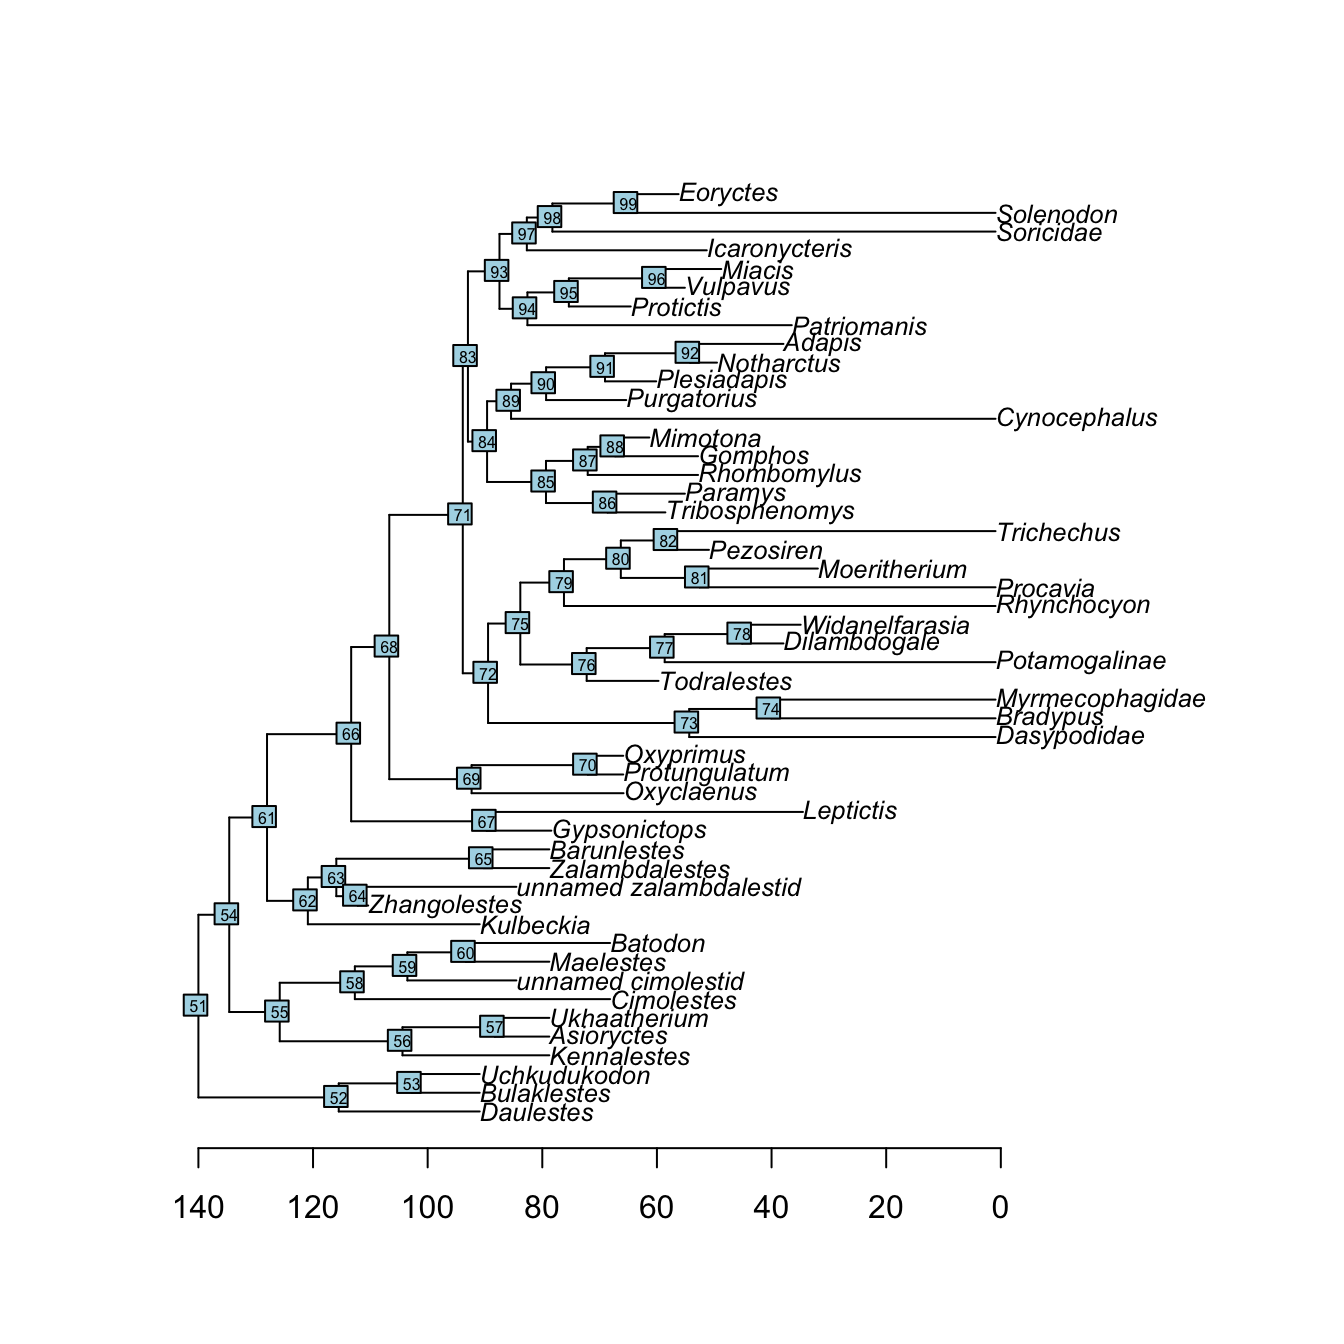
\includegraphics{dispRity_manual_files/figure-latex/unnamed-chunk-10-1.pdf}

Of course you can use your own data as detailed in the
\protect\hyperlink{What-sort-of-data-does-dispRity-work-with}{previous
chapter}.

\subsection{Disparity through time}\label{disparity-through-time}

The \texttt{dispRity.through.time} function calculates disparity through
time, a common analysis in palaeontology. This function (and the
following one) uses an analysis pipeline with a lot of default
parameters to make the analysis as simple as possible. Of course all the
defaults can be changed if required, more on this later.

For a disparity through time analysis, you will need:

\begin{itemize}
\tightlist
\item
  An ordinated matrix (we covered that above)
\item
  A phylogenetic tree: this must be a \texttt{phylo} object (from the
  \texttt{ape} package) and needs a \texttt{root.time} element. To give
  your tree a root time (i.e.~an age for the root), you can simply
  do\textbackslash{}
  \texttt{my\_tree\$root.time\ \textless{}-\ my\_age}.
\item
  The required number of time subsamples (here \texttt{time\ =\ 3})
\item
  Your favourite disparity metric (here the sum of variances)
\end{itemize}

Using the Beck and Lee (2014) data described
\protect\hyperlink{example-data}{above}:

\begin{Shaded}
\begin{Highlighting}[]
\NormalTok{## Measuring disparity through time}
\NormalTok{disparity_data <-}\StringTok{ }\KeywordTok{dispRity.through.time}\NormalTok{(BeckLee_mat50, BeckLee_tree,}
                                        \DataTypeTok{time =} \DecValTok{3}\NormalTok{, }\DataTypeTok{metric =} \KeywordTok{c}\NormalTok{(sum, variances))}
\end{Highlighting}
\end{Shaded}

This generates a \texttt{dispRity} object (see
\protect\hyperlink{guts}{here} for technical details). When displayed,
these \texttt{dispRity} objects provide us with information on the
operations done to the matrix:

\begin{Shaded}
\begin{Highlighting}[]
\NormalTok{## Print the disparity_data object}
\NormalTok{disparity_data}
\end{Highlighting}
\end{Shaded}

\begin{verbatim}
##  ---- dispRity object ---- 
## 3 discrete time subsamples for 50 elements with 48 dimensions:
##     133.51104 - 89.00736, 89.00736 - 44.50368, 44.50368 - 0.
## Data was bootstrapped 100 times (method:"full").
## Disparity was calculated as: metric.
\end{verbatim}

We asked for three subsamples (evenly spread across the age of the
tree), the data was bootstrapped 100 times (default) and the metric used
was the sum of variances.

We can now summarise or plot the \texttt{disparity\_data} object, or
perform statistical tests on it (e.g.~a simple \texttt{lm}):

\begin{Shaded}
\begin{Highlighting}[]
\NormalTok{## Summarising disparity through time}
\KeywordTok{summary}\NormalTok{(disparity_data)}
\end{Highlighting}
\end{Shaded}

\begin{verbatim}
##             subsamples  n   obs bs.median  2.5%   25%   75% 97.5%
## 1 133.51104 - 89.00736  5 1.575     1.305 0.729 1.118 1.420 1.509
## 2  89.00736 - 44.50368 29 1.922     1.867 1.775 1.830 1.889 1.922
## 3         44.50368 - 0 16 1.990     1.871 1.716 1.831 1.914 1.942
\end{verbatim}

\begin{Shaded}
\begin{Highlighting}[]
\NormalTok{## Plotting the results}
\KeywordTok{plot}\NormalTok{(disparity_data, }\DataTypeTok{type =} \StringTok{"continuous"}\NormalTok{)}
\end{Highlighting}
\end{Shaded}

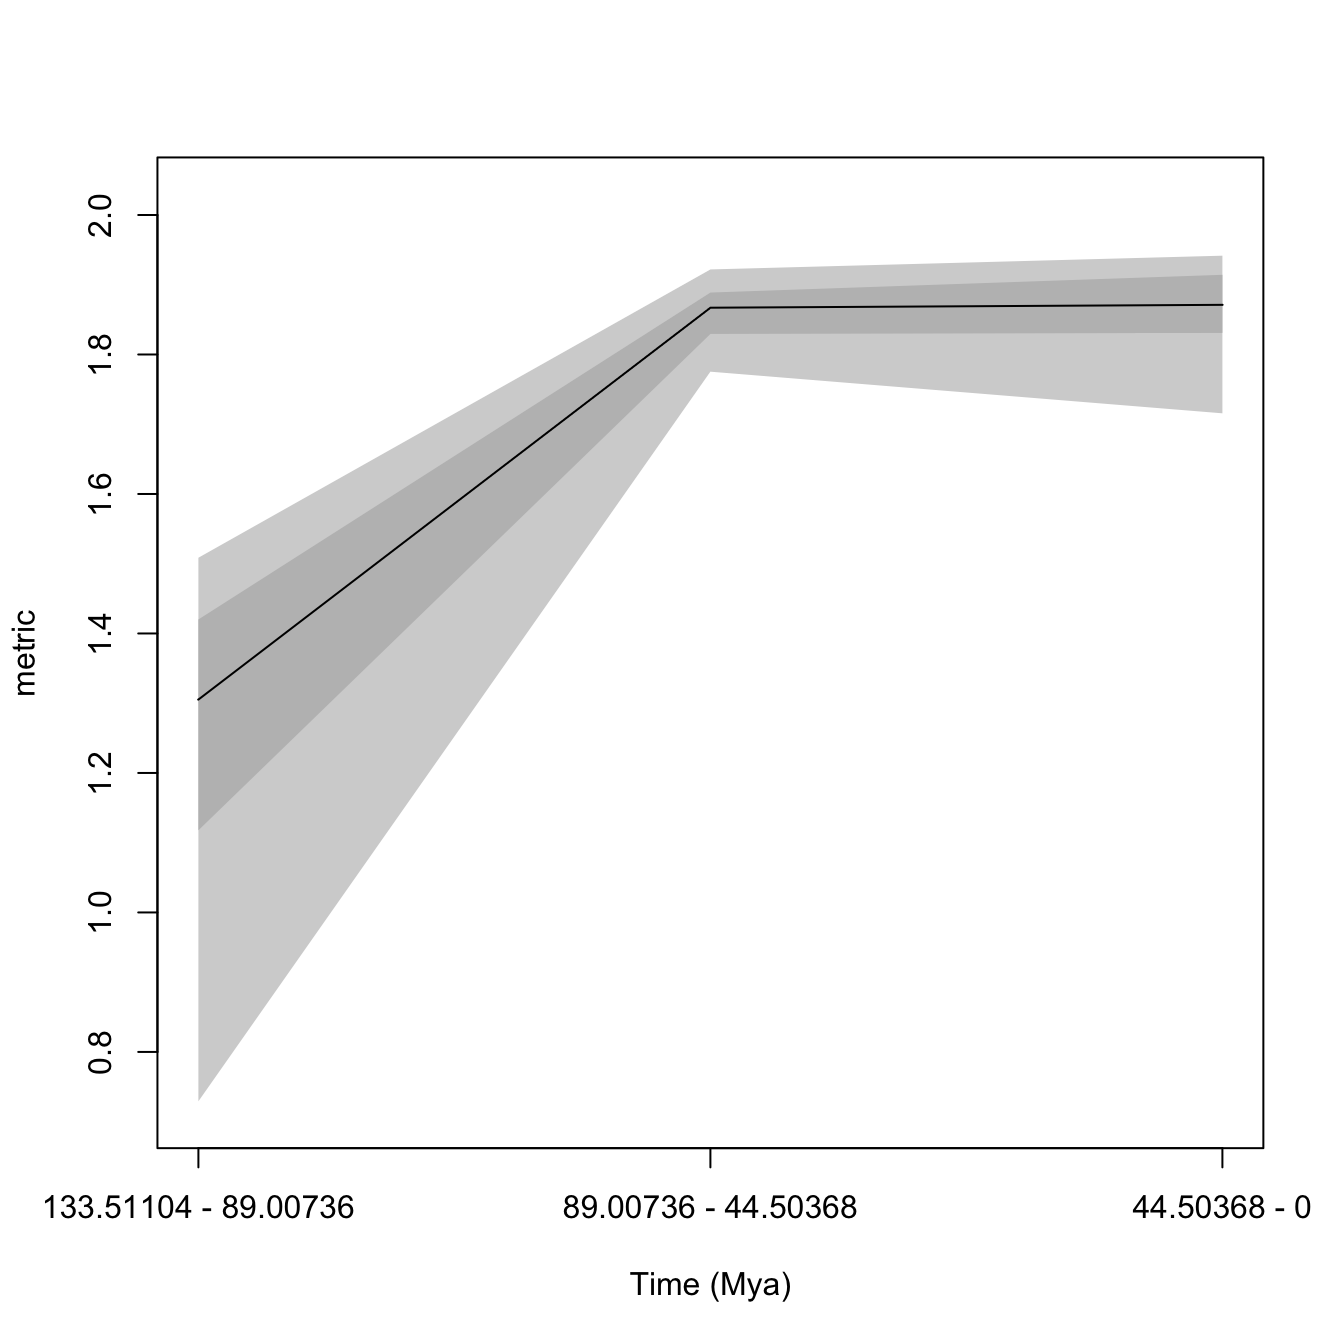
\includegraphics{dispRity_manual_files/figure-latex/unnamed-chunk-13-1.pdf}

\begin{Shaded}
\begin{Highlighting}[]
\NormalTok{## Testing for an difference among the time bins}
\NormalTok{disp_lm <-}\StringTok{ }\KeywordTok{test.dispRity}\NormalTok{(disparity_data, }\DataTypeTok{test =}\NormalTok{ lm, }\DataTypeTok{comparisons =} \StringTok{"all"}\NormalTok{)}
\end{Highlighting}
\end{Shaded}

\begin{verbatim}
## Warning in test.dispRity(disparity_data, test = lm, comparisons = "all"): Multiple p-values will be calculated without adjustment!
## This will inflate Type I error!
\end{verbatim}

\begin{Shaded}
\begin{Highlighting}[]
\KeywordTok{summary}\NormalTok{(disp_lm)}
\end{Highlighting}
\end{Shaded}

\begin{verbatim}
## 
## Call:
## test(formula = data ~ subsamples, data = data)
## 
## Residuals:
##      Min       1Q   Median       3Q      Max 
## -0.56623 -0.04160  0.01049  0.05507  0.31886 
## 
## Coefficients:
##                               Estimate Std. Error t value Pr(>|t|)    
## (Intercept)                    1.25647    0.01270   98.97   <2e-16 ***
## subsamples44.50368 - 0         0.60863    0.01795   33.90   <2e-16 ***
## subsamples89.00736 - 44.50368  0.60169    0.01795   33.51   <2e-16 ***
## ---
## Signif. codes:  0 '***' 0.001 '**' 0.01 '*' 0.05 '.' 0.1 ' ' 1
## 
## Residual standard error: 0.127 on 297 degrees of freedom
## Multiple R-squared:  0.8361, Adjusted R-squared:  0.835 
## F-statistic: 757.5 on 2 and 297 DF,  p-value: < 2.2e-16
\end{verbatim}

Please refer to the \protect\hyperlink{specific-tutorial}{specific
tutorials} for (much!) more information on the nuts and bolts of the
package. You can also directly explore the specific function help files
within R and navigate to related functions.

\hypertarget{disparity-among-groups}{\subsection{Disparity among
groups}\label{disparity-among-groups}}

The \texttt{dispRity.per.group} function is used if you are interested
in looking at disparity among groups rather than through time. For
example, you could ask if there is a difference in disparity between two
groups?

To perform such an analysis, you will need:

\begin{itemize}
\tightlist
\item
  An matrix with rows as elements and columns as dimensions (always!)
\item
  A list of group members: this list should be a list of numeric vectors
  or names corresponding to the row names in the matrix. For example
  \texttt{list("a"\ =\ c(1,2),\ "b"\ =\ c(3,4))} will create a group
  \emph{a} containing elements 1 and 2 from the matrix and a group
  \emph{b} containing elements 3 and 4. Note that elements can be
  present in multiple groups at once.
\item
  Your favourite disparity metric (here the sum of variances)
\end{itemize}

Using the Beck and Lee (2014) data described
\protect\hyperlink{example-data}{above}:

\begin{Shaded}
\begin{Highlighting}[]
\NormalTok{## Creating the two groups (crown versus stem) as a list}
\NormalTok{mammal_groups <-}\StringTok{ }\KeywordTok{list}\NormalTok{(}\StringTok{"crown"}\NormalTok{ =}\StringTok{ }\KeywordTok{c}\NormalTok{(}\DecValTok{16}\NormalTok{, }\DecValTok{19}\OperatorTok{:}\DecValTok{41}\NormalTok{, }\DecValTok{45}\OperatorTok{:}\DecValTok{50}\NormalTok{),}
                      \StringTok{"stem"}\NormalTok{ =}\StringTok{ }\KeywordTok{c}\NormalTok{(}\DecValTok{1}\OperatorTok{:}\DecValTok{15}\NormalTok{, }\DecValTok{17}\OperatorTok{:}\DecValTok{18}\NormalTok{, }\DecValTok{42}\OperatorTok{:}\DecValTok{44}\NormalTok{))}

\NormalTok{## Measuring disparity for each group}
\NormalTok{disparity_data <-}\StringTok{ }\KeywordTok{dispRity.per.group}\NormalTok{(BeckLee_mat50, }\DataTypeTok{group =}\NormalTok{ mammal_groups,}
                                     \DataTypeTok{metric =} \KeywordTok{c}\NormalTok{(sum, variances))}
\end{Highlighting}
\end{Shaded}

We can display the disparity of both groups by simply looking at the
output variable (\texttt{disparity\_data}) and then summarising the
\texttt{disparity\_data} object and plotting it, and/or by performing a
statistical test to compare disparity across the groups (here a Wilcoxon
test).

\begin{Shaded}
\begin{Highlighting}[]
\NormalTok{## Print the disparity_data object}
\NormalTok{disparity_data}
\end{Highlighting}
\end{Shaded}

\begin{verbatim}
##  ---- dispRity object ---- 
## 2 customised subsamples for 50 elements with 48 dimensions:
##     crown, stem.
## Data was bootstrapped 100 times (method:"full").
## Disparity was calculated as: metric.
\end{verbatim}

\begin{Shaded}
\begin{Highlighting}[]
\NormalTok{## Summarising disparity in the different groups}
\KeywordTok{summary}\NormalTok{(disparity_data)}
\end{Highlighting}
\end{Shaded}

\begin{verbatim}
##   subsamples  n   obs bs.median  2.5%   25%   75% 97.5%
## 1      crown 30 1.995     1.936 1.866 1.914 1.947 1.971
## 2       stem 20 1.715     1.632 1.541 1.604 1.667 1.695
\end{verbatim}

\begin{Shaded}
\begin{Highlighting}[]
\NormalTok{## Plotting the results}
\KeywordTok{plot}\NormalTok{(disparity_data)}
\end{Highlighting}
\end{Shaded}

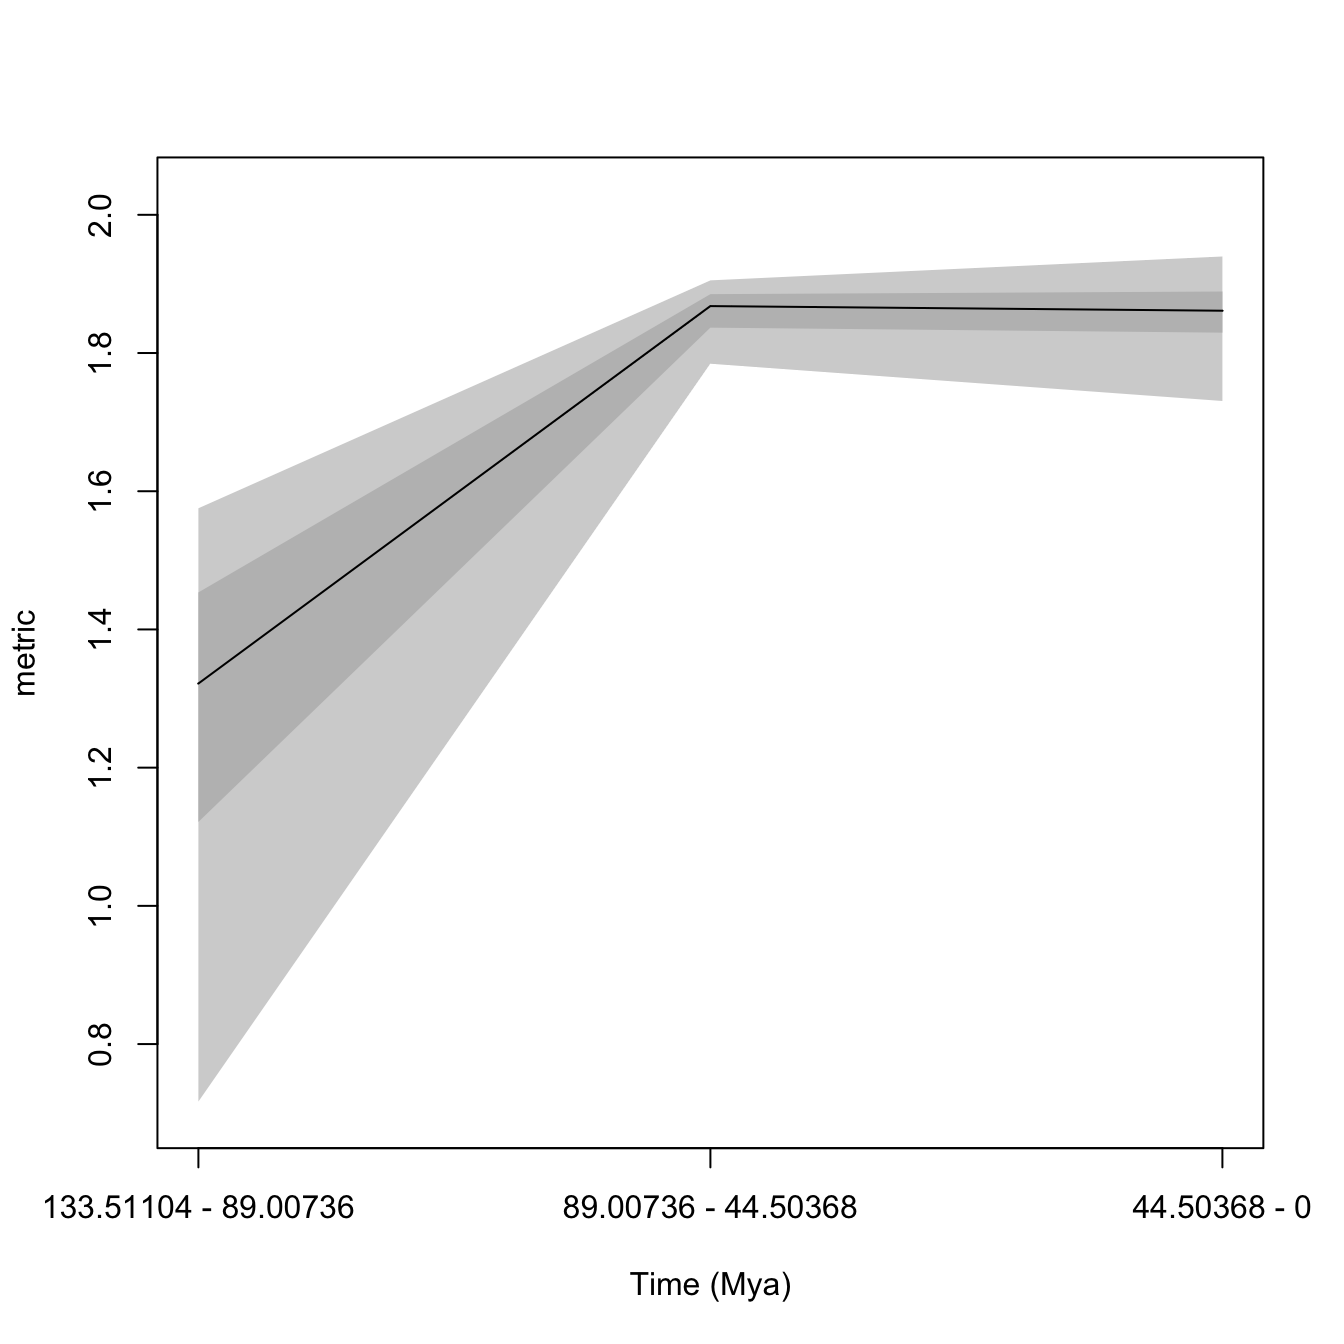
\includegraphics{dispRity_manual_files/figure-latex/unnamed-chunk-15-1.pdf}

\begin{Shaded}
\begin{Highlighting}[]
\NormalTok{## Testing for a difference between the groups}
\KeywordTok{test.dispRity}\NormalTok{(disparity_data, }\DataTypeTok{test =}\NormalTok{ wilcox.test, }\DataTypeTok{details =} \OtherTok{TRUE}\NormalTok{)}
\end{Highlighting}
\end{Shaded}

\begin{verbatim}
## Warning in test.dispRity(disparity_data, test = wilcox.test, details = TRUE): Multiple p-values will be calculated without adjustment!
## This will inflate Type I error!
\end{verbatim}

\begin{verbatim}
## $`crown : stem`
## $`crown : stem`[[1]]
## 
##  Wilcoxon rank sum test with continuity correction
## 
## data:  dots[[1L]][[1L]] and dots[[2L]][[1L]]
## W = 10000, p-value < 2.2e-16
## alternative hypothesis: true location shift is not equal to 0
\end{verbatim}

\chapter{Details of specific
functions}\label{details-of-specific-functions}

The following section contains information specific to some functions.
If any of your questions are not covered in these sections, please refer
to the function help files in R, send me an email
(\href{mailto:guillert@tcd.ie}{\nolinkurl{guillert@tcd.ie}}), or raise
an issue on GitHub. The several tutorials below describe specific
functionalities of certain functions; please always refer to the
function help files for the full function documentation!

Before each section, make sure you loaded the Beck and Lee (2014) data
(see \protect\hyperlink{example-data}{example data} for more details).

\begin{Shaded}
\begin{Highlighting}[]
\NormalTok{## Loading the data}
\KeywordTok{data}\NormalTok{(BeckLee_mat50) ; }\KeywordTok{data}\NormalTok{(BeckLee_mat99)}
\KeywordTok{data}\NormalTok{(BeckLee_tree) ; }\KeywordTok{data}\NormalTok{(BeckLee_ages)}
\end{Highlighting}
\end{Shaded}

\hypertarget{time-slicing}{\section{Time slicing}\label{time-slicing}}

The function \texttt{time.subsamples} allows users to divide the matrix
into different time subsamples or slices given a dated phylogeny that
contains all the elements (i.e.~taxa) from the matrix. Each subsample
generated by this function will then contain all the elements present at
a specific point in time or during a specific period in time.

Two types of time subsamples can be performed by using the
\texttt{method} option:

\begin{itemize}
\tightlist
\item
  Discrete time subsamples (or time-binning) using
  \texttt{method\ =\ discrete}
\item
  Continuous time subsamples (or time-slicing) using
  \texttt{method\ =\ continuous}
\end{itemize}

For the time-slicing method details see Cooper and Guillerme (in prep.).
For both methods, the function takes the \texttt{time} argument which
can be a vector of \texttt{numeric} values for:

\begin{itemize}
\tightlist
\item
  Defining the boundaries of the time bins (when
  \texttt{method\ =\ discrete})
\item
  Defining the time slices (when \texttt{method\ =\ continuous})
\end{itemize}

Otherwise, the \texttt{time} argument can be set as a single
\texttt{numeric} value for automatically generating a given number of
equidistant time-bins/slices. Additionally, it is also possible to input
a dataframe containing the first and last occurrence data (FAD/LAD) for
taxa that span over a longer time than the given tips/nodes age, so taxa
can appear in more than one time bin/slice.

Here is an example for \texttt{method\ =\ discrete}:

\begin{Shaded}
\begin{Highlighting}[]
\NormalTok{## Generating three time bins containing the taxa present every 40 Ma}
\KeywordTok{time.subsamples}\NormalTok{(}\DataTypeTok{data =}\NormalTok{ BeckLee_mat50, }\DataTypeTok{tree =}\NormalTok{ BeckLee_tree, }\DataTypeTok{method =} \StringTok{"discrete"}\NormalTok{,}
                \DataTypeTok{time =} \KeywordTok{c}\NormalTok{(}\DecValTok{120}\NormalTok{, }\DecValTok{80}\NormalTok{, }\DecValTok{40}\NormalTok{, }\DecValTok{0}\NormalTok{))}
\end{Highlighting}
\end{Shaded}

\begin{verbatim}
##  ---- dispRity object ---- 
## 3 discrete time subsamples for 50 elements:
##     120 - 80, 80 - 40, 40 - 0.
\end{verbatim}

Note that we can also generate equivalent results by just telling the
function that we want three time-bins as follow:

\begin{Shaded}
\begin{Highlighting}[]
\NormalTok{## Automatically generate three equal length bins:}
\KeywordTok{time.subsamples}\NormalTok{(}\DataTypeTok{data =}\NormalTok{ BeckLee_mat50, }\DataTypeTok{tree =}\NormalTok{ BeckLee_tree, }\DataTypeTok{method =} \StringTok{"discrete"}\NormalTok{,}
                \DataTypeTok{time =} \DecValTok{3}\NormalTok{)}
\end{Highlighting}
\end{Shaded}

\begin{verbatim}
##  ---- dispRity object ---- 
## 3 discrete time subsamples for 50 elements:
##     133.51104 - 89.00736, 89.00736 - 44.50368, 44.50368 - 0.
\end{verbatim}

In this example, the taxa were split inside each time-bin according to
their age. However, the taxa here are considered as single points in
time. It is totally possible that some taxa could have had longer
longevity and that they exist in multiple time bins. In this case, it is
possible to include them in more than one bin by providing a table of
first and last occurrence dates (FAD/LAD). This table should have the
taxa names as row names and two columns for respectively the first and
last occurrence age:

\begin{Shaded}
\begin{Highlighting}[]
\NormalTok{## Displaying the table of first and last occurrence dates for each taxa}
\KeywordTok{head}\NormalTok{(BeckLee_ages)}
\end{Highlighting}
\end{Shaded}

\begin{verbatim}
##             FAD  LAD
## Adapis     37.2 36.8
## Asioryctes 83.6 72.1
## Leptictis  33.9 33.3
## Miacis     49.0 46.7
## Mimotona   61.6 59.2
## Notharctus 50.2 47.0
\end{verbatim}

\begin{Shaded}
\begin{Highlighting}[]
\NormalTok{## Generating time bins including taxa that might span between them}
\KeywordTok{time.subsamples}\NormalTok{(}\DataTypeTok{data =}\NormalTok{ BeckLee_mat50, }\DataTypeTok{tree =}\NormalTok{ BeckLee_tree, }\DataTypeTok{method =} \StringTok{"discrete"}\NormalTok{,}
                \DataTypeTok{time =} \KeywordTok{c}\NormalTok{(}\DecValTok{120}\NormalTok{, }\DecValTok{80}\NormalTok{, }\DecValTok{40}\NormalTok{, }\DecValTok{0}\NormalTok{), }\DataTypeTok{FADLAD =}\NormalTok{ BeckLee_ages)}
\end{Highlighting}
\end{Shaded}

\begin{verbatim}
##  ---- dispRity object ---- 
## 3 discrete time subsamples for 50 elements:
##     120 - 80, 80 - 40, 40 - 0.
\end{verbatim}

When using this method, the oldest boundary of the first bin (or the
first slice, see below) is automatically generated as the root age plus
1\% of the tree length, as long as at least three elements/taxa are
present at that point in time. The algorithm adds an extra 1\% tree
length until reaching the required minimum of three elements. It is also
possible to include nodes in each bin by using
\texttt{inc.nodes\ =\ TRUE} and providing a matrix that contains the
ordinated distance among tips \emph{and} nodes.

For the time-slicing method (\texttt{method\ =\ continuous}), the idea
is fairly similar. This option, however, requires a matrix that contains
the ordinated distance among taxa \emph{and} nodes and an extra argument
describing the assumed evolutionary model (via the \texttt{model}
argument). This model argument is used when the time slice occurs along
a branch of the tree rather than on a tip or a node, meaning that a
decision must be made about what the value for the branch should be. The
model can be one of the following:

\begin{itemize}
\tightlist
\item
  \texttt{acctran} where the data chosen along the branch is always the
  one of the descendant
\item
  \texttt{deltran} where the data chosen along the branch is always the
  one of the ancestor
\item
  \texttt{punctuated} where the data chosen along the branch is randomly
  chosen between the descendant or the ancestor
\item
  \texttt{gradual} where the data chosen along the branch is either the
  descendant or the ancestor depending on branch length
\end{itemize}

\begin{Shaded}
\begin{Highlighting}[]
\NormalTok{## Generating four time slices every 40 million years under a model of gradual evolution}
\KeywordTok{time.subsamples}\NormalTok{(}\DataTypeTok{data =}\NormalTok{ BeckLee_mat99, }\DataTypeTok{tree =}\NormalTok{ BeckLee_tree, }
    \DataTypeTok{method =} \StringTok{"continuous"}\NormalTok{, }\DataTypeTok{model =} \StringTok{"gradual"}\NormalTok{, }\DataTypeTok{time =} \KeywordTok{c}\NormalTok{(}\DecValTok{120}\NormalTok{, }\DecValTok{80}\NormalTok{, }\DecValTok{40}\NormalTok{, }\DecValTok{0}\NormalTok{),}
    \DataTypeTok{FADLAD =}\NormalTok{ BeckLee_ages)}
\end{Highlighting}
\end{Shaded}

\begin{verbatim}
##  ---- dispRity object ---- 
## 4 continuous (gradual) time subsamples for 99 elements:
##     120, 80, 40, 0.
\end{verbatim}

\begin{Shaded}
\begin{Highlighting}[]
\NormalTok{## Generating four time slices automatically}
\KeywordTok{time.subsamples}\NormalTok{(}\DataTypeTok{data =}\NormalTok{ BeckLee_mat99, }\DataTypeTok{tree =}\NormalTok{ BeckLee_tree,}
    \DataTypeTok{method =} \StringTok{"continuous"}\NormalTok{, }\DataTypeTok{model =} \StringTok{"gradual"}\NormalTok{, }\DataTypeTok{time =} \DecValTok{4}\NormalTok{, }\DataTypeTok{FADLAD =}\NormalTok{ BeckLee_ages)}
\end{Highlighting}
\end{Shaded}

\begin{verbatim}
##  ---- dispRity object ---- 
## 4 continuous (gradual) time subsamples for 99 elements:
##     133.51104, 89.00736, 44.50368, 0.
\end{verbatim}

\hypertarget{customised-subsamples}{\section{Customised
subsamples}\label{customised-subsamples}}

Another way of separating elements into different categories is to use
customised subsamples as briefly explained
\protect\hyperlink{disparity-among-groups}{above}. This function simply
takes the list of elements to put in each group (whether they are the
actual element names or their position in the matrix).

\begin{Shaded}
\begin{Highlighting}[]
\NormalTok{## Creating the two groups as a list}
\NormalTok{mammal_groups <-}\StringTok{ }\KeywordTok{list}\NormalTok{(}\StringTok{"crown"}\NormalTok{ =}\StringTok{ }\KeywordTok{c}\NormalTok{(}\DecValTok{16}\NormalTok{, }\DecValTok{19}\OperatorTok{:}\DecValTok{41}\NormalTok{, }\DecValTok{45}\OperatorTok{:}\DecValTok{50}\NormalTok{),}
                      \StringTok{"stem"}\NormalTok{ =}\StringTok{ }\KeywordTok{c}\NormalTok{(}\DecValTok{1}\OperatorTok{:}\DecValTok{15}\NormalTok{, }\DecValTok{17}\OperatorTok{:}\DecValTok{18}\NormalTok{, }\DecValTok{42}\OperatorTok{:}\DecValTok{44}\NormalTok{))}

\NormalTok{## Separating the dataset into two different groups}
\KeywordTok{custom.subsamples}\NormalTok{(BeckLee_mat50, }\DataTypeTok{group =}\NormalTok{ mammal_groups)}
\end{Highlighting}
\end{Shaded}

\begin{verbatim}
##  ---- dispRity object ---- 
## 2 customised subsamples for 50 elements:
##     crown, stem.
\end{verbatim}

Elements can easily be assigned to different groups if necessary!

\begin{Shaded}
\begin{Highlighting}[]
\NormalTok{## Creating the three groups as a list}
\NormalTok{mammal_groups <-}\StringTok{ }\KeywordTok{list}\NormalTok{(}\StringTok{"crown"}\NormalTok{ =}\StringTok{ }\KeywordTok{c}\NormalTok{(}\DecValTok{16}\NormalTok{, }\DecValTok{19}\OperatorTok{:}\DecValTok{41}\NormalTok{, }\DecValTok{45}\OperatorTok{:}\DecValTok{50}\NormalTok{),}
                      \StringTok{"stem"}\NormalTok{ =}\StringTok{ }\KeywordTok{c}\NormalTok{(}\DecValTok{1}\OperatorTok{:}\DecValTok{15}\NormalTok{, }\DecValTok{17}\OperatorTok{:}\DecValTok{18}\NormalTok{, }\DecValTok{42}\OperatorTok{:}\DecValTok{44}\NormalTok{).}
                      \StringTok{"all"}\NormalTok{ =}\StringTok{ }\KeywordTok{c}\NormalTok{(}\DecValTok{1}\OperatorTok{:}\DecValTok{50}\NormalTok{))}
\end{Highlighting}
\end{Shaded}

\hypertarget{bootstraps-and-rarefactions}{\section{Bootstraps and
rarefactions}\label{bootstraps-and-rarefactions}}

One important step in analysing ordinated matrices is to
pseudo-replicate the data to see how robust the results are, and how
sensitive they are to outliers in the dataset. This can be achieved
using the function \texttt{boot.matrix} to bootstrap and/or rarefy the
data. The default options will bootstrap the matrix 100 times without
rarefaction using the ``full'' bootstrap method (see below):

\begin{Shaded}
\begin{Highlighting}[]
\NormalTok{## Default bootstrapping}
\KeywordTok{boot.matrix}\NormalTok{(}\DataTypeTok{data =}\NormalTok{ BeckLee_mat50)}
\end{Highlighting}
\end{Shaded}

\begin{verbatim}
##  ---- dispRity object ---- 
## 50 elements with 48 dimensions.
## Data was bootstrapped 100 times (method:"full").
\end{verbatim}

The number of bootstrap replicates can be defined using the
\texttt{bootstraps} option. The method can be modified by controlling
which bootstrap algorithm to use through the \texttt{boot.type}
argument. Currently two algorithms are implemented:

\begin{itemize}
\tightlist
\item
  \texttt{full} where the bootstrapping is entirely stochastic (\emph{n}
  elements are replaced by any \emph{m} elements drawn from the data)
\item
  \texttt{single} where only one random element is replaced by one other
  random element for each pseudo-replicate
\end{itemize}

\begin{Shaded}
\begin{Highlighting}[]
\NormalTok{## Bootstrapping with the single bootstrap method}
\KeywordTok{boot.matrix}\NormalTok{(BeckLee_mat50, }\DataTypeTok{boot.type =} \StringTok{"single"}\NormalTok{)}
\end{Highlighting}
\end{Shaded}

\begin{verbatim}
##  ---- dispRity object ---- 
## 50 elements with 48 dimensions.
## Data was bootstrapped 100 times (method:"single").
\end{verbatim}

This function also allows users to rarefy the data using the
\texttt{rarefaction} argument. Rarefaction allows users to limit the
number of elements to be drawn at each bootstrap replication. This is
useful if, for example, one is interested in looking at the effect of
reducing the number of elements on the results of an analysis.

This can be achieved by using the \texttt{rarefaction} option that draws
only \emph{n-x} at each bootstrap replicate (where \emph{x} is the
number of elements not sampled). The default argument is \texttt{FALSE}
but it can be set to \texttt{TRUE} to fully rarefy the data (i.e.~remove
\emph{x} elements for the number of pseudo-replicates, where \emph{x}
varies from the maximum number of elements present in each subsample to
a minimum of three elements). It can also be set to one or more
\texttt{numeric} values to only rarefy to the corresponding number of
elements.

\begin{Shaded}
\begin{Highlighting}[]
\NormalTok{## Bootstrapping with the full rarefaction}
\KeywordTok{boot.matrix}\NormalTok{(BeckLee_mat50, }\DataTypeTok{bootstraps =} \DecValTok{20}\NormalTok{, }\DataTypeTok{rarefaction =} \OtherTok{TRUE}\NormalTok{)}
\end{Highlighting}
\end{Shaded}

\begin{verbatim}
##  ---- dispRity object ---- 
## 50 elements with 48 dimensions.
## Data was bootstrapped 20 times (method:"full") and fully rarefied.
\end{verbatim}

\begin{Shaded}
\begin{Highlighting}[]
\NormalTok{## Or with a set number of rarefaction levels}
\KeywordTok{boot.matrix}\NormalTok{(BeckLee_mat50, }\DataTypeTok{bootstraps =} \DecValTok{20}\NormalTok{, }\DataTypeTok{rarefaction =} \KeywordTok{c}\NormalTok{(}\DecValTok{6}\OperatorTok{:}\DecValTok{8}\NormalTok{, }\DecValTok{3}\NormalTok{))}
\end{Highlighting}
\end{Shaded}

\begin{verbatim}
##  ---- dispRity object ---- 
## 50 elements with 48 dimensions.
## Data was bootstrapped 20 times (method:"full") and rarefied to 6, 7, 8, 3 elements.
\end{verbatim}

One additional important argument is \texttt{dimensions} that specifies
how many dimensions from the matrix should be used for further analysis.
When missing, all dimensions from the ordinated matrix are used.

\begin{Shaded}
\begin{Highlighting}[]
\NormalTok{## Using the first 50% of the dimensions}
\KeywordTok{boot.matrix}\NormalTok{(BeckLee_mat50, }\DataTypeTok{dimensions =} \FloatTok{0.5}\NormalTok{)}
\end{Highlighting}
\end{Shaded}

\begin{verbatim}
##  ---- dispRity object ---- 
## 50 elements with 24 dimensions.
## Data was bootstrapped 100 times (method:"full").
\end{verbatim}

\begin{Shaded}
\begin{Highlighting}[]
\NormalTok{## Using the first 10 dimensions}
\KeywordTok{boot.matrix}\NormalTok{(BeckLee_mat50, }\DataTypeTok{dimensions =} \DecValTok{10}\NormalTok{)}
\end{Highlighting}
\end{Shaded}

\begin{verbatim}
##  ---- dispRity object ---- 
## 50 elements with 10 dimensions.
## Data was bootstrapped 100 times (method:"full").
\end{verbatim}

Of course, one could directly supply the subsamples generated above
(using \texttt{time.subsamples} or \texttt{custom.subsamples}) to this
function.

\begin{Shaded}
\begin{Highlighting}[]
\NormalTok{## Creating subsamples of crown and stem mammals}
\NormalTok{crown_stem <-}\StringTok{ }\KeywordTok{custom.subsamples}\NormalTok{(BeckLee_mat50,}
                                \DataTypeTok{group =} \KeywordTok{list}\NormalTok{(}\StringTok{"crown"}\NormalTok{ =}\StringTok{ }\KeywordTok{c}\NormalTok{(}\DecValTok{16}\NormalTok{, }\DecValTok{19}\OperatorTok{:}\DecValTok{41}\NormalTok{, }\DecValTok{45}\OperatorTok{:}\DecValTok{50}\NormalTok{), }
                                             \StringTok{"stem"}\NormalTok{ =}\StringTok{ }\KeywordTok{c}\NormalTok{(}\DecValTok{1}\OperatorTok{:}\DecValTok{15}\NormalTok{, }\DecValTok{17}\OperatorTok{:}\DecValTok{18}\NormalTok{, }\DecValTok{42}\OperatorTok{:}\DecValTok{44}\NormalTok{)))}
\NormalTok{## Bootstrapping and rarefying these groups}
\KeywordTok{boot.matrix}\NormalTok{(crown_stem, }\DataTypeTok{bootstraps =} \DecValTok{200}\NormalTok{, }\DataTypeTok{rarefaction =} \OtherTok{TRUE}\NormalTok{)}
\end{Highlighting}
\end{Shaded}

\begin{verbatim}
##  ---- dispRity object ---- 
## 2 customised subsamples for 50 elements with 48 dimensions:
##     crown, stem.
## Data was bootstrapped 200 times (method:"full") and fully rarefied.
\end{verbatim}

\begin{Shaded}
\begin{Highlighting}[]
\NormalTok{## Creating time slice subsamples}
\NormalTok{time_slices <-}\StringTok{ }\KeywordTok{time.subsamples}\NormalTok{(}\DataTypeTok{data =}\NormalTok{ BeckLee_mat99, }\DataTypeTok{tree =}\NormalTok{ BeckLee_tree, }
                               \DataTypeTok{method =} \StringTok{"continuous"}\NormalTok{, }\DataTypeTok{model =} \StringTok{"gradual"}\NormalTok{, }
                               \DataTypeTok{time =} \KeywordTok{c}\NormalTok{(}\DecValTok{120}\NormalTok{, }\DecValTok{80}\NormalTok{, }\DecValTok{40}\NormalTok{, }\DecValTok{0}\NormalTok{),}
                               \DataTypeTok{FADLAD =}\NormalTok{ BeckLee_ages)}

\NormalTok{## Bootstrapping the time slice subsamples}
\KeywordTok{boot.matrix}\NormalTok{(time_slices, }\DataTypeTok{bootstraps =} \DecValTok{100}\NormalTok{)}
\end{Highlighting}
\end{Shaded}

\begin{verbatim}
##  ---- dispRity object ---- 
## 4 continuous (gradual) time subsamples for 99 elements with 97 dimensions:
##     120, 80, 40, 0.
## Data was bootstrapped 100 times (method:"full").
\end{verbatim}

\hypertarget{disparity-metrics}{\section{Disparity
metrics}\label{disparity-metrics}}

There are many ways of measuring disparity! In brief, disparity is a
summary metric that will represent an aspect of an ordinated space
(e.g.~a MDS, PCA, PCO, PCoA). For example, one can look at ellipsoid
hyper-volume of the ordinated space (Donohue \emph{et al.} 2013), the
sum and the product of the ranges and variances (Wills \emph{et al.}
1994) or the median position of the elements relative to their centroid
(Wills \emph{et al.} 1994). Of course, there are many more examples of
metrics one can use for describing some aspect of the ordinated space,
with some performing better than other ones at particular descriptive
tasks, and some being more generalist.

Because of this great diversity of metrics, the package
\texttt{dispRity} does not have one way to measure disparity but rather
proposes to facilitate users in defining their own disparity metric that
will best suit their particular analysis. In fact, the core function of
the package, \texttt{dispRity}, allows the user to define any metric
with the \texttt{metric} argument. However the \texttt{metric} argument
has to follow certain rules:

\begin{enumerate}
\def\labelenumi{\arabic{enumi}.}
\tightlist
\item
  It must be composed from one to three \texttt{function} objects;
\item
  The function(s) must take as a first argument a \texttt{matrix} or a
  \texttt{vector};
\item
  The function(s) must be of one of the three dimension-levels described
  below;
\item
  At least one of the functions must be of dimension-level 1 or 2 (see
  below).
\end{enumerate}

\subsection{The function
dimension-levels}\label{the-function-dimension-levels}

The metric function dimension-levels determine the ``dimensionality of
decomposition'' of the input matrix. In other words, each
dimension-level designates the dimensions of the output, i.e.~either
three (a \texttt{matrix}); two (a \texttt{vector}); or one (a single
\texttt{numeric} value) dimension.

\begin{figure}
\centering
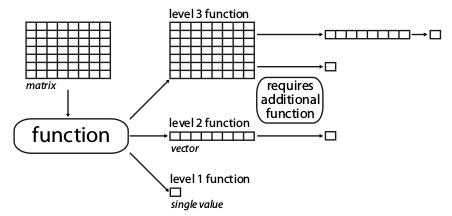
\includegraphics{dispRity_fun.png}
\caption{Illustration of the different dimension-levels of functions
with an input \texttt{matrix}}
\end{figure}

\subsubsection{Dimension-level 1
functions}\label{dimension-level-1-functions}

A dimension-level 1 function will decompose a \texttt{matrix} or a
\texttt{vector} into a single value:

\begin{Shaded}
\begin{Highlighting}[]
\NormalTok{## Creating a dummy matrix}
\NormalTok{dummy_matrix <-}\StringTok{ }\KeywordTok{matrix}\NormalTok{(}\KeywordTok{rnorm}\NormalTok{(}\DecValTok{12}\NormalTok{), }\DecValTok{4}\NormalTok{, }\DecValTok{3}\NormalTok{)}

\NormalTok{## Example of dimension-level 1 functions}
\KeywordTok{mean}\NormalTok{(dummy_matrix)}
\end{Highlighting}
\end{Shaded}

\begin{verbatim}
## [1] -0.3227241
\end{verbatim}

\begin{Shaded}
\begin{Highlighting}[]
\KeywordTok{median}\NormalTok{(dummy_matrix)}
\end{Highlighting}
\end{Shaded}

\begin{verbatim}
## [1] -0.2690165
\end{verbatim}

Any summary metric such as mean or median are good examples of
dimension-level 1 functions as they reduce the matrix to a single
dimension (i.e.~one value).

\subsubsection{Dimension-level 2
functions}\label{dimension-level-2-functions}

A dimension-level 2 function will decompose a \texttt{matrix} into a
\texttt{vector}.

\begin{Shaded}
\begin{Highlighting}[]
\NormalTok{## Defining the function as the product of rows}
\NormalTok{prod.rows <-}\StringTok{ }\ControlFlowTok{function}\NormalTok{(matrix) }\KeywordTok{apply}\NormalTok{(matrix, }\DecValTok{1}\NormalTok{, prod)}

\NormalTok{## A dimension-level 2 metric}
\KeywordTok{prod.rows}\NormalTok{(dummy_matrix)}
\end{Highlighting}
\end{Shaded}

\begin{verbatim}
## [1] -1.2630799  0.2148864 -0.1797556 -0.2421790
\end{verbatim}

Several dimension-level 2 functions are implemented in \texttt{dispRity}
(see \texttt{?dispRity.metric}) such as the \texttt{variances} or
\texttt{ranges} functions that calculate the variance or the range of
each dimension of the ordinated matrix respectively.

\subsubsection{Dimension-level 3
functions}\label{dimension-level-3-functions}

Finally a dimension-level 3 function will transform the matrix into
another matrix. Note that the dimension of the output matrix doesn't
need to match the the input matrix:

\begin{Shaded}
\begin{Highlighting}[]
\NormalTok{## A dimension-level 3 metric}
\KeywordTok{var}\NormalTok{(dummy_matrix)}
\end{Highlighting}
\end{Shaded}

\begin{verbatim}
##          [,1]      [,2]      [,3]
## [1,] 1.916420 1.9501955 0.2907060
## [2,] 1.950196 3.2948635 0.3958234
## [3,] 0.290706 0.3958234 0.6704976
\end{verbatim}

\begin{Shaded}
\begin{Highlighting}[]
\NormalTok{## A dimension-level 3 metric with a forced matrix output}
\KeywordTok{as.matrix}\NormalTok{(}\KeywordTok{dist}\NormalTok{(dummy_matrix))}
\end{Highlighting}
\end{Shaded}

\begin{verbatim}
##          1        2        3        4
## 1 0.000000 5.140790 4.005068 3.120827
## 2 5.140790 0.000000 2.179318 2.982267
## 3 4.005068 2.179318 0.000000 2.174896
## 4 3.120827 2.982267 2.174896 0.000000
\end{verbatim}

\subsection{\texorpdfstring{\texttt{make.metric}}{make.metric}}\label{make.metric}

Of course, functions can be more complex and involve multiple operations
such as the \texttt{centroids} function (see \texttt{?dispRity.metric})
that calculates the Euclidean distance between each element and the
centroid of the ordinated space. The \texttt{make.metric} function
implemented in \texttt{dispRity} is designed to help test and find the
dimension-level of the functions. This function tests:

\begin{enumerate}
\def\labelenumi{\arabic{enumi}.}
\tightlist
\item
  If your function can deal with a \texttt{matrix} or a \texttt{vector}
  as an input;
\item
  Your function's dimension-level according to its output
  (dimension-level 1, 2 or 3, see above);
\item
  Whether the function can be implemented in the \texttt{dispRity}
  function (the function is fed into a \texttt{lapply} loop).
\end{enumerate}

For example, let's see if the functions described above are the right
dimension-levels:

\begin{Shaded}
\begin{Highlighting}[]
\NormalTok{## Which dimension-level is the mean function? And can it be used in dispRity?}
\KeywordTok{make.metric}\NormalTok{(mean)}
\end{Highlighting}
\end{Shaded}

\begin{verbatim}
## mean outputs a single value.
## mean is detected as being a dimension-level 1 function.
\end{verbatim}

\begin{Shaded}
\begin{Highlighting}[]
\NormalTok{## Which dimension-level is the prod.rows function? And can it be used in dispRity?}
\KeywordTok{make.metric}\NormalTok{(prod.rows)}
\end{Highlighting}
\end{Shaded}

\begin{verbatim}
## prod.rows outputs a matrix object.
## prod.rows is detected as being a dimension-level 2 function.
\end{verbatim}

\begin{Shaded}
\begin{Highlighting}[]
\NormalTok{## Which dimension-level is the var function? And can it be used in dispRity?}
\KeywordTok{make.metric}\NormalTok{(var)}
\end{Highlighting}
\end{Shaded}

\begin{verbatim}
## var outputs a matrix object.
## var is detected as being a dimension-level 3 function.
## Additional dimension-level 2 and/or 1 function(s) will be needed.
\end{verbatim}

A non verbose version of the function is also available. This can be
done using the option \texttt{silent\ =\ TRUE} and will simply output
the dimension-level of the metric.

\begin{Shaded}
\begin{Highlighting}[]
\NormalTok{## Testing whether mean is dimension-level 1}
\ControlFlowTok{if}\NormalTok{(}\KeywordTok{make.metric}\NormalTok{(mean, }\DataTypeTok{silent =} \OtherTok{TRUE}\NormalTok{) }\OperatorTok{!=}\StringTok{ "level1"}\NormalTok{) \{}
    \KeywordTok{message}\NormalTok{(}\StringTok{"The metric is not dimension-level 1."}\NormalTok{)}
\NormalTok{\}}
\NormalTok{## Testing whether var is dimension-level 1}
\ControlFlowTok{if}\NormalTok{(}\KeywordTok{make.metric}\NormalTok{(var, }\DataTypeTok{silent =} \OtherTok{TRUE}\NormalTok{) }\OperatorTok{!=}\StringTok{ "level1"}\NormalTok{) \{}
    \KeywordTok{message}\NormalTok{(}\StringTok{"The metric is not dimension-level 1."}\NormalTok{)}
\NormalTok{\}}
\end{Highlighting}
\end{Shaded}

\begin{verbatim}
## The metric is not dimension-level 1.
\end{verbatim}

\subsection{\texorpdfstring{Metrics in the \texttt{dispRity}
function}{Metrics in the dispRity function}}\label{metrics-in-the-disprity-function}

Using this metric structure, we can easily use any disparity metric in
the \texttt{dispRity} function as follows:

\begin{Shaded}
\begin{Highlighting}[]
\NormalTok{## Measuring disparity as the standard deviation of all the values of the}
\NormalTok{## ordinated matrix (dimension-level 1 function).}
\KeywordTok{summary}\NormalTok{(}\KeywordTok{dispRity}\NormalTok{(BeckLee_mat50, }\DataTypeTok{metric =}\NormalTok{ sd))}
\end{Highlighting}
\end{Shaded}

\begin{verbatim}
##   subsamples  n   obs
## 1          1 50 0.201
\end{verbatim}

\begin{Shaded}
\begin{Highlighting}[]
\NormalTok{## Measuring disparity as the standard deviation of the variance of each axis of}
\NormalTok{## the ordinated matrix (dimension-level 1 and 2 functions).}
\KeywordTok{summary}\NormalTok{(}\KeywordTok{dispRity}\NormalTok{(BeckLee_mat50, }\DataTypeTok{metric =} \KeywordTok{c}\NormalTok{(sd, variances)))}
\end{Highlighting}
\end{Shaded}

\begin{verbatim}
##   subsamples  n   obs
## 1          1 50 0.028
\end{verbatim}

\begin{Shaded}
\begin{Highlighting}[]
\NormalTok{## Measuring disparity as the standard deviation of the variance of each axis of}
\NormalTok{## the variance covariance matrix (dimension-level 1, 2 and 3 functions).}
\KeywordTok{summary}\NormalTok{(}\KeywordTok{dispRity}\NormalTok{(BeckLee_mat50, }\DataTypeTok{metric =} \KeywordTok{c}\NormalTok{(sd, variances, var)), }\DataTypeTok{round =} \DecValTok{10}\NormalTok{)}
\end{Highlighting}
\end{Shaded}

\begin{verbatim}
##   subsamples  n          obs
## 1          1 50 0.0001025857
\end{verbatim}

Note that the order of each function in the metric argument does not
matter, the \texttt{dispRity} function will automatically detect the
function dimension-levels (using \texttt{make.metric}) and apply them to
the data in decreasing order (dimension-level 3 \textgreater{} 2
\textgreater{} 1).

\begin{Shaded}
\begin{Highlighting}[]
\NormalTok{## Disparity as the standard deviation of the variance of each axis of the}
\NormalTok{## variance covariance matrix:}
\NormalTok{disparity1 <-}\StringTok{ }\KeywordTok{summary}\NormalTok{(}\KeywordTok{dispRity}\NormalTok{(BeckLee_mat50, }\DataTypeTok{metric =} \KeywordTok{c}\NormalTok{(sd, variances, var)),}
                      \DataTypeTok{round =} \DecValTok{10}\NormalTok{)}

\NormalTok{## Same as above but using a different function order for the metric argument}
\NormalTok{disparity2 <-}\StringTok{ }\KeywordTok{summary}\NormalTok{(}\KeywordTok{dispRity}\NormalTok{(BeckLee_mat50, }\DataTypeTok{metric =} \KeywordTok{c}\NormalTok{(variances, sd, var)),}
                      \DataTypeTok{round =} \DecValTok{10}\NormalTok{)}

\NormalTok{## Both ways output the same disparity values:}
\NormalTok{disparity1 }\OperatorTok{==}\StringTok{ }\NormalTok{disparity2}
\end{Highlighting}
\end{Shaded}

\begin{verbatim}
##      subsamples    n  obs
## [1,]       TRUE TRUE TRUE
\end{verbatim}

In these examples, we considered disparity to be a single value. For
example, in the previous example, we defined disparity as the standard
deviation of the variances of each column of the variance/covariance
matrix (\texttt{metric\ =\ c(variances,\ sd,\ var)}). It is, however,
possible to calculate
\protect\hyperlink{disparity-as-a-distribution}{disparity as a
distribution}.

\subsection{\texorpdfstring{Metrics implemented in
\texttt{dispRity}}{Metrics implemented in dispRity}}\label{metrics-implemented-in-disprity}

Several disparity metrics are implemented in the \texttt{dispRity}
package. The detailed list can be found in \texttt{?dispRity.metric}
along with some description of each metric.

\begin{longtable}[]{@{}llll@{}}
\toprule
\begin{minipage}[b]{0.08\columnwidth}\raggedright\strut
Level\strut
\end{minipage} & \begin{minipage}[b]{0.08\columnwidth}\raggedright\strut
Name\strut
\end{minipage} & \begin{minipage}[b]{0.61\columnwidth}\raggedright\strut
Description\strut
\end{minipage} & \begin{minipage}[b]{0.11\columnwidth}\raggedright\strut
Source\strut
\end{minipage}\tabularnewline
\midrule
\endhead
\begin{minipage}[t]{0.08\columnwidth}\raggedright\strut
1\strut
\end{minipage} & \begin{minipage}[t]{0.08\columnwidth}\raggedright\strut
\texttt{ellipse.volume}1\strut
\end{minipage} & \begin{minipage}[t]{0.61\columnwidth}\raggedright\strut
The volume of the ellipsoid of the space\strut
\end{minipage} & \begin{minipage}[t]{0.11\columnwidth}\raggedright\strut
Donohue \emph{et al.} (2013)\strut
\end{minipage}\tabularnewline
\begin{minipage}[t]{0.08\columnwidth}\raggedright\strut
1\strut
\end{minipage} & \begin{minipage}[t]{0.08\columnwidth}\raggedright\strut
\texttt{convhull.surface}\strut
\end{minipage} & \begin{minipage}[t]{0.61\columnwidth}\raggedright\strut
The surface of the convex hull formed by all the elements\strut
\end{minipage} & \begin{minipage}[t]{0.11\columnwidth}\raggedright\strut
\href{https://cran.r-project.org/web/packages/geometry/index.html}{\texttt{geometry}}\texttt{::convhulln}\strut
\end{minipage}\tabularnewline
\begin{minipage}[t]{0.08\columnwidth}\raggedright\strut
1\strut
\end{minipage} & \begin{minipage}[t]{0.08\columnwidth}\raggedright\strut
\texttt{convhull.volume}\strut
\end{minipage} & \begin{minipage}[t]{0.61\columnwidth}\raggedright\strut
The volume of the convex hull formed by all the elements\strut
\end{minipage} & \begin{minipage}[t]{0.11\columnwidth}\raggedright\strut
\href{https://cran.r-project.org/web/packages/geometry/index.html}{\texttt{geometry}}\texttt{::convhulln}\strut
\end{minipage}\tabularnewline
\bottomrule
\end{longtable}

1 \textbar{} \texttt{diagonal} \textbar{} The longest distance in the
ordinated space (like the diagonal in two dimensions) \textbar{}
\texttt{dispRity} \textbar{} 2 \textbar{} \texttt{ranges} \textbar{} The
range of each dimension \textbar{} \texttt{dispRity} \textbar{} 2
\textbar{} \texttt{variances} \textbar{} The variance of each dimension
\textbar{} \texttt{dispRity} \textbar{} 2 \textbar{} \texttt{centroids}2
\textbar{} The distance between each element and the centroid of the
ordinated space \textbar{} \texttt{dispRity} \textbar{} 1 \textbar{}
\texttt{mode.val} \textbar{} The modal value \textbar{}
\texttt{dispRity} \textbar{}

1: This function uses an estimation of the eigenvalue that only works
for MDS or PCoA ordinations (not PCA).

2: Note that by default, the centroid is the centroid of the elements.
It can, however, be fixed to a different value by using the
\texttt{centroid} argument
\texttt{centroids(space,\ centroid\ =\ rep(0,\ ncol(space)))}, for
example the origin of the ordinated space.

\subsection{Equations and
implementations}\label{equations-and-implementations}

Some of the functions described below are implemented in the
\texttt{dispRity} package and do not require any other packages to
calculate
(\href{https://github.com/TGuillerme/dispRity/blob/master/R/dispRity.metric.R}{see
implementation here}).

\begin{equation}
    ellipse.volume = \frac{\pi^{k/2}}{\Gamma(\frac{k}{2}+1)}\displaystyle\prod_{i=1}^{k} (\lambda_{i}^{0.5})
\end{equation}

Where \emph{k} is the number of dimensions, and \(\lambda_i\) is the
eigenvalue of each dimension.

\begin{equation}
    diagonal = \sqrt{\sum_{i=1}^{k}|max(k_i) - min(k_i)|}
\end{equation}

Where \emph{k} is the number of dimensions.

\begin{equation}
    ranges = |max(k_i) - min(k_i)|
\end{equation}

Where \emph{k} is the number of dimensions.

\begin{equation}
    variances = \sigma^{2}{k_i}
\end{equation}

Where \emph{k} is the number of dimensions, and \(\sigma^{2}\) is their
variance.

\begin{equation}
    centroids = \sqrt{\sum_{i=1}^{n}{({k}_{n}-Centroid_{k})^2}}
\end{equation}

Where \emph{n} is each element in the ordinated space, \emph{k} is the
number of dimensions, and \(Centroid_{k}\) is their mean (or can be set
to another value).

\subsection{Using the different disparity
metrics}\label{using-the-different-disparity-metrics}

Here is a brief demonstration of the main metrics implemented in
\texttt{dispRity}. First, we will create a dummy/simulated ordinated
space using the \texttt{space.maker} utility function (more about that
\protect\hyperlink{space.maker}{here}:

\begin{Shaded}
\begin{Highlighting}[]
\NormalTok{## Creating a 10*5 normal space}
\KeywordTok{set.seed}\NormalTok{(}\DecValTok{1}\NormalTok{)}
\NormalTok{dummy_space <-}\StringTok{ }\KeywordTok{space.maker}\NormalTok{(}\DecValTok{10}\NormalTok{, }\DecValTok{5}\NormalTok{, rnorm)}
\end{Highlighting}
\end{Shaded}

We will use this simulated space to demonstrate the different metrics.

\subsubsection{Volumes and surface
metrics}\label{volumes-and-surface-metrics}

The functions \texttt{ellipse.volume}, \texttt{convhull.surface} and
\texttt{convhull.volume} all measure the surface or the volume of the
ordinated space occupied:

\begin{Shaded}
\begin{Highlighting}[]
\NormalTok{## Calculating the ellipsoid volume}
\KeywordTok{summary}\NormalTok{(}\KeywordTok{dispRity}\NormalTok{(dummy_space, }\DataTypeTok{metric =}\NormalTok{ ellipse.volume))}
\end{Highlighting}
\end{Shaded}

\begin{verbatim}
##   subsamples  n   obs
## 1          1 10 257.8
\end{verbatim}

\begin{quote}
Because there is only one subsample (i.e.~one matrix) in the dispRity
object, this operation is the equivalent of
\texttt{ellipse.volume(dummy\_space)} (with rounding).
\end{quote}

\begin{Shaded}
\begin{Highlighting}[]
\NormalTok{## Calculating the convex hull surface}
\KeywordTok{summary}\NormalTok{(}\KeywordTok{dispRity}\NormalTok{(dummy_space, }\DataTypeTok{metric =}\NormalTok{ convhull.surface))}
\end{Highlighting}
\end{Shaded}

\begin{verbatim}
##   subsamples  n   obs
## 1          1 10 11.91
\end{verbatim}

\begin{Shaded}
\begin{Highlighting}[]
\NormalTok{## Calculating the convex hull volume}
\KeywordTok{summary}\NormalTok{(}\KeywordTok{dispRity}\NormalTok{(dummy_space, }\DataTypeTok{metric =}\NormalTok{ convhull.volume))}
\end{Highlighting}
\end{Shaded}

\begin{verbatim}
##   subsamples  n   obs
## 1          1 10 1.031
\end{verbatim}

The convex hull functions make a (good) estimation of the
multidimensional properties of the ordinated space.

\begin{quote}
Cautionary note: measuring volumes in a high number of dimensions can be
strongly affected by the
\href{https://en.wikipedia.org/wiki/Curse_of_dimensionality}{curse of
dimensionality} that often results in near 0 disparity values.
\end{quote}

\subsubsection{Ranges, variances and
diagonal}\label{ranges-variances-and-diagonal}

The functions \texttt{ranges}, \texttt{variances} and \texttt{diagonal}
all measure properties of the ordinated space based on its dimensional
properties (they are also less affected by the ``curse of
dimensionality''):

\texttt{ranges} and \texttt{variances} both work on the same principle
and measure the range/variance of each dimension:

\begin{Shaded}
\begin{Highlighting}[]
\NormalTok{## Calculating the ranges of each dimension in the ordinated space}
\KeywordTok{ranges}\NormalTok{(dummy_space)}
\end{Highlighting}
\end{Shaded}

\begin{verbatim}
## [1] 2.430909 3.726481 2.908329 2.735739 1.588603
\end{verbatim}

\begin{Shaded}
\begin{Highlighting}[]
\NormalTok{## Calculating disparity as the distribution of these ranges}
\KeywordTok{summary}\NormalTok{(}\KeywordTok{dispRity}\NormalTok{(dummy_space, }\DataTypeTok{metric =}\NormalTok{ ranges))}
\end{Highlighting}
\end{Shaded}

\begin{verbatim}
##   subsamples  n obs.median  2.5%   25%   75% 97.5%
## 1          1 10      2.736 1.673 2.431 2.908 3.645
\end{verbatim}

\begin{Shaded}
\begin{Highlighting}[]
\NormalTok{## Calculating disparity as the sum and the product of these ranges}
\KeywordTok{summary}\NormalTok{(}\KeywordTok{dispRity}\NormalTok{(dummy_space, }\DataTypeTok{metric =} \KeywordTok{c}\NormalTok{(sum, ranges)))}
\end{Highlighting}
\end{Shaded}

\begin{verbatim}
##   subsamples  n   obs
## 1          1 10 13.39
\end{verbatim}

\begin{Shaded}
\begin{Highlighting}[]
\KeywordTok{summary}\NormalTok{(}\KeywordTok{dispRity}\NormalTok{(dummy_space, }\DataTypeTok{metric =} \KeywordTok{c}\NormalTok{(prod, ranges)))}
\end{Highlighting}
\end{Shaded}

\begin{verbatim}
##   subsamples  n   obs
## 1          1 10 114.5
\end{verbatim}

\begin{Shaded}
\begin{Highlighting}[]
\NormalTok{## Calculating the variances of each dimension in the ordinated space}
\KeywordTok{variances}\NormalTok{(dummy_space)}
\end{Highlighting}
\end{Shaded}

\begin{verbatim}
## [1] 0.6093144 1.1438620 0.9131859 0.6537768 0.3549372
\end{verbatim}

\begin{Shaded}
\begin{Highlighting}[]
\NormalTok{## Calculating disparity as the distribution of these variances}
\KeywordTok{summary}\NormalTok{(}\KeywordTok{dispRity}\NormalTok{(dummy_space, }\DataTypeTok{metric =}\NormalTok{ variances))}
\end{Highlighting}
\end{Shaded}

\begin{verbatim}
##   subsamples  n obs.median 2.5%   25%   75% 97.5%
## 1          1 10      0.654 0.38 0.609 0.913 1.121
\end{verbatim}

\begin{Shaded}
\begin{Highlighting}[]
\NormalTok{## Calculating disparity as the sum and the product of these variances}
\KeywordTok{summary}\NormalTok{(}\KeywordTok{dispRity}\NormalTok{(dummy_space, }\DataTypeTok{metric =} \KeywordTok{c}\NormalTok{(sum, variances)))}
\end{Highlighting}
\end{Shaded}

\begin{verbatim}
##   subsamples  n   obs
## 1          1 10 3.675
\end{verbatim}

\begin{Shaded}
\begin{Highlighting}[]
\KeywordTok{summary}\NormalTok{(}\KeywordTok{dispRity}\NormalTok{(dummy_space, }\DataTypeTok{metric =} \KeywordTok{c}\NormalTok{(prod, variances)))}
\end{Highlighting}
\end{Shaded}

\begin{verbatim}
##   subsamples  n   obs
## 1          1 10 0.148
\end{verbatim}

The \texttt{diagonal} function measures the multidimensional diagonal of
the whole space (i.e.~in our case the longest Euclidean distance in our
five dimensional space):

\begin{Shaded}
\begin{Highlighting}[]
\NormalTok{## Calculating the ordinated space's diagonal}
\KeywordTok{summary}\NormalTok{(}\KeywordTok{dispRity}\NormalTok{(dummy_space, }\DataTypeTok{metric =}\NormalTok{ diagonal))}
\end{Highlighting}
\end{Shaded}

\begin{verbatim}
##   subsamples  n   obs
## 1          1 10 3.659
\end{verbatim}

\begin{quote}
This metric is only a Euclidean diagonal (mathematically valid) if the
dimensions within the space are all orthogonal!
\end{quote}

\subsubsection{Centroids metric}\label{centroids-metric}

The \texttt{centroids} metric allows users to measure the position of
the different elements compared to a fixed point in the ordinated space.
By default, this function measures the distance between each element and
their centroid (centre point):

\begin{Shaded}
\begin{Highlighting}[]
\NormalTok{## The distribution of the distances between each element and their centroid}
\KeywordTok{summary}\NormalTok{(}\KeywordTok{dispRity}\NormalTok{(dummy_space, }\DataTypeTok{metric =}\NormalTok{ centroids))}
\end{Highlighting}
\end{Shaded}

\begin{verbatim}
##   subsamples  n obs.median  2.5%   25%   75% 97.5%
## 1          1 10      1.435 0.788 1.267 1.993 3.167
\end{verbatim}

\begin{Shaded}
\begin{Highlighting}[]
\NormalTok{## Disparity as the median value of these distances}
\KeywordTok{summary}\NormalTok{(}\KeywordTok{dispRity}\NormalTok{(dummy_space, }\DataTypeTok{metric =} \KeywordTok{c}\NormalTok{(median, centroids)))}
\end{Highlighting}
\end{Shaded}

\begin{verbatim}
##   subsamples  n   obs
## 1          1 10 1.435
\end{verbatim}

It is however possible to fix the coordinates of the centroid to a
specific point in the ordinated space, as long as it has the correct
number of dimensions:

\begin{Shaded}
\begin{Highlighting}[]
\NormalTok{## The distance between each element and the origin of the ordinated space}
\KeywordTok{summary}\NormalTok{(}\KeywordTok{dispRity}\NormalTok{(dummy_space, }\DataTypeTok{metric =}\NormalTok{ centroids, }\DataTypeTok{centroid =} \KeywordTok{c}\NormalTok{(}\DecValTok{0}\NormalTok{,}\DecValTok{0}\NormalTok{,}\DecValTok{0}\NormalTok{,}\DecValTok{0}\NormalTok{,}\DecValTok{0}\NormalTok{)))}
\end{Highlighting}
\end{Shaded}

\begin{verbatim}
##   subsamples  n obs.median  2.5% 25%   75% 97.5%
## 1          1 10      1.487 0.785 1.2 2.044 3.176
\end{verbatim}

\begin{Shaded}
\begin{Highlighting}[]
\NormalTok{## Disparity as the distance between each element and a specific point in space}
\KeywordTok{summary}\NormalTok{(}\KeywordTok{dispRity}\NormalTok{(dummy_space, }\DataTypeTok{metric =}\NormalTok{ centroids, }\DataTypeTok{centroid =} \KeywordTok{c}\NormalTok{(}\DecValTok{0}\NormalTok{,}\DecValTok{1}\NormalTok{,}\DecValTok{2}\NormalTok{,}\DecValTok{3}\NormalTok{,}\DecValTok{4}\NormalTok{)))}
\end{Highlighting}
\end{Shaded}

\begin{verbatim}
##   subsamples  n obs.median  2.5%   25%   75% 97.5%
## 1          1 10      5.489 4.293 5.032 6.155 6.957
\end{verbatim}

\section{Summarising dispRity data
(plots)}\label{summarising-disprity-data-plots}

Because of its architecture, printing \texttt{dispRity} objects only
summarises their content but does not print the disparity value measured
or associated analysis (more about this
\protect\hyperlink{manipulating-dispRity-objects}{here}). To actually
see what is in a dispRity object, one can either use the
\texttt{summary} function for visualising the data in a table or
\texttt{plot} to have a graphical representation of the results.

\subsection{\texorpdfstring{Summarising \texttt{dispRity}
data}{Summarising dispRity data}}\label{summarising-disprity-data}

This function is an S3 function (\texttt{summary.dispRity}) allowing
users to summarise the content of \texttt{dispRity} objects that contain
disparity calculations.

\begin{Shaded}
\begin{Highlighting}[]
\NormalTok{## Example data from previous sections}
\NormalTok{crown_stem <-}\StringTok{ }\KeywordTok{custom.subsamples}\NormalTok{(BeckLee_mat50,}
                                \DataTypeTok{group =} \KeywordTok{list}\NormalTok{(}\StringTok{"crown"}\NormalTok{ =}\StringTok{ }\KeywordTok{c}\NormalTok{(}\DecValTok{16}\NormalTok{, }\DecValTok{19}\OperatorTok{:}\DecValTok{41}\NormalTok{, }\DecValTok{45}\OperatorTok{:}\DecValTok{50}\NormalTok{), }
                                             \StringTok{"stem"}\NormalTok{ =}\StringTok{ }\KeywordTok{c}\NormalTok{(}\DecValTok{1}\OperatorTok{:}\DecValTok{15}\NormalTok{, }\DecValTok{17}\OperatorTok{:}\DecValTok{18}\NormalTok{, }\DecValTok{42}\OperatorTok{:}\DecValTok{44}\NormalTok{)))}
\NormalTok{## Bootstrapping and rarefying these groups}
\NormalTok{boot_crown_stem <-}\StringTok{ }\KeywordTok{boot.matrix}\NormalTok{(crown_stem, }\DataTypeTok{bootstraps =} \DecValTok{100}\NormalTok{, }\DataTypeTok{rarefaction =} \OtherTok{TRUE}\NormalTok{)}
\NormalTok{## Calculate disparity}
\NormalTok{disparity_crown_stem <-}\StringTok{ }\KeywordTok{dispRity}\NormalTok{(boot_crown_stem, }\DataTypeTok{metric =} \KeywordTok{c}\NormalTok{(sum, variances))}

\NormalTok{## Creating time slice subsamples}
\NormalTok{time_slices <-}\StringTok{ }\KeywordTok{time.subsamples}\NormalTok{(}\DataTypeTok{data =}\NormalTok{ BeckLee_mat99, }\DataTypeTok{tree =}\NormalTok{ BeckLee_tree, }
    \DataTypeTok{method =} \StringTok{"continuous"}\NormalTok{, }\DataTypeTok{model =} \StringTok{"gradual"}\NormalTok{, }\DataTypeTok{time =} \KeywordTok{c}\NormalTok{(}\DecValTok{120}\NormalTok{, }\DecValTok{80}\NormalTok{, }\DecValTok{40}\NormalTok{, }\DecValTok{0}\NormalTok{),}
    \DataTypeTok{FADLAD =}\NormalTok{ BeckLee_ages)}
\NormalTok{## Bootstrapping the time slice subsamples}
\NormalTok{boot_time_slices <-}\StringTok{ }\KeywordTok{boot.matrix}\NormalTok{(time_slices, }\DataTypeTok{bootstraps =} \DecValTok{100}\NormalTok{)}
\NormalTok{## Calculate disparity}
\NormalTok{disparity_time_slices <-}\StringTok{ }\KeywordTok{dispRity}\NormalTok{(boot_time_slices, }\DataTypeTok{metric =} \KeywordTok{c}\NormalTok{(sum, variances))}

\NormalTok{## Creating time bin subsamples}
\NormalTok{time_bins <-}\StringTok{ }\KeywordTok{time.subsamples}\NormalTok{(}\DataTypeTok{data =}\NormalTok{ BeckLee_mat99, }\DataTypeTok{tree =}\NormalTok{ BeckLee_tree, }
    \DataTypeTok{method =} \StringTok{"discrete"}\NormalTok{, }\DataTypeTok{time =} \KeywordTok{c}\NormalTok{(}\DecValTok{120}\NormalTok{, }\DecValTok{80}\NormalTok{, }\DecValTok{40}\NormalTok{, }\DecValTok{0}\NormalTok{), }\DataTypeTok{FADLAD =}\NormalTok{ BeckLee_ages,}
    \DataTypeTok{inc.nodes =} \OtherTok{TRUE}\NormalTok{)}
\NormalTok{## Bootstrapping the time bin subsamples}
\NormalTok{boot_time_bins <-}\StringTok{ }\KeywordTok{boot.matrix}\NormalTok{(time_bins, }\DataTypeTok{bootstraps =} \DecValTok{100}\NormalTok{)}
\NormalTok{## Calculate disparity}
\NormalTok{disparity_time_bins <-}\StringTok{ }\KeywordTok{dispRity}\NormalTok{(boot_time_bins, }\DataTypeTok{metric =} \KeywordTok{c}\NormalTok{(sum, variances))}
\end{Highlighting}
\end{Shaded}

These objects are easy to summarise as follows:

\begin{Shaded}
\begin{Highlighting}[]
\NormalTok{## Default summary}
\KeywordTok{summary}\NormalTok{(disparity_time_slices)}
\end{Highlighting}
\end{Shaded}

\begin{verbatim}
##   subsamples  n   obs bs.median  2.5%   25%   75% 97.5%
## 1        120  5 2.823     2.341 1.376 1.964 2.582 2.823
## 2         80 19 3.233     3.064 2.790 2.957 3.152 3.224
## 3         40 15 3.421     3.197 2.771 3.034 3.313 3.506
## 4          0 10 4.055     3.664 3.282 3.565 3.788 3.924
\end{verbatim}

Information about the number of elements in each subsample and the
observed (i.e.~non-bootstrapped) disparity are also calculated. This is
specifically handy when rarefying the data for example:

\begin{Shaded}
\begin{Highlighting}[]
\KeywordTok{head}\NormalTok{(}\KeywordTok{summary}\NormalTok{(disparity_crown_stem))}
\end{Highlighting}
\end{Shaded}

\begin{verbatim}
##   subsamples  n   obs bs.median  2.5%   25%   75% 97.5%
## 1      crown 30 1.995     1.930 1.866 1.909 1.950 1.970
## 2      crown 29    NA     1.932 1.871 1.915 1.953 1.974
## 3      crown 28    NA     1.926 1.852 1.903 1.942 1.978
## 4      crown 27    NA     1.935 1.860 1.908 1.954 1.982
## 5      crown 26    NA     1.931 1.859 1.908 1.953 1.977
## 6      crown 25    NA     1.933 1.855 1.909 1.954 1.978
\end{verbatim}

The summary functions can also take various options such as:

\begin{itemize}
\tightlist
\item
  \texttt{quantile} values for the confidence interval levels (by
  default, the 50 and 95 quantiles are calculated)
\item
  \texttt{cent.tend} for the central tendency to use for summarising the
  results (default is \texttt{median})
\item
  rounding\texttt{option\ corresponding\ to\ the\ number\ of\ decimal\ places\ to\ print\ (default\ is}2`)
\item
  \texttt{recall} option for printing the call of the \texttt{dispRity}
  object as well (default is \texttt{FALSE})
\end{itemize}

These options can easily be changed from the defaults as follows:

\begin{Shaded}
\begin{Highlighting}[]
\NormalTok{## Same as above but using the 88th quantile and the standard deviation as the summary }
\KeywordTok{summary}\NormalTok{(disparity_time_slices, }\DataTypeTok{quantile =} \DecValTok{88}\NormalTok{, }\DataTypeTok{cent.tend =}\NormalTok{ sd)}
\end{Highlighting}
\end{Shaded}

\begin{verbatim}
##   subsamples  n   obs bs.sd    6%   94%
## 1        120  5 2.823 0.404 1.658 2.672
## 2         80 19 3.233 0.121 2.841 3.203
## 3         40 15 3.421 0.201 2.886 3.452
## 4          0 10 4.055 0.176 3.423 3.889
\end{verbatim}

\begin{Shaded}
\begin{Highlighting}[]
\NormalTok{## Printing the details of the object and rounding the values to the 5th decimal place}
\KeywordTok{summary}\NormalTok{(disparity_time_slices, }\DataTypeTok{recall =} \OtherTok{TRUE}\NormalTok{, }\DataTypeTok{rounding =} \DecValTok{5}\NormalTok{)}
\end{Highlighting}
\end{Shaded}

\begin{verbatim}
##  ---- dispRity object ---- 
## 4 continuous (gradual) time subsamples for 99 elements with 97 dimensions:
##     120, 80, 40, 0.
## Data was bootstrapped 100 times (method:"full").
## Disparity was calculated as: c(sum, variances).
\end{verbatim}

\begin{verbatim}
##   subsamples  n     obs bs.median    2.5%     25%     75%   97.5%
## 1        120  5 2.82292   2.34070 1.37637 1.96358 2.58235 2.82292
## 2         80 19 3.23312   3.06388 2.78953 2.95651 3.15168 3.22359
## 3         40 15 3.42091   3.19699 2.77094 3.03428 3.31260 3.50645
## 4          0 10 4.05457   3.66433 3.28211 3.56532 3.78844 3.92372
\end{verbatim}

Note that the summary table is a \texttt{data.frame}, hence it is as
easy to modify as any dataframe using \texttt{dplyr}. You can also
export it in \texttt{csv} format using \texttt{write.csv} or
\texttt{write\_csv} or even directly export into \texttt{LaTeX} format
using the following;

\begin{Shaded}
\begin{Highlighting}[]
\NormalTok{## Loading the xtable package}
\KeywordTok{require}\NormalTok{(xtable)}
\NormalTok{## Converting the table in LaTeX}
\KeywordTok{xtable}\NormalTok{(}\KeywordTok{summary}\NormalTok{(disparity_time_slices))}
\end{Highlighting}
\end{Shaded}

\subsection{\texorpdfstring{Plotting \texttt{dispRity}
data}{Plotting dispRity data}}\label{plotting-disprity-data}

An alternative (and more fun!) way to display the calculated disparity
is to plot the results using the S3 method \texttt{plot.dispRity}. This
function takes the same options as \texttt{summary.dispRity} along with
various graphical options described in the function help files (see
\texttt{?plot.dispRity}).

The plots can be of four different types:

\begin{itemize}
\tightlist
\item
  \texttt{continuous} for displaying continuous disparity curves
\item
  \texttt{box}, \texttt{lines}, and \texttt{polygons} to display
  discrete disparity results in respectively a boxplot, confidence
  interval lines, and confidence interval polygons.
\end{itemize}

\begin{quote}
This argument can be left empty. In this case, the algorithm will
automatically detect the type of subsamples from the \texttt{dispRity}
object and plot accordingly.
\end{quote}

It is also possible to display the number of elements in each subsample
(as a horizontal dotted line) using the option
\texttt{elements\ =\ TRUE}. Additionally, when the data is rarefied, one
can indicate which level of rarefaction to display (i.e.~only display
the results for a certain number of elements) by using the
\texttt{rarefaction} argument.

\begin{Shaded}
\begin{Highlighting}[]
\NormalTok{## Graphical parameters}
\NormalTok{op <-}\StringTok{ }\KeywordTok{par}\NormalTok{(}\DataTypeTok{mfrow =} \KeywordTok{c}\NormalTok{(}\DecValTok{2}\NormalTok{, }\DecValTok{2}\NormalTok{), }\DataTypeTok{bty =} \StringTok{"n"}\NormalTok{)}

\NormalTok{## Plotting continuous disparity results}
\KeywordTok{plot}\NormalTok{(disparity_time_slices, }\DataTypeTok{type =} \StringTok{"continuous"}\NormalTok{)}

\NormalTok{## Plotting discrete disparity results}
\KeywordTok{plot}\NormalTok{(disparity_crown_stem, }\DataTypeTok{type =} \StringTok{"box"}\NormalTok{)}

\NormalTok{## As above but using lines for the rarefaction level of 20 elements only}
\KeywordTok{plot}\NormalTok{(disparity_crown_stem, }\DataTypeTok{type =} \StringTok{"line"}\NormalTok{, }\DataTypeTok{rarefaction =} \DecValTok{20}\NormalTok{)}

\NormalTok{## As above but using polygons while also displaying the number of elements}
\KeywordTok{plot}\NormalTok{(disparity_crown_stem, }\DataTypeTok{type =} \StringTok{"polygon"}\NormalTok{, }\DataTypeTok{elements =} \OtherTok{TRUE}\NormalTok{)}
\end{Highlighting}
\end{Shaded}

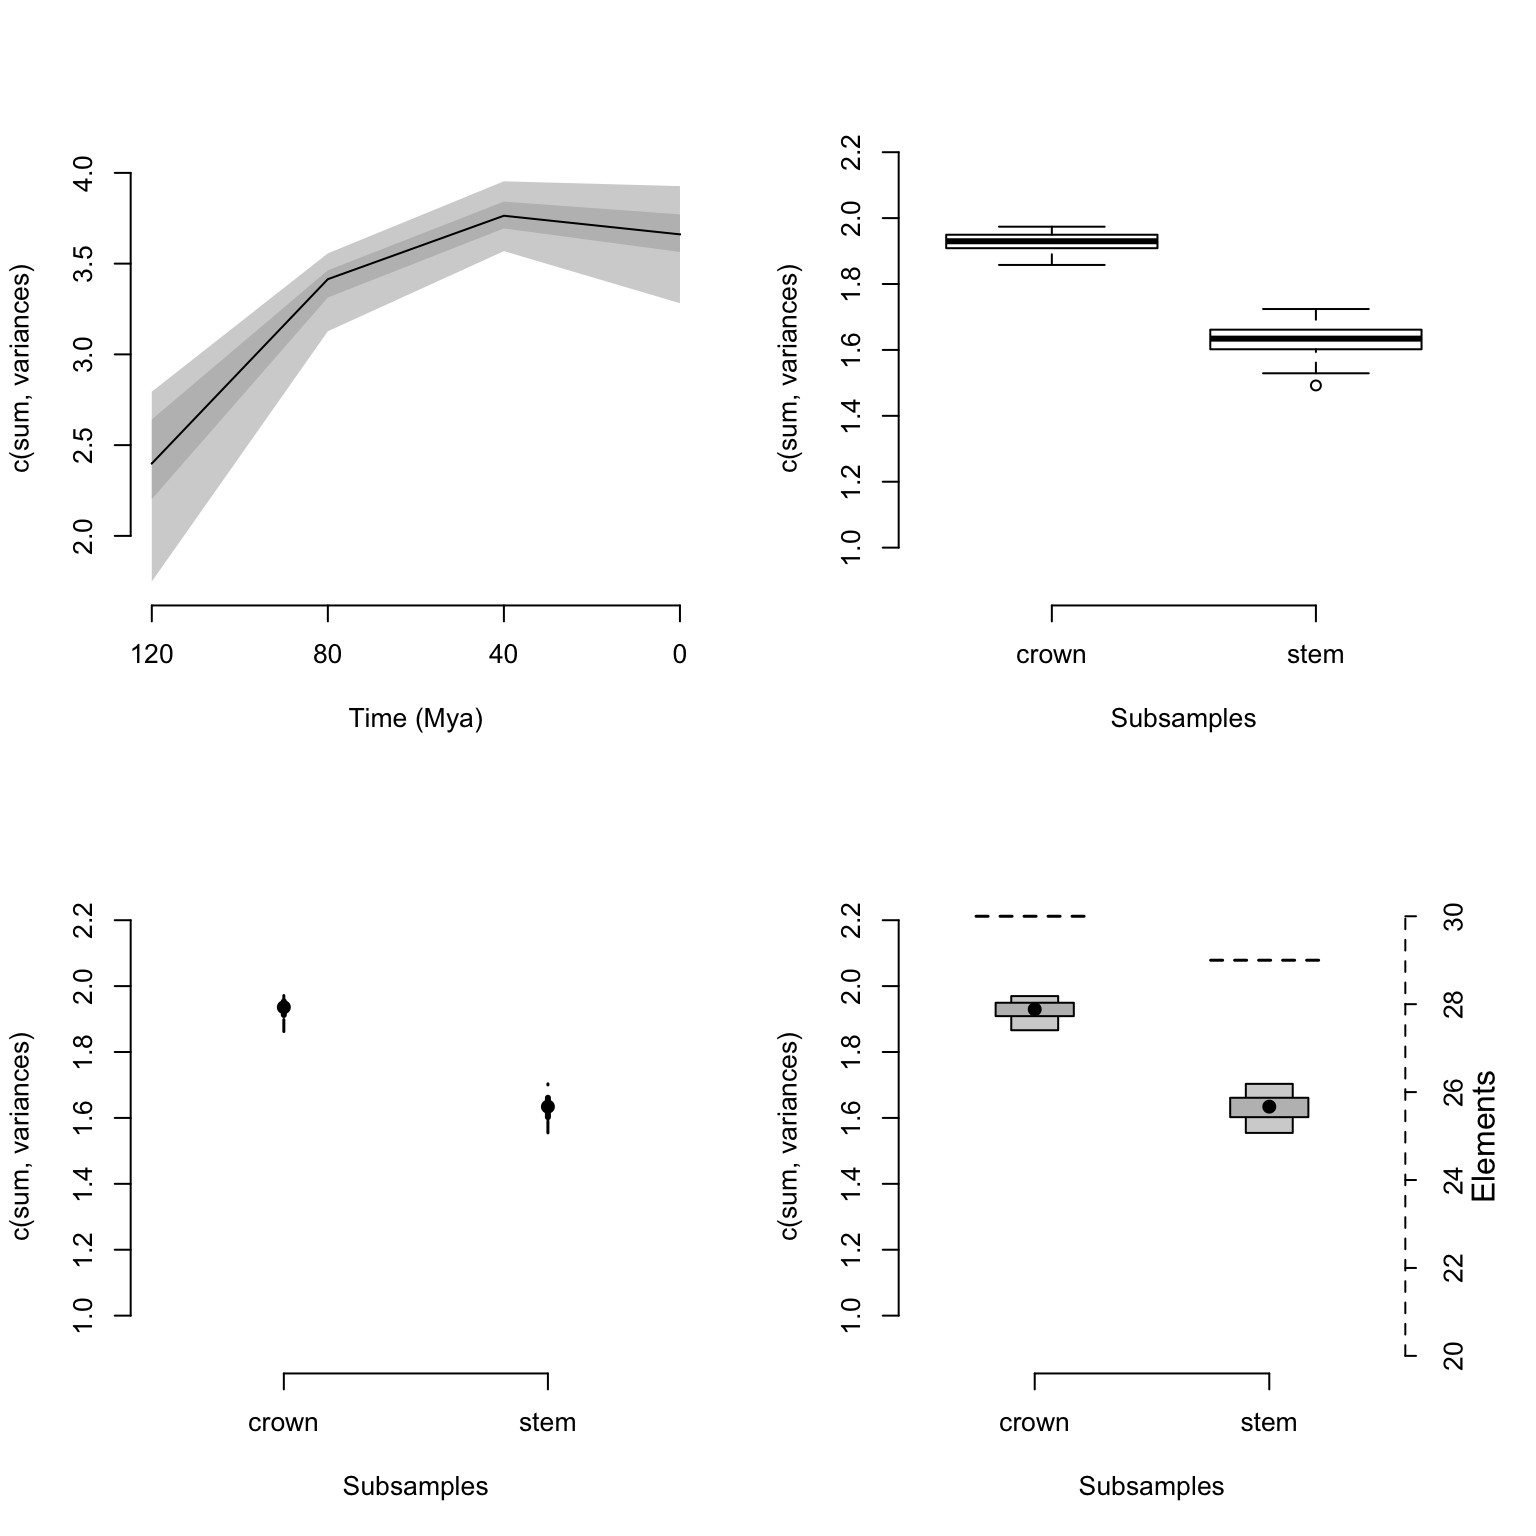
\includegraphics{dispRity_manual_files/figure-latex/unnamed-chunk-47-1.pdf}

\begin{Shaded}
\begin{Highlighting}[]
\NormalTok{## Resetting graphical parameters}
\KeywordTok{par}\NormalTok{(op)}
\end{Highlighting}
\end{Shaded}

Since \texttt{plot.dispRity} uses the arguments from the generic
\texttt{plot} method, it is of course possible to change pretty much
everything using the regular plot arguments:

\begin{Shaded}
\begin{Highlighting}[]
\NormalTok{## Graphical options}
\NormalTok{op <-}\StringTok{ }\KeywordTok{par}\NormalTok{(}\DataTypeTok{bty =} \StringTok{"n"}\NormalTok{)}

\NormalTok{## Plotting the results with some classic options from plot}
\KeywordTok{plot}\NormalTok{(disparity_time_slices, }\DataTypeTok{col =} \KeywordTok{c}\NormalTok{(}\StringTok{"blue"}\NormalTok{, }\StringTok{"orange"}\NormalTok{, }\StringTok{"green"}\NormalTok{),}
    \DataTypeTok{ylab =} \KeywordTok{c}\NormalTok{(}\StringTok{"Some measurement"}\NormalTok{), }\DataTypeTok{xlab =} \StringTok{"Some other measurement"}\NormalTok{,}
    \DataTypeTok{main =} \StringTok{"Many options..."}\NormalTok{, }\DataTypeTok{ylim =} \KeywordTok{c}\NormalTok{(}\DecValTok{5}\NormalTok{, }\DecValTok{0}\NormalTok{), }\DataTypeTok{xlim =} \KeywordTok{c}\NormalTok{(}\DecValTok{4}\NormalTok{, }\DecValTok{0}\NormalTok{))}

\NormalTok{## Adding a legend}
\KeywordTok{legend}\NormalTok{(}\StringTok{"topleft"}\NormalTok{, }\DataTypeTok{legend =} \KeywordTok{c}\NormalTok{(}\StringTok{"Central tendency"}\NormalTok{,}
                             \StringTok{"Confidence interval 1"}\NormalTok{,}
                            \StringTok{"Confidence interval 2"}\NormalTok{),}
      \DataTypeTok{col =} \KeywordTok{c}\NormalTok{(}\StringTok{"blue"}\NormalTok{, }\StringTok{"orange"}\NormalTok{, }\StringTok{"green"}\NormalTok{), }\DataTypeTok{pch =} \DecValTok{19}\NormalTok{)}
\end{Highlighting}
\end{Shaded}

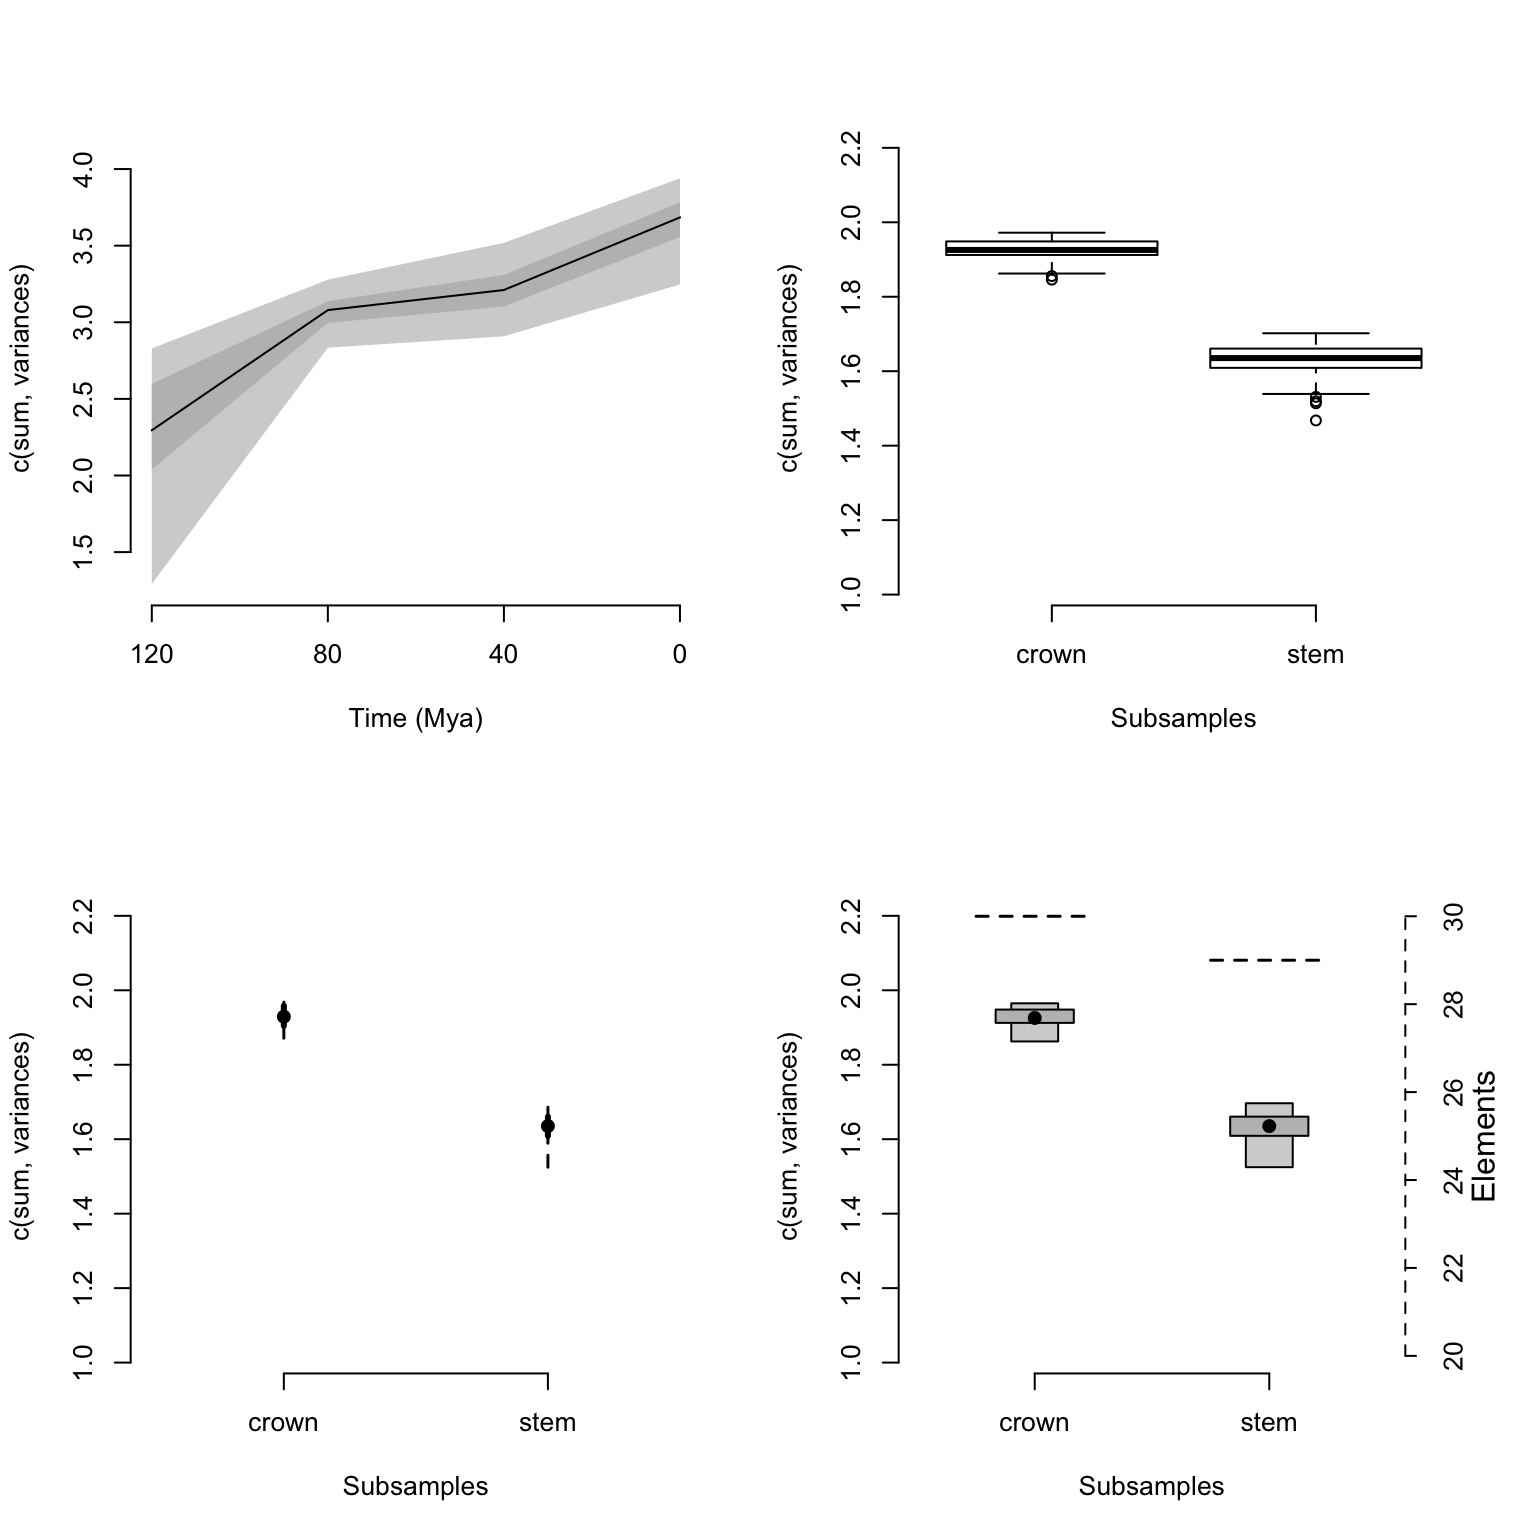
\includegraphics{dispRity_manual_files/figure-latex/unnamed-chunk-48-1.pdf}

\begin{Shaded}
\begin{Highlighting}[]
\NormalTok{## Resetting graphical parameters}
\KeywordTok{par}\NormalTok{(op)}
\end{Highlighting}
\end{Shaded}

In addition to the classic \texttt{plot} arguments, the function can
also take arguments that are specific to \texttt{plot.dispRity} like
adding the number of elements or rarefaction level (as described above),
and also changing the values of the quantiles to plot as well as the
central tendency.

\begin{Shaded}
\begin{Highlighting}[]
\NormalTok{## Graphical options}
\NormalTok{op <-}\StringTok{ }\KeywordTok{par}\NormalTok{(}\DataTypeTok{bty =} \StringTok{"n"}\NormalTok{)}

\NormalTok{## Plotting the results with some plot.dispRity arguments}
\KeywordTok{plot}\NormalTok{(disparity_time_slices, }\DataTypeTok{quantile =} \KeywordTok{c}\NormalTok{(}\KeywordTok{seq}\NormalTok{(}\DataTypeTok{from =} \DecValTok{10}\NormalTok{, }\DataTypeTok{to =} \DecValTok{100}\NormalTok{, }\DataTypeTok{by =} \DecValTok{10}\NormalTok{)),}
    \DataTypeTok{cent.tend =}\NormalTok{ sd, }\DataTypeTok{type =} \StringTok{"c"}\NormalTok{, }\DataTypeTok{elements =} \OtherTok{TRUE}\NormalTok{, }\DataTypeTok{col =} \KeywordTok{c}\NormalTok{(}\StringTok{"black"}\NormalTok{, }\KeywordTok{rainbow}\NormalTok{(}\DecValTok{10}\NormalTok{)),}
    \DataTypeTok{ylab =} \KeywordTok{c}\NormalTok{(}\StringTok{"Disparity"}\NormalTok{, }\StringTok{"Diversity"}\NormalTok{), }\DataTypeTok{time.subsamples =} \OtherTok{FALSE}\NormalTok{,}
    \DataTypeTok{xlab =} \StringTok{"Time (in in units from past to present)"}\NormalTok{, }\DataTypeTok{observed =} \OtherTok{TRUE}\NormalTok{,}
    \DataTypeTok{main =} \StringTok{"Many more options..."}\NormalTok{)}
\end{Highlighting}
\end{Shaded}

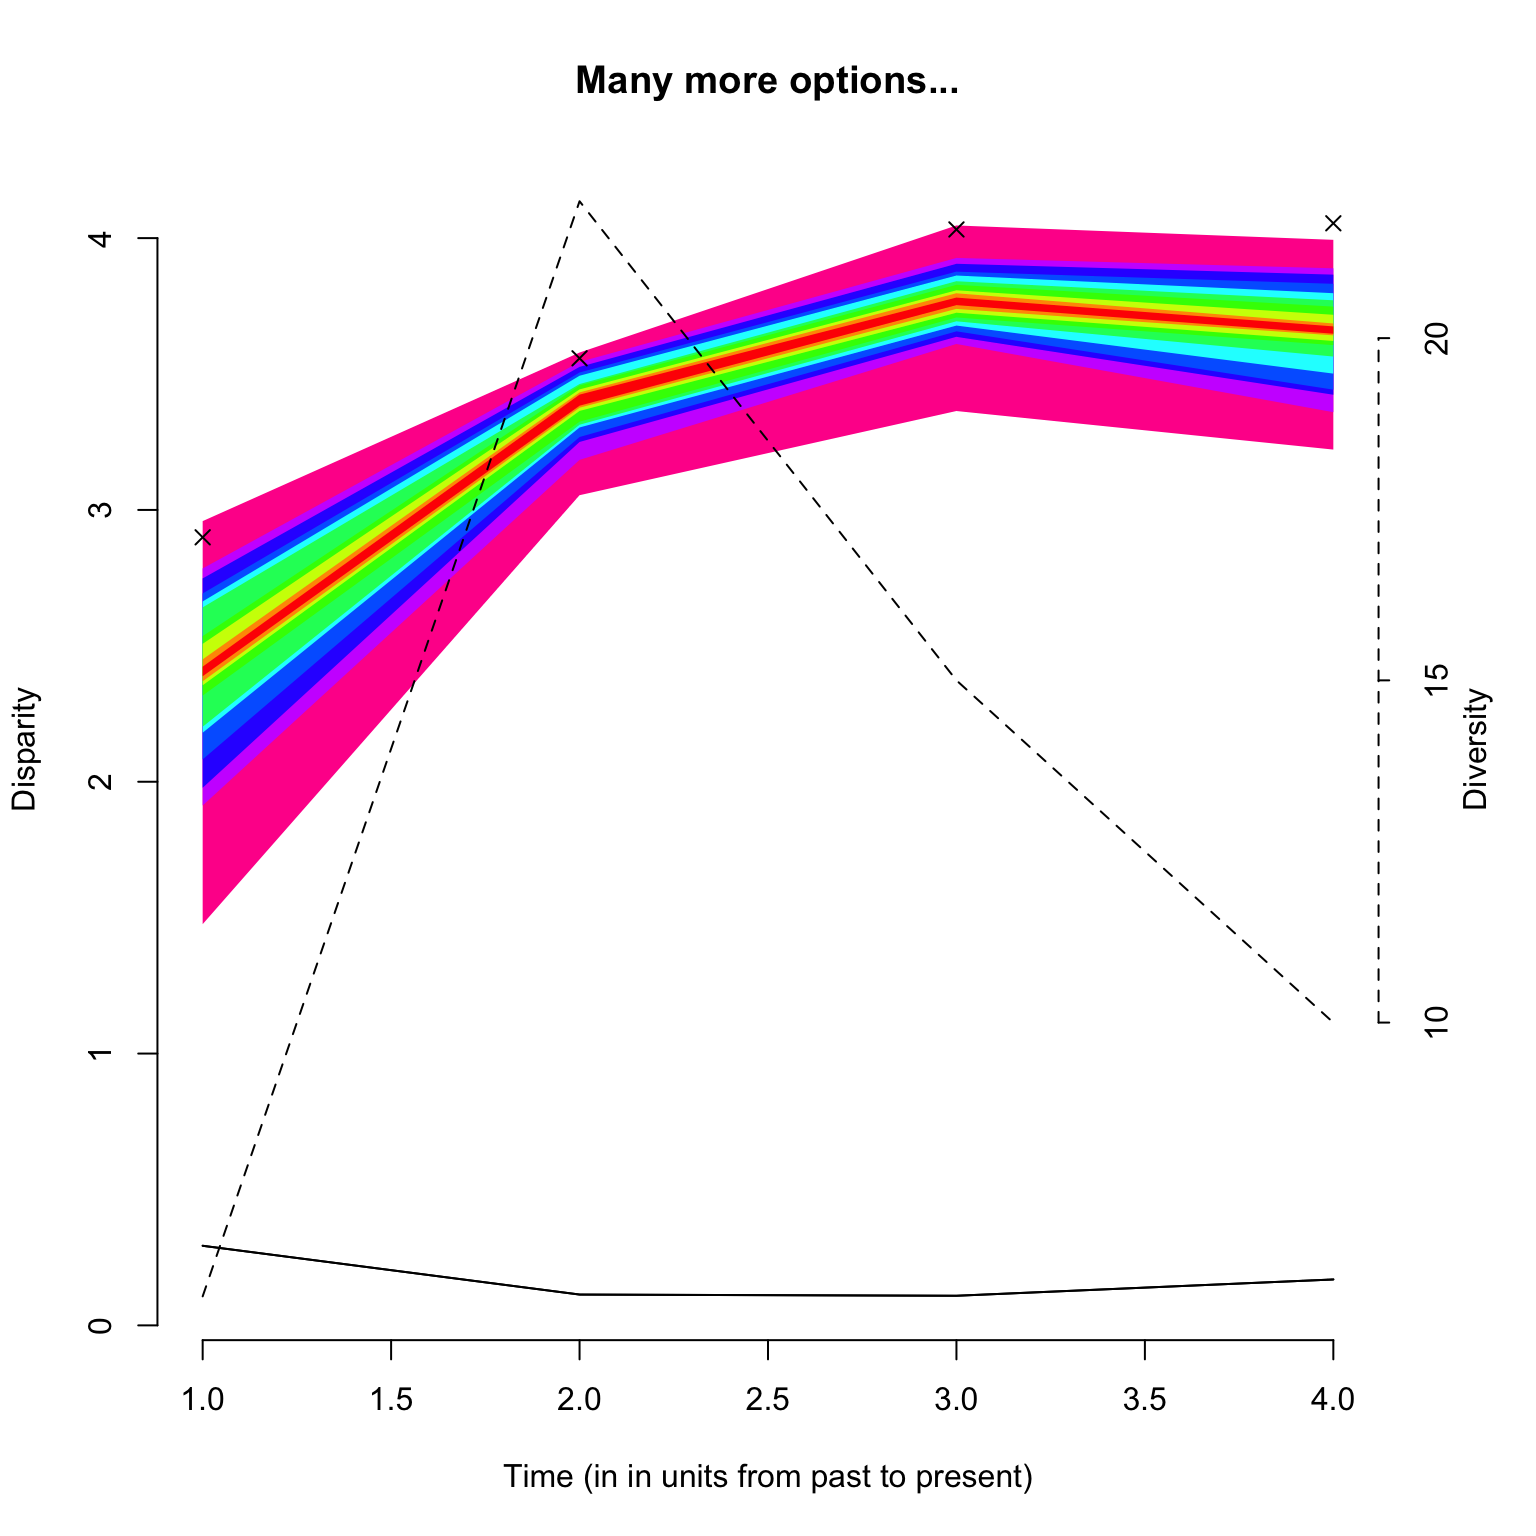
\includegraphics{dispRity_manual_files/figure-latex/unnamed-chunk-49-1.pdf}

\begin{Shaded}
\begin{Highlighting}[]
\NormalTok{## Resetting graphical parameters}
\KeywordTok{par}\NormalTok{(op)}
\end{Highlighting}
\end{Shaded}

\begin{quote}
Note that the argument \texttt{observed\ =\ TRUE} allows to plot the
disparity values calculated from the non-bootstrapped data as crosses on
the plot.
\end{quote}

For comparing results, it is also possible to add a plot to the existent
plot by using \texttt{add\ =\ TRUE}:

\begin{Shaded}
\begin{Highlighting}[]
\NormalTok{## Graphical options}
\NormalTok{op <-}\StringTok{ }\KeywordTok{par}\NormalTok{(}\DataTypeTok{bty =} \StringTok{"n"}\NormalTok{)}

\NormalTok{## Plotting the continuous disparity with a fixed y axis}
\KeywordTok{plot}\NormalTok{(disparity_time_slices, }\DataTypeTok{ylim =} \KeywordTok{c}\NormalTok{(}\DecValTok{1}\NormalTok{, }\DecValTok{4}\NormalTok{))}
\NormalTok{## Adding the discrete data}
\KeywordTok{plot}\NormalTok{(disparity_time_bins, }\DataTypeTok{type =} \StringTok{"line"}\NormalTok{, }\DataTypeTok{ylim =} \KeywordTok{c}\NormalTok{(}\DecValTok{1}\NormalTok{, }\DecValTok{4}\NormalTok{), }\DataTypeTok{xlab =} \StringTok{""}\NormalTok{, }\DataTypeTok{ylab =} \StringTok{""}\NormalTok{,}
    \DataTypeTok{add =} \OtherTok{TRUE}\NormalTok{)}
\end{Highlighting}
\end{Shaded}

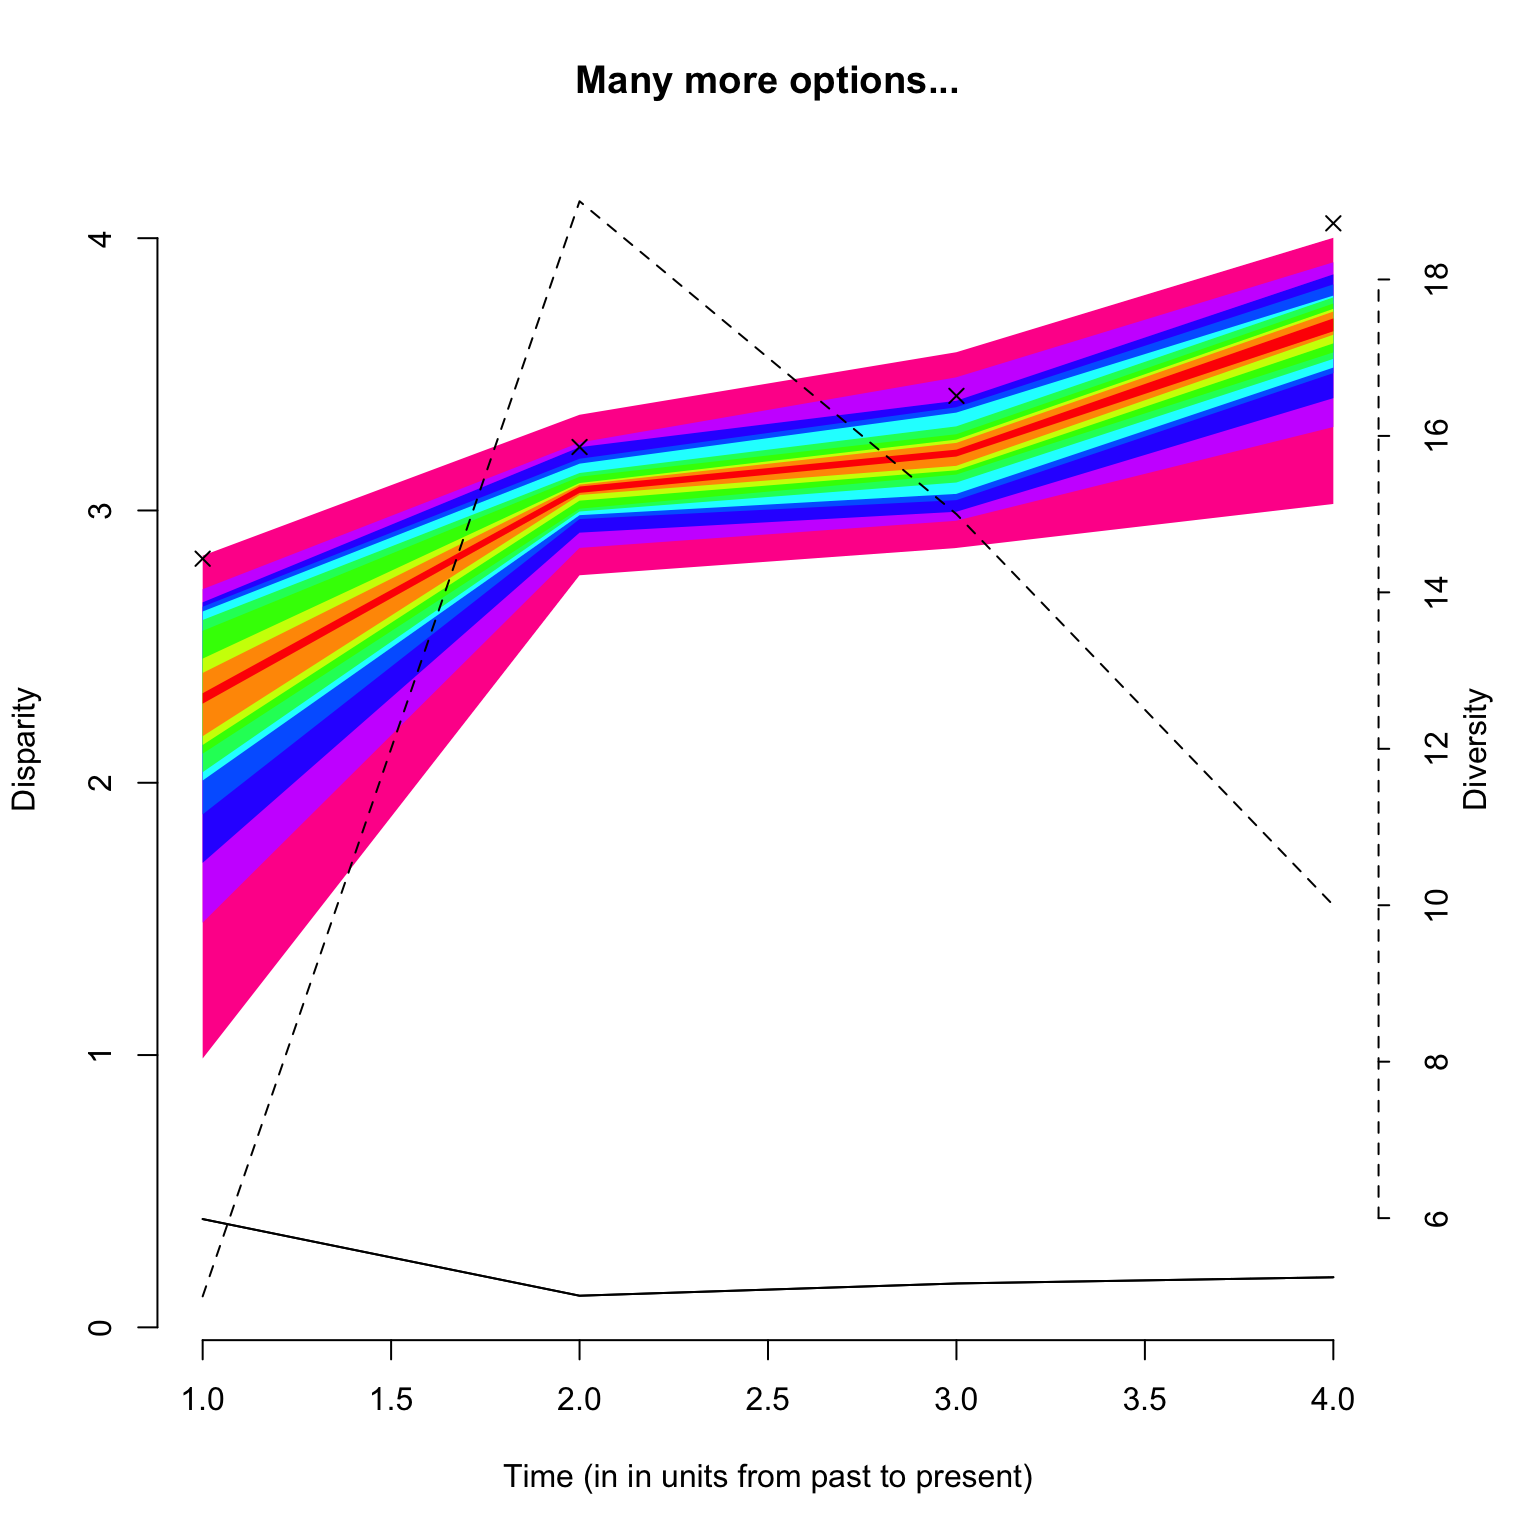
\includegraphics{dispRity_manual_files/figure-latex/unnamed-chunk-50-1.pdf}

\begin{Shaded}
\begin{Highlighting}[]
\NormalTok{## Resetting graphical parameters}
\KeywordTok{par}\NormalTok{(op)}
\end{Highlighting}
\end{Shaded}

Finally, if your data has been fully rarefied, it is also possible to
easily look at rarefaction curves by using the
\texttt{rarefaction\ =\ TRUE} argument:

\begin{Shaded}
\begin{Highlighting}[]
\NormalTok{## Graphical options}
\NormalTok{op <-}\StringTok{ }\KeywordTok{par}\NormalTok{(}\DataTypeTok{bty =} \StringTok{"n"}\NormalTok{)}

\NormalTok{## Plotting the rarefaction curves}
\KeywordTok{plot}\NormalTok{(disparity_crown_stem, }\DataTypeTok{rarefaction =} \OtherTok{TRUE}\NormalTok{)}
\end{Highlighting}
\end{Shaded}

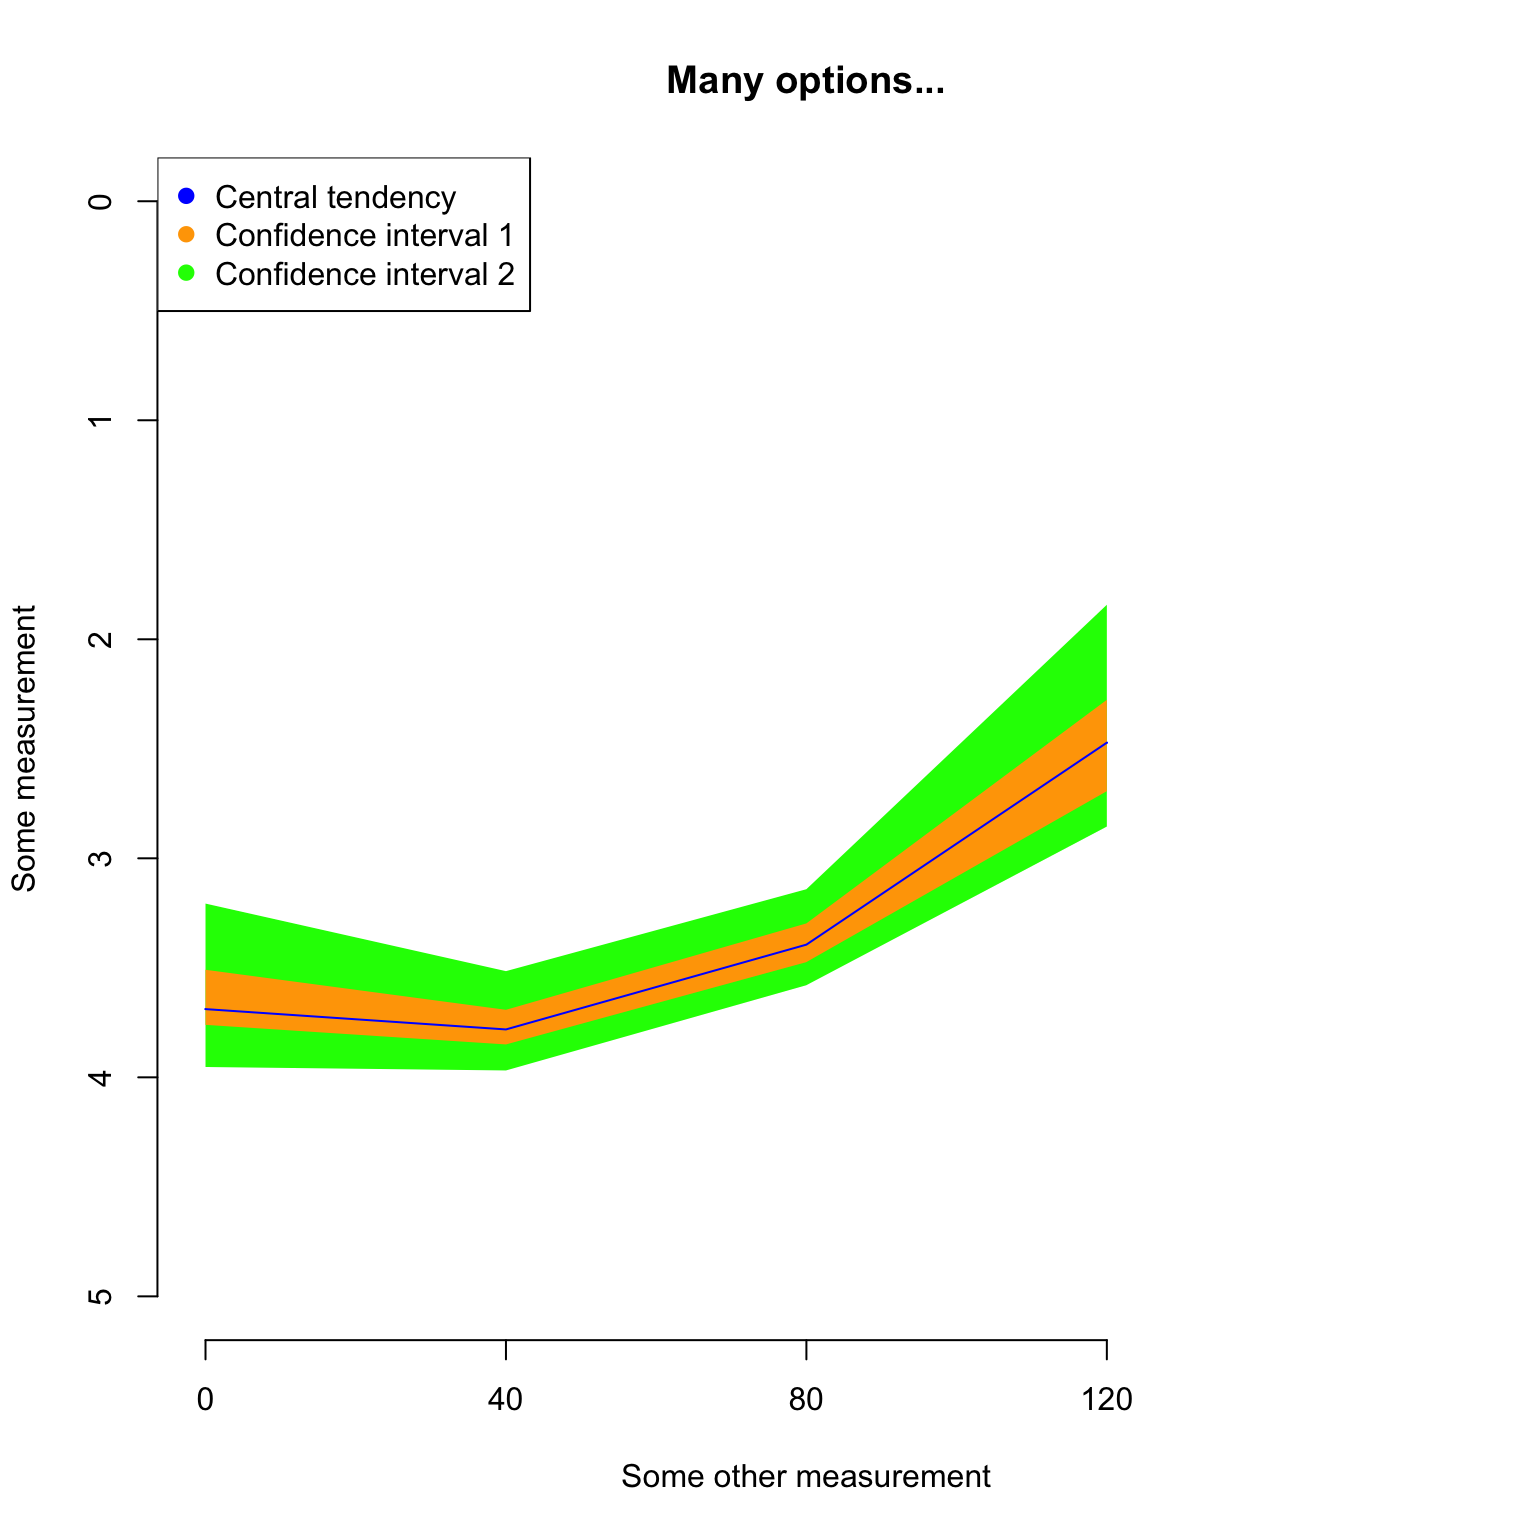
\includegraphics{dispRity_manual_files/figure-latex/unnamed-chunk-51-1.pdf}

\begin{Shaded}
\begin{Highlighting}[]
\NormalTok{## Resetting graphical parameters}
\KeywordTok{par}\NormalTok{(op)}
\end{Highlighting}
\end{Shaded}

\section{Testing disparity
hypotheses}\label{testing-disparity-hypotheses}

The \texttt{dispRity} package allows users to apply statistical tests to
the calculated disparity to test various hypotheses. The function
\texttt{test.dispRity} works in a similar way to the \texttt{dispRity}
function: it takes a \texttt{dispRity} object, a \texttt{test} and a
\texttt{comparisons} argument.

The \texttt{comparisons} argument indicates the way the test should be
applied to the data:

\begin{itemize}
\tightlist
\item
  \texttt{pairwise} (default): to compare each subsample in a pairwise
  manner
\item
  \texttt{referential}: to compare each subsample to the first subsample
\item
  \texttt{sequential}: to compare each subsample to the following
  subsample
\item
  \texttt{all}: to compare all the subsamples together (like in analysis
  of variance)
\end{itemize}

It is also possible to input a list of pairs of \texttt{numeric} values
or \texttt{characters} matching the subsample names to create
personalised tests. Some other tests implemented in \texttt{dispRity}
such as the \texttt{dispRity::null.test} have a specific way they are
applied to the data and therefore ignore the \texttt{comparisons}
argument.

The \texttt{test} argument can be any statistical or non-statistical
test to apply to the disparity object. It can be a common statistical
test function (e.g. \texttt{stats::t.test}), a function implemented in
\texttt{dispRity} (e.g.~see \texttt{?null.test}) or any function defined
by the user.

This function also allows users to correct for Type I error inflation
(false positives) when using multiple comparisons via the
\texttt{correction} argument. This argument can be empty (no correction
applied) or can contain one of the corrections from the
\texttt{stats::p.adjust} function (see \texttt{?p.adjust}).

Note that the \texttt{test.dispRity} algorithm deals with some classical
test outputs (\texttt{h.test}, \texttt{lm} and \texttt{numeric} vector)
and summarises the test output. It is, however, possible to get the full
detailed output by using the options \texttt{details\ =\ TRUE}.

Here we are using the variables generated in the
\protect\hyperlink{summarising-dispRity-data-plots}{section above}:

\begin{Shaded}
\begin{Highlighting}[]
\NormalTok{## T-test to test for a difference in disparity between crown and stem mammals}
\KeywordTok{test.dispRity}\NormalTok{(disparity_crown_stem, }\DataTypeTok{test =}\NormalTok{ t.test)}
\end{Highlighting}
\end{Shaded}

\begin{verbatim}
## Warning in test.dispRity(disparity_crown_stem, test = t.test): Multiple p-values will be calculated without adjustment!
## This will inflate Type I error!
\end{verbatim}

\begin{verbatim}
## [[1]]
##              statistic
## crown : stem  57.80615
## 
## [[2]]
##              parameter
## crown : stem  168.7267
## 
## [[3]]
##                    p.value
## crown : stem 3.927248e-113
\end{verbatim}

\begin{Shaded}
\begin{Highlighting}[]
\NormalTok{## Performing the same test but with the detailed t.test output}
\KeywordTok{test.dispRity}\NormalTok{(disparity_crown_stem, }\DataTypeTok{test =}\NormalTok{ t.test, }\DataTypeTok{details =} \OtherTok{TRUE}\NormalTok{)}
\end{Highlighting}
\end{Shaded}

\begin{verbatim}
## Warning in test.dispRity(disparity_crown_stem, test = t.test, details = TRUE): Multiple p-values will be calculated without adjustment!
## This will inflate Type I error!
\end{verbatim}

\begin{verbatim}
## $`crown : stem`
## $`crown : stem`[[1]]
## 
##  Welch Two Sample t-test
## 
## data:  dots[[1L]][[1L]] and dots[[2L]][[1L]]
## t = 57.806, df = 168.73, p-value < 2.2e-16
## alternative hypothesis: true difference in means is not equal to 0
## 95 percent confidence interval:
##  0.2843010 0.3044058
## sample estimates:
## mean of x mean of y 
##  1.926709  1.632356
\end{verbatim}

\begin{Shaded}
\begin{Highlighting}[]
\NormalTok{## Wilcoxon test applied to time sliced disparity with sequential comparisons,}
\NormalTok{## with Bonferroni correction}
\KeywordTok{test.dispRity}\NormalTok{(disparity_time_slices, }\DataTypeTok{test =}\NormalTok{ wilcox.test,}
              \DataTypeTok{comparisons =} \StringTok{"sequential"}\NormalTok{, }\DataTypeTok{correction =} \StringTok{"bonferroni"}\NormalTok{)}
\end{Highlighting}
\end{Shaded}

\begin{verbatim}
## [[1]]
##          statistic
## 120 : 80        30
## 80 : 40       2683
## 40 : 0         333
## 
## [[2]]
##               p.value
## 120 : 80 1.878222e-33
## 80 : 40  4.538271e-08
## 40 : 0   1.224822e-29
\end{verbatim}

\begin{Shaded}
\begin{Highlighting}[]
\NormalTok{## Measuring the overlap between distributions in the time bins (using the}
\NormalTok{## implemented Bhattacharyya Coefficient function - see ?bhatt.coeff)}
\KeywordTok{test.dispRity}\NormalTok{(disparity_time_bins, }\DataTypeTok{test =}\NormalTok{ bhatt.coeff)}
\end{Highlighting}
\end{Shaded}

\begin{verbatim}
## Warning in test.dispRity(disparity_time_bins, test = bhatt.coeff): Multiple p-values will be calculated without adjustment!
## This will inflate Type I error!
\end{verbatim}

\begin{verbatim}
##                    bhatt.coeff
## 120 - 80 : 80 - 40   0.0000000
## 120 - 80 : 40 - 0    0.0000000
## 80 - 40 : 40 - 0     0.3961442
\end{verbatim}

It is also possible to apply some more \emph{complex} tests that have
their own output classes (like \texttt{stats::lm}).

The results can then be analysed as usual using the associated
\texttt{summary} S3 method:

\begin{Shaded}
\begin{Highlighting}[]
\NormalTok{## Performing and linear model applied to the same data}
\NormalTok{(slice_lm <-}\StringTok{ }\KeywordTok{test.dispRity}\NormalTok{(disparity_time_slices, }\DataTypeTok{test =}\NormalTok{ lm,}
                            \DataTypeTok{comparisons =} \StringTok{"all"}\NormalTok{))}
\end{Highlighting}
\end{Shaded}

\begin{verbatim}
## Warning in test.dispRity(disparity_time_slices, test = lm, comparisons = "all"): Multiple p-values will be calculated without adjustment!
## This will inflate Type I error!
\end{verbatim}

\begin{verbatim}
## 
## Call:
## test(formula = data ~ subsamples, data = data)
## 
## Coefficients:
##   (Intercept)  subsamples120   subsamples40   subsamples80  
##        3.6607        -1.4176        -0.4820        -0.6138
\end{verbatim}

\begin{Shaded}
\begin{Highlighting}[]
\NormalTok{## The output is a regular `lm` output}
\KeywordTok{class}\NormalTok{(slice_lm)}
\end{Highlighting}
\end{Shaded}

\begin{verbatim}
## [1] "lm"
\end{verbatim}

\begin{Shaded}
\begin{Highlighting}[]
\NormalTok{## This output can be summarised using summary}
\KeywordTok{summary}\NormalTok{(slice_lm)}
\end{Highlighting}
\end{Shaded}

\begin{verbatim}
## 
## Call:
## test(formula = data ~ subsamples, data = data)
## 
## Residuals:
##      Min       1Q   Median       3Q      Max 
## -1.32553 -0.12305  0.02008  0.14801  0.59102 
## 
## Coefficients:
##               Estimate Std. Error t value Pr(>|t|)    
## (Intercept)    3.66072    0.02497  146.60   <2e-16 ***
## subsamples120 -1.41761    0.03531  -40.14   <2e-16 ***
## subsamples40  -0.48195    0.03531  -13.65   <2e-16 ***
## subsamples80  -0.61382    0.03531  -17.38   <2e-16 ***
## ---
## Signif. codes:  0 '***' 0.001 '**' 0.01 '*' 0.05 '.' 0.1 ' ' 1
## 
## Residual standard error: 0.2497 on 396 degrees of freedom
## Multiple R-squared:  0.808,  Adjusted R-squared:  0.8066 
## F-statistic: 555.6 on 3 and 396 DF,  p-value: < 2.2e-16
\end{verbatim}

Of course, due to the modular design of the package, tests can always be
made by the user (the same way disparity metrics can be user made). The
only condition is that the test can be applied to at least two
distributions. In practice, the \texttt{test.dispRity} function will
pass the calculated disparity data (distributions) to the provided
function in either pairs of distributions (if the \texttt{comparisons}
argument is set to \texttt{pairwise}, \texttt{referential} or
\texttt{sequential}) or a table containing all the distributions
(\texttt{comparisons\ =\ all}; this should be in the same format as data
passed to \texttt{lm} for example).

\hypertarget{disparity-as-a-distribution}{\section{Disparity as a
distribution}\label{disparity-as-a-distribution}}

Disparity is often regarded as a summary value of the position of the
all elements in the ordinated space. For example, the sum of variances,
the product of ranges or the median distance between the elements and
their centroid will summarise disparity as a single value. This value
can be pseudo-replicated (bootstrapped) to obtain a distribution of the
summary metric with estimated error. However, another way to perform
disparity analysis is to use the \emph{whole distribution} rather than
just a summary metric (e.g.~the variances or the ranges).

This is possible in the \texttt{dispRity} package by calculating
disparity as a dimension-level 2 metric only! Let's have a look using
our \protect\hyperlink{summarising-dispRity-data-plots}{previous
example} of bootstrapped time slices but by measuring the distances
between each taxon and their centroid as disparity.

\begin{Shaded}
\begin{Highlighting}[]
\NormalTok{## Measuring disparity as a whole distribution}
\NormalTok{disparity_centroids <-}\StringTok{ }\KeywordTok{dispRity}\NormalTok{(boot_time_slices, }\DataTypeTok{metric =}\NormalTok{ centroids)}
\end{Highlighting}
\end{Shaded}

The resulting disparity object is of dimension-level 2, so it can easily
be transformed into a dimension-level 1 object by, for example,
measuring the median distance of all these distributions:

\begin{Shaded}
\begin{Highlighting}[]
\NormalTok{## Measuring median disparity in each time slice}
\NormalTok{disparity_centroids_median <-}\StringTok{ }\KeywordTok{dispRity}\NormalTok{(disparity_centroids, }\DataTypeTok{metric =}\NormalTok{ median)}
\end{Highlighting}
\end{Shaded}

And we can now compare the differences between these methods:

\begin{Shaded}
\begin{Highlighting}[]
\NormalTok{## Summarising both disparity measurements:}
\NormalTok{## The distributions:}
\KeywordTok{summary}\NormalTok{(disparity_centroids)}
\end{Highlighting}
\end{Shaded}

\begin{verbatim}
##   subsamples  n obs.median bs.median  2.5%   25%   75% 97.5%
## 1        120  5      1.508     1.313 0.690 1.109 1.554 1.843
## 2         80 19      1.790     1.692 1.373 1.589 1.813 1.942
## 3         40 15      1.719     1.700 1.321 1.564 1.860 2.053
## 4          0 10      1.910     1.815 1.390 1.705 1.961 2.096
\end{verbatim}

\begin{Shaded}
\begin{Highlighting}[]
\NormalTok{## The summary of the distributions (as median)}
\KeywordTok{summary}\NormalTok{(disparity_centroids_median)}
\end{Highlighting}
\end{Shaded}

\begin{verbatim}
##   subsamples  n   obs bs.median  2.5%   25%   75% 97.5%
## 1        120  5 1.508     1.354 0.690 0.883 1.475 1.508
## 2         80 19 1.790     1.690 1.577 1.645 1.734 1.782
## 3         40 15 1.719     1.696 1.559 1.648 1.755 1.824
## 4          0 10 1.910     1.818 1.579 1.786 1.860 1.921
\end{verbatim}

We can see that the summary message for the distribution is slightly
different than before. Here \texttt{summary} also displays the observed
central tendency (i.e.~the central tendency of the measured
distributions). Note that, as expected, this central tendency is the
same in both metrics!

Another, maybe more intuitive way, to compare both approaches for
measuring disparity is to plot the distributions:

\begin{Shaded}
\begin{Highlighting}[]
\NormalTok{## Graphical parameters}
\NormalTok{op <-}\StringTok{ }\KeywordTok{par}\NormalTok{(}\DataTypeTok{bty =} \StringTok{"n"}\NormalTok{, }\DataTypeTok{mfrow =} \KeywordTok{c}\NormalTok{(}\DecValTok{1}\NormalTok{, }\DecValTok{2}\NormalTok{))}

\NormalTok{## Plotting both disparity measurements}
\KeywordTok{plot}\NormalTok{(disparity_centroids, }\DataTypeTok{ylab =} \StringTok{"Distribution of all the distances"}\NormalTok{)}
\KeywordTok{plot}\NormalTok{(disparity_centroids_median,}
     \DataTypeTok{ylab =} \StringTok{"Distribution of the medians of all the distances"}\NormalTok{)}
\end{Highlighting}
\end{Shaded}

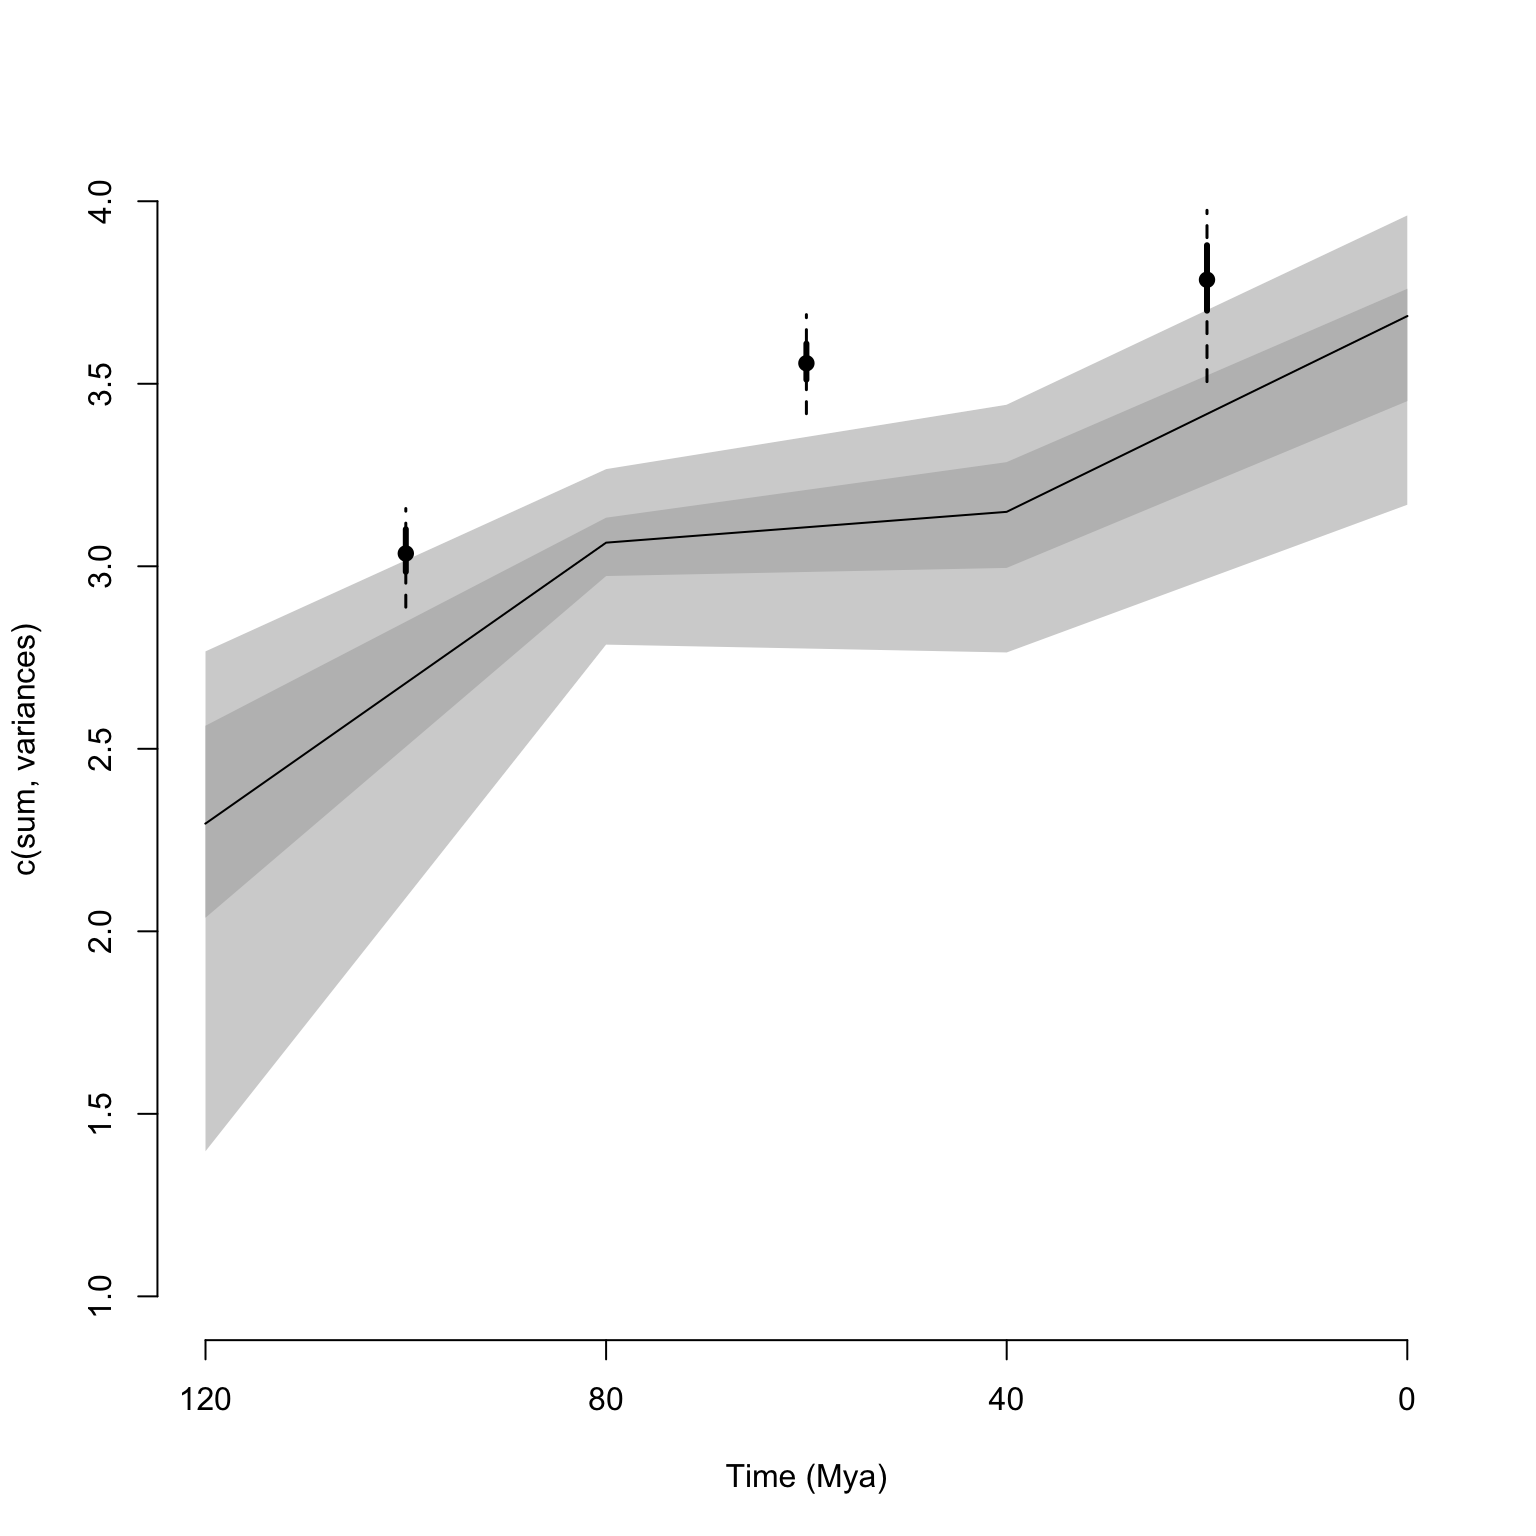
\includegraphics{dispRity_manual_files/figure-latex/unnamed-chunk-57-1.pdf}

\begin{Shaded}
\begin{Highlighting}[]
\KeywordTok{par}\NormalTok{(op)}
\end{Highlighting}
\end{Shaded}

We can then test for differences in the resulting distributions using
\texttt{test.dispRity} and the \texttt{bhatt.coeff} test as described
above.

\begin{Shaded}
\begin{Highlighting}[]
\NormalTok{## Probability of overlap in the distribution of medians}
\KeywordTok{test.dispRity}\NormalTok{(disparity_centroids_median, }\DataTypeTok{test =}\NormalTok{ bhatt.coeff)}
\end{Highlighting}
\end{Shaded}

\begin{verbatim}
## Warning in test.dispRity(disparity_centroids_median, test = bhatt.coeff): Multiple p-values will be calculated without adjustment!
## This will inflate Type I error!
\end{verbatim}

\begin{verbatim}
##          bhatt.coeff
## 120 : 80  0.02645751
## 120 : 40  0.07348469
## 120 : 0   0.03162278
## 80 : 40   0.91611371
## 80 : 0    0.46010984
## 40 : 0    0.62247224
\end{verbatim}

In this case, we are looking at the probability of overlap of the
distribution of median distances from centroids among each pair of time
slices. In other words, we are measuring whether the medians from each
bootstrap pseudo-replicate for each time slice overlap. But of course,
we might be interested in the actual distribution of the distances from
the centroid rather than simply their central tendencies. This can be
problematic depending on the research question asked since we are
effectively comparing non-independent medians distributions (because of
the pseudo-replication).

One solution, therefore, is to look at the full distribution:

\begin{Shaded}
\begin{Highlighting}[]
\NormalTok{## Probability of overlap for the full distributions}
\KeywordTok{test.dispRity}\NormalTok{(disparity_centroids, }\DataTypeTok{test =}\NormalTok{ bhatt.coeff)}
\end{Highlighting}
\end{Shaded}

\begin{verbatim}
## Warning in test.dispRity(disparity_centroids, test = bhatt.coeff): Multiple p-values will be calculated without adjustment!
## This will inflate Type I error!
\end{verbatim}

\begin{verbatim}
##          bhatt.coeff
## 120 : 80   0.6565552
## 120 : 40   0.6767954
## 120 : 0    0.5410092
## 80 : 40    0.9355145
## 80 : 0     0.8571521
## 40 : 0     0.9303364
\end{verbatim}

These results show the actual overlap among all the measured distances
from centroids concatenated across all the bootstraps. For example, when
comparing the slices 120 and 80, we are effectively comparing the 5
\(\times\) 100 distances (the distances of the five elements in slice
120 bootstrapped 100 times) to the 19 \(\times\) 100 distances from
slice 80. However, this can also be problematic for some specific tests
since the \emph{n} \(\times\) 100 distances are also pseudo-replicates
and thus are still not independent.

A second solution is to compare the distributions to each other
\emph{for each replicate}:

\begin{Shaded}
\begin{Highlighting}[]
\NormalTok{## Boostrapped probability of overlap for the full distributions}
\KeywordTok{test.dispRity}\NormalTok{(disparity_centroids, }\DataTypeTok{test =}\NormalTok{ bhatt.coeff, }\DataTypeTok{concatenate =} \OtherTok{FALSE}\NormalTok{)}
\end{Highlighting}
\end{Shaded}

\begin{verbatim}
## Warning in test.dispRity(disparity_centroids, test = bhatt.coeff, concatenate = FALSE): Multiple p-values will be calculated without adjustment!
## This will inflate Type I error!
\end{verbatim}

\begin{verbatim}
##          bhatt.coeff       2.5%       25%       75%     97.5%
## 120 : 80   0.2818787 0.00000000 0.1450953 0.4304156 0.6375038
## 120 : 40   0.3195364 0.00000000 0.2000000 0.4238587 0.7079195
## 120 : 0    0.2427199 0.00000000 0.1500000 0.3464102 0.5464102
## 80 : 40    0.6168602 0.34464773 0.5178144 0.7152871 0.8620129
## 80 : 0     0.4666682 0.04873397 0.3547815 0.6142885 0.7343247
## 40 : 0     0.5410387 0.19542869 0.4302200 0.6531298 0.8145697
\end{verbatim}

These results show the median overlap among pairs of distributions in
the first column (\texttt{bhatt.coeff}) and then the distribution of
these overlaps among each pair of bootstraps. In other words, when two
distributions are compared, they are now compared for each bootstrap
pseudo-replicate, thus effectively creating a distribution of
probabilities of overlap. For example, when comparing the slices 120 and
80, we have a mean probability of overlap of 0.28 and a probability
between 0.18 and 0.43 in 50\% of the pseudo-replicates. Note that the
quantiles and central tendencies can be modified via the
\texttt{conc.quantiles} option.

\chapter{Making stuff up!}\label{making-stuff-up}

The \texttt{dispRity} package also offers some advanced data simulation
features to allow to test hypothesis, explore ordinate-spaces or metrics
properties or simply playing around with data! All the following
functions are based on the same modular architecture of the package and
therefore can be used with most of the functions of the package.

\section{Simulating discrete morphological
data}\label{simulating-discrete-morphological-data}

The function \texttt{sim.morpho} allows to simulate discrete
morphological data matrices (sometimes referred to as ``cladistic''
matrices). It allows to evolve multiple discrete characters on a given
phylogenetic trees, given different models, rates, and states. It even
allows to include proper inapplicable data to make datasets as messy as
in real life!

In brief, the function \texttt{sim.morpho} takes a phylogenetic tree,
the number of required characters, the evolutionary model, and a
function from which to draw the rates. The package also contains a
function for quickly checking the matrix's phylogenetic signal (as
defined in systematics not phylogenetic comparative methods) using
parsimony. The methods are described in details below

\begin{Shaded}
\begin{Highlighting}[]
\KeywordTok{set.seed}\NormalTok{(}\DecValTok{3}\NormalTok{)}
\NormalTok{## Simulating a starting tree with 15 taxa as a random coalescent tree}
\NormalTok{my_tree <-}\StringTok{ }\KeywordTok{rcoal}\NormalTok{(}\DecValTok{15}\NormalTok{)}

\NormalTok{## Generating a matrix with 100 characters (85% binary and 15% three state) and}
\NormalTok{## an equal rates model with a gamma rate distribution (0.5, 1) with no }
\NormalTok{## invariant characters.}
\NormalTok{my_matrix <-}\StringTok{ }\KeywordTok{sim.morpho}\NormalTok{(}\DataTypeTok{tree =}\NormalTok{ my_tree, }\DataTypeTok{characters =} \DecValTok{100}\NormalTok{, }\DataTypeTok{states =} \KeywordTok{c}\NormalTok{(}\FloatTok{0.85}\NormalTok{,}
    \FloatTok{0.15}\NormalTok{), }\DataTypeTok{rates =} \KeywordTok{c}\NormalTok{(rgamma, }\FloatTok{0.5}\NormalTok{, }\DecValTok{1}\NormalTok{), }\DataTypeTok{invariant =} \OtherTok{FALSE}\NormalTok{)}

\NormalTok{## The first few lines of the matrix}
\NormalTok{my_matrix[}\DecValTok{1}\OperatorTok{:}\DecValTok{5}\NormalTok{, }\DecValTok{1}\OperatorTok{:}\DecValTok{10}\NormalTok{]}
\end{Highlighting}
\end{Shaded}

\begin{verbatim}
##     [,1] [,2] [,3] [,4] [,5] [,6] [,7] [,8] [,9] [,10]
## t15 "1"  "1"  "0"  "1"  "1"  "2"  "1"  "1"  "0"  "0"  
## t12 "1"  "1"  "0"  "1"  "1"  "2"  "1"  "1"  "0"  "0"  
## t14 "1"  "1"  "0"  "1"  "1"  "2"  "1"  "1"  "0"  "0"  
## t6  "1"  "1"  "0"  "1"  "1"  "2"  "1"  "1"  "0"  "0"  
## t3  "0"  "0"  "1"  "0"  "1"  "0"  "0"  "2"  "1"  "0"
\end{verbatim}

\begin{Shaded}
\begin{Highlighting}[]
\NormalTok{## Checking the matrix properties with a quick Maximum Parsimony tree search}
\KeywordTok{check.morpho}\NormalTok{(my_matrix, my_tree)}
\end{Highlighting}
\end{Shaded}

\begin{verbatim}
##                                     
## Maximum parsimony        139.0000000
## Consistency index          0.7625899
## Retention index            0.8881356
## Robinson-Foulds distance   0.0000000
\end{verbatim}

Note that this example produces a tree with a great consistency index
and an identical topology to the random coalescent tree! Nearly too good
to be true\ldots{}

\subsection{A more detailed
description}\label{a-more-detailed-description}

The protocol implemented here to generate discrete morphological
matrices is based on the ones developed in
{[}\citet{GuillermeCooper};\citet{OReilly2016};\citet{puttick2017uncertain};OReilly2017{]}.

\begin{itemize}
\tightlist
\item
  The first \texttt{tree} argument will be the tree on which to
  ``evolve'' the characters and therefore requires branch length. You
  can generate quick and easy random Yule trees using
  \texttt{ape::rtree(number\_of\_taxa)} but I would advise to use more
  realistic trees for more realistic simulations based on more realistic
  models (really realistic then) using the function \texttt{tree.bd}
  from the
  \href{http://www.zoology.ubc.ca/prog/diversitree/}{\texttt{diversitree}}
  package \citep{fitzjohndiversitree2012}.
\item
  The second argument, \texttt{character} is the number of characters.
  Pretty straight forward.
\item
  The third, \texttt{states} is the proportion of characters states
  above two (yes, the minimum number of states is two). This argument
  intakes the proportion of \emph{n}-states characters, for example
  \texttt{states\ =\ c(0.5,0.3,0.2)} will generate 50\% of binary-state
  characters, 30\% of three-state characters and 20\% of four-state
  characters. There is no limit in the number of state characters
  proportion as long as the total makes up 100\%.
\item
  The forth, \texttt{model} is the evolutionary model for generating the
  character(s). More about this below.
\item
  The fifth and sixth, \texttt{rates} and \texttt{substitution} are the
  model parameters described below as well.
\item
  Finally, the two logical arguments, are self explanatory:
  \texttt{invariant} whether to allow invariant characters
  (i.e.~characters that don't change) and \texttt{verbose} whether to
  print the simulation progress on your console.
\end{itemize}

\subsubsection{Available evolutionary
models}\label{available-evolutionary-models}

There are currently three evolutionary models implemented in
\texttt{sim.morpho} but more will come in the future. Note also that
they allow fine tuning parameters making them pretty plastic!

\begin{itemize}
\tightlist
\item
  \texttt{"ER"}: this model allows any number of character states and is
  based on the Mk model \citep{lewisa2001}. It assumes a unique overall
  evolutionary rate equal substitution rate between character states.
  This model is based on the \texttt{ape::rTraitDisc} function.
\item
  \texttt{"HKY"}: this is binary state character model based on the
  molecular HKY model \citep{HKY85}. It uses the four molecular states
  (A,C,G,T) with a unique overall evolutionary rate and a biased
  substitution rate towards transitions (A \textless{}-\textgreater{} G
  or C \textless{}-\textgreater{} T) against transvertions (A
  \textless{}-\textgreater{} C and G \textless{}-\textgreater{} T).
  After evolving the nucleotide, this model transforms them into binary
  states by converting the purines (A and G) into state 0 and the
  pyrimidines (C and T) into state 1. This method is based on the
  \texttt{phyclust::seq.gen.HKY} function and was first proposed by
  \citet{OReilly2016}.
\item
  \texttt{"MIXED"}: this model uses a random (uniform) mix between both
  the \texttt{"ER"} and the \texttt{"HKY"} models.
\end{itemize}

The models can take the following parameters: (1) \texttt{rates} is the
evolutionary rate (i.e.~the rate of changes along a branch: the
evolutionary speed) and (2) \texttt{substitution} is the frequency of
changes between one state or another. For example if a character can
have high probability of changing (the \emph{evolutionary} rate) with,
each time a change occurs a probability of changing from state \emph{X}
to state \emph{Y} (the \emph{substitution} rate). Note that in the
\texttt{"ER"} model, the substitution rate is ignore because\ldots{} by
definition this (substitution) rate is equal!

The parameters arguments \texttt{rates} and \texttt{substitution} takes
a distributions from which to draw the parameters values for each
character. For example, if you want an \texttt{"HKY"} model with an
evolutionary rate (i.e.~speed) drawn from a uniform distribution bounded
between 0.001 and 0.005, you can define it as
\texttt{rates\ =\ c(runif,\ min\ =\ 0.001,\ max\ =\ 0.005)},
\texttt{runif} being the function for random draws from a uniform
distribution and \texttt{max} and \texttt{min} being the distribution
parameters. These distributions should always be passed in the format
\texttt{c(random\_distribution\_function,\ distribution\_parameters)}
with the names of the distribution parameters arguments.

\subsubsection{Checking the results}\label{checking-the-results}

An additional function, \texttt{check.morpho} runs a quick Maximum
Parsimony tree search using the \texttt{phangorn} parsimony algorithm.
It quickly calculates the parsimony score, the consistency and retention
indices and, if a tree is provided (e.g.~the tree used to generate the
matrix) it calculates the Robinson-Foulds distance between the most
parsimonious tree and the provided tree to determine how different they
are.

\subsubsection{Adding inapplicable
characters}\label{adding-inapplicable-characters}

Once a matrix is generated, it is possible to apply inapplicable
characters to it for increasing realism! Inapplicable characters are
commonly designated as \texttt{NA} or simply \texttt{-}. They differ
from missing characters \texttt{?} in their nature by being inapplicable
rather than unknown. For example, considering a binary character defined
as ``colour of the tail'' with the following states ``blue'' and
``red''; on a taxa with no tail, the character should be coded as
inapplicable (``\texttt{-}'') since the state of the character ``colour
of tail'' is \emph{known}: it's neither ``blue'' or ``red'', it's just
not there! It contrasts with coding it as missing (``\texttt{?}'' - also
called as ambiguous) where the state is \emph{unknown}, for example, the
taxon of interest is a fossil where the tail has no colour preserved or
is not present at all due to bad conservation!

This type of characters can be added to the simulated matrices using the
\texttt{apply.NA} function/ It takes, as arguments, the \texttt{matrix},
the source of inapplicability (\texttt{NAs} - more below), the
\texttt{tree} used to generate the matrix and the two same
\texttt{invariant} and \texttt{verbose} arguments as defined above. The
\texttt{NAs} argument allows two types of sources of inapplicability:

\begin{itemize}
\tightlist
\item
  \texttt{"character"} where the inapplicability is due to the character
  (e.g.~coding a character tail for species with no tail). In practice,
  the algorithm chooses a character \emph{X} as the underlying character
  (e.g. ``presence and absence of tail''), arbitrarily chooses one of
  the states as ``absent'' (e.g.~0 = absent) and changes in the next
  character \emph{Y} any state next to character \emph{X} state 0 into
  an inapplicable token (``\texttt{-}''). This simulates the
  inapplicability induced by coding the characters (i.e.~not always
  biological).
\item
  \texttt{"clade"} where the inapplicability is due to evolutionary
  history (e.g.~a clade loosing its tail). In practice, the algorithm
  chooses a random clade in the tree and a random character \emph{Z} and
  replaces the state of the taxa present in the clade by the
  inapplicable token (``\texttt{-}''). This simulates the
  inapplicability induced by evolutionary biology (e.g.~the lose of a
  feature in a clade).
\end{itemize}

To apply these sources of inapplicability, simply repeat the number of
inapplicable sources for the desired number of characters with
inapplicable data.

\begin{Shaded}
\begin{Highlighting}[]
\NormalTok{## Generating 5 "character" NAs and 10 "clade" NAs}
\NormalTok{my_matrix_NA <-}\StringTok{ }\KeywordTok{apply.NA}\NormalTok{(my_matrix, }\DataTypeTok{tree =}\NormalTok{ my_tree,}
                         \DataTypeTok{NAs =} \KeywordTok{c}\NormalTok{(}\KeywordTok{rep}\NormalTok{(}\StringTok{"character"}\NormalTok{, }\DecValTok{5}\NormalTok{), }\KeywordTok{rep}\NormalTok{(}\StringTok{"clade"}\NormalTok{, }\DecValTok{10}\NormalTok{)))}

\NormalTok{## The first few lines of the resulting matrix}
\NormalTok{my_matrix_NA[}\DecValTok{1}\OperatorTok{:}\DecValTok{10}\NormalTok{, }\DecValTok{90}\OperatorTok{:}\DecValTok{100}\NormalTok{]}
\end{Highlighting}
\end{Shaded}

\begin{verbatim}
##     [,1] [,2] [,3] [,4] [,5] [,6] [,7] [,8] [,9] [,10] [,11]
## t15 "0"  "1"  "0"  "1"  "0"  "0"  "0"  "1"  "0"  "1"   "0"  
## t12 "1"  "1"  "0"  "1"  "0"  "0"  "0"  "1"  "0"  "1"   "0"  
## t14 "0"  "0"  "0"  "1"  "0"  "0"  "0"  "1"  "0"  "1"   "0"  
## t6  "0"  "0"  "0"  "1"  "0"  "0"  "0"  "1"  "0"  "1"   "0"  
## t3  "0"  "0"  "1"  "0"  "-"  "0"  "0"  "0"  "-"  "0"   "1"  
## t2  "0"  "0"  "1"  "0"  "-"  "0"  "0"  "0"  "-"  "0"   "1"  
## t11 "0"  "0"  "1"  "0"  "-"  "0"  "0"  "0"  "-"  "0"   "1"  
## t7  "0"  "0"  "1"  "0"  "-"  "0"  "0"  "0"  "-"  "0"   "1"  
## t1  "0"  "0"  "0"  "0"  "-"  "0"  "0"  "0"  "-"  "2"   "1"  
## t5  "0"  "0"  "0"  "0"  "-"  "0"  "0"  "0"  "-"  "0"   "1"
\end{verbatim}

\subsection{Parameters for a realistic(ish)
matrix}\label{parameters-for-a-realisticish-matrix}

There are many parameters that can create a ``realistic'' matrix
(i.e.~not too different from the input tree with a consistency and
retention index close to what is seen in the literature) but because of
the randomness of the matrix generation not all parameters combination
end up creating ``good'' matrices. The following parameters however,
seem to generate fairly ``realist'' matrices with a starting coalescent
tree, equal rates model with 0.85 binary characters and 0.15 three state
characters, a gamma distribution with a shape parameter (\(\alpha\)) of
5 and no scaling (\(\beta\) = 1) with a rate of 100.

\begin{Shaded}
\begin{Highlighting}[]
\KeywordTok{set.seed}\NormalTok{(}\DecValTok{0}\NormalTok{)}
\NormalTok{## tree}
\NormalTok{my_tree <-}\StringTok{ }\KeywordTok{rcoal}\NormalTok{(}\DecValTok{15}\NormalTok{)}
\NormalTok{## matrix}
\NormalTok{morpho_mat <-}\StringTok{ }\KeywordTok{sim.morpho}\NormalTok{(my_tree, }\DataTypeTok{characters =} \DecValTok{100}\NormalTok{, }\DataTypeTok{model =} \StringTok{"ER"}\NormalTok{,}
    \DataTypeTok{rates =} \KeywordTok{c}\NormalTok{(rgamma, }\DataTypeTok{rate =} \DecValTok{100}\NormalTok{, }\DataTypeTok{shape =} \DecValTok{5}\NormalTok{), }\DataTypeTok{invariant =} \OtherTok{FALSE}\NormalTok{)}
\KeywordTok{check.morpho}\NormalTok{(morpho_mat, my_tree)}
\end{Highlighting}
\end{Shaded}

\begin{verbatim}
##                                     
## Maximum parsimony        104.0000000
## Consistency index          0.0000000
## Retention index            0.7886179
## Robinson-Foulds distance   0.0000000
\end{verbatim}

\section{Simulating multidimensional
spaces}\label{simulating-multidimensional-spaces}

Another way to simulate data is to directly simulate an ordinated space
with the \texttt{space.maker} function. This function allows users to
simulate multidimensional spaces with a certain number of properties.
For example, it is possible to design a multidimensional space with a
specific distribution on each axis, a correlation between the axes and a
specific cumulative variance per axis. This can be useful for creating
ordinated spaces for null hypothesis, for example if you're using the
function \texttt{null.test} \citep{diaz2016global}.

This function takes as arguments the number of elements (data points -
\texttt{elements} argument)~and dimensions (\texttt{dimensions}
argument) to create the space and the distribution functions to be used
for each axis. The distributions are passed through the
\texttt{distribution} argument as\ldots{} modular functions! You can
either pass a single distribution function for all the axes (for example
\texttt{distribution\ =\ runif} for all the axis being uniform) or a
specific distribution function for each specific axis (for example
\texttt{distribution\ =\ c(runif,\ rnorm,\ rgamma))} for the first axis
being uniform, the second normal and the third gamma). You can of course
use your very own functions or use the ones implemented in
\texttt{dispRity} for more complex ones (see below). Specific optional
arguments for each of these distributions can be passed as a list via
the \texttt{arguments} argument.

Furthermore, it is possible to add a correlation matrix to add a
correlation between the axis via the \texttt{cor.matrix} argument or
even a vector of proportion of variance to be bear by each axis via the
\texttt{scree} argument to simulate realistic ordinated spaces.

Here is a simple two dimensional example:

\begin{Shaded}
\begin{Highlighting}[]
\NormalTok{## Graphical options}
\NormalTok{op <-}\StringTok{ }\KeywordTok{par}\NormalTok{(}\DataTypeTok{bty =} \StringTok{"n"}\NormalTok{)}

\NormalTok{## A square space}
\NormalTok{square_space <-}\StringTok{ }\KeywordTok{space.maker}\NormalTok{(}\DecValTok{100}\NormalTok{, }\DecValTok{2}\NormalTok{, runif)}

\NormalTok{## The resulting 2D matrix}
\KeywordTok{head}\NormalTok{(square_space)}
\end{Highlighting}
\end{Shaded}

\begin{verbatim}
##           [,1]       [,2]
## [1,] 0.9548679 0.55645395
## [2,] 0.3721235 0.53218069
## [3,] 0.3229877 0.25041834
## [4,] 0.8404244 0.46840450
## [5,] 0.2839796 0.07466592
## [6,] 0.2627652 0.24523019
\end{verbatim}

\begin{Shaded}
\begin{Highlighting}[]
\NormalTok{## Visualising the space}
\KeywordTok{plot}\NormalTok{(square_space, }\DataTypeTok{pch =} \DecValTok{20}\NormalTok{, }\DataTypeTok{xlab =} \StringTok{""}\NormalTok{, }\DataTypeTok{ylab =} \StringTok{""}\NormalTok{, }\DataTypeTok{main =} \StringTok{"Uniform 2D space"}\NormalTok{)}
\end{Highlighting}
\end{Shaded}

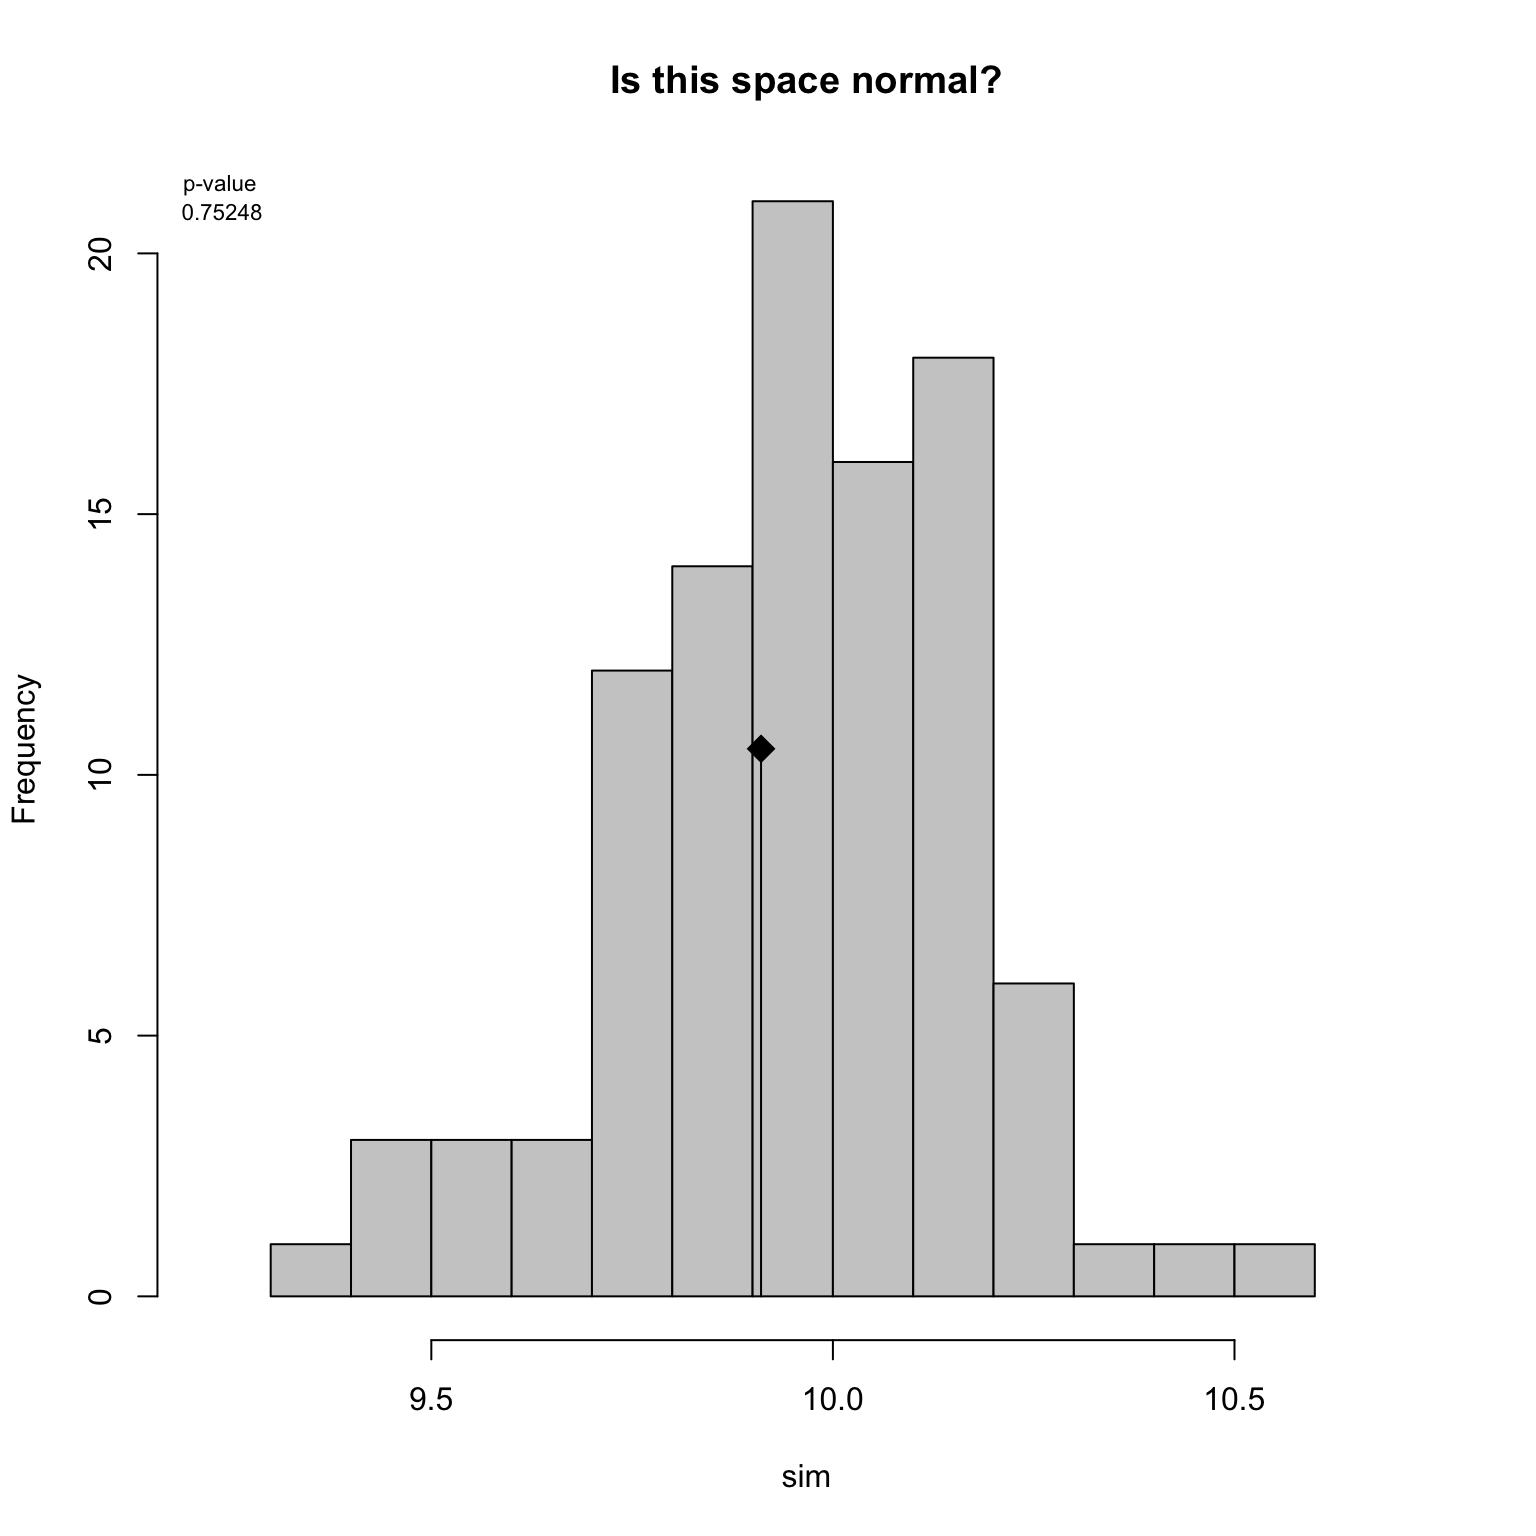
\includegraphics{dispRity_manual_files/figure-latex/unnamed-chunk-64-1.pdf}

Of course, more complex spaces can be created by changing the
distributions, their arguments or adding a correlation matrix or a
cumulative variance vector:

\begin{Shaded}
\begin{Highlighting}[]
\NormalTok{## A plane space: uniform with one dimensions equal to 0}
\NormalTok{plane_space <-}\StringTok{ }\KeywordTok{space.maker}\NormalTok{(}\DecValTok{2500}\NormalTok{, }\DecValTok{3}\NormalTok{, }\KeywordTok{c}\NormalTok{(runif, runif, runif),}
                           \DataTypeTok{arguments =} \KeywordTok{list}\NormalTok{(}\KeywordTok{list}\NormalTok{(}\DataTypeTok{min =} \DecValTok{0}\NormalTok{, }\DataTypeTok{max =} \DecValTok{0}\NormalTok{), }\OtherTok{NULL}\NormalTok{, }\OtherTok{NULL}\NormalTok{))}

\NormalTok{## Correlation matrix for a 3D space}
\NormalTok{(cor_matrix <-}\StringTok{ }\KeywordTok{matrix}\NormalTok{(}\KeywordTok{cbind}\NormalTok{(}\DecValTok{1}\NormalTok{, }\FloatTok{0.8}\NormalTok{, }\FloatTok{0.2}\NormalTok{, }\FloatTok{0.8}\NormalTok{, }\DecValTok{1}\NormalTok{, }\FloatTok{0.7}\NormalTok{, }\FloatTok{0.2}\NormalTok{, }\FloatTok{0.7}\NormalTok{, }\DecValTok{1}\NormalTok{), }\DataTypeTok{nrow =} \DecValTok{3}\NormalTok{))}
\end{Highlighting}
\end{Shaded}

\begin{verbatim}
##      [,1] [,2] [,3]
## [1,]  1.0  0.8  0.2
## [2,]  0.8  1.0  0.7
## [3,]  0.2  0.7  1.0
\end{verbatim}

\begin{Shaded}
\begin{Highlighting}[]
\NormalTok{## An ellipsoid space (normal space with correlation)}
\NormalTok{ellipse_space <-}\StringTok{ }\KeywordTok{space.maker}\NormalTok{(}\DecValTok{2500}\NormalTok{, }\DecValTok{3}\NormalTok{, rnorm, }\DataTypeTok{cor.matrix =}\NormalTok{ cor_matrix)}

\NormalTok{## A cylindrical space with decreasing axes variance}
\NormalTok{cylindrical_space <-}\StringTok{ }\KeywordTok{space.maker}\NormalTok{(}\DecValTok{2500}\NormalTok{, }\DecValTok{3}\NormalTok{, }\KeywordTok{c}\NormalTok{(rnorm, rnorm, runif),}
                                 \DataTypeTok{scree =} \KeywordTok{c}\NormalTok{(}\FloatTok{0.7}\NormalTok{, }\FloatTok{0.2}\NormalTok{, }\FloatTok{0.1}\NormalTok{))}
\end{Highlighting}
\end{Shaded}

\subsection{Personalised dimensions
distributions}\label{personalised-dimensions-distributions}

Following the modular architecture of the package, it is of course
possible to pass home made distribution functions to the
\texttt{distribution} argument. For example, the \texttt{random.circle}
function is a personalised one implemented in \texttt{dispRity}. This
function allows to create circles based on basic trigonometry allowing
to axis to covary to produce circle coordinates. By default, this
function generates two sets of coordinates with a \texttt{distribution}
argument and a minimum and maximum boundary (\texttt{inner} and
\texttt{outer} respectively) to create nice sharp edges to the circle.
The maximum boundary is equivalent to the radius of the circle (it
removes coordinates beyond the circle radius) and the minimum is
equivalent to the radius of a smaller circle with no data (it removes
coordinates below this inner circle radius).

\begin{Shaded}
\begin{Highlighting}[]
\NormalTok{## Graphical options}
\NormalTok{op <-}\StringTok{ }\KeywordTok{par}\NormalTok{(}\DataTypeTok{bty =} \StringTok{"n"}\NormalTok{)}

\NormalTok{## Generating coordinates for a normal circle with a upper boundary of 1}
\NormalTok{circle <-}\StringTok{ }\KeywordTok{random.circle}\NormalTok{(}\DecValTok{1000}\NormalTok{, rnorm, }\DataTypeTok{inner =} \DecValTok{0}\NormalTok{, }\DataTypeTok{outer =} \DecValTok{1}\NormalTok{)}

\NormalTok{## Plotting the circle}
\KeywordTok{plot}\NormalTok{(circle, }\DataTypeTok{xlab =} \StringTok{"x"}\NormalTok{, }\DataTypeTok{ylab =} \StringTok{"y"}\NormalTok{, }\DataTypeTok{main =} \StringTok{"A normal circle"}\NormalTok{)}
\end{Highlighting}
\end{Shaded}

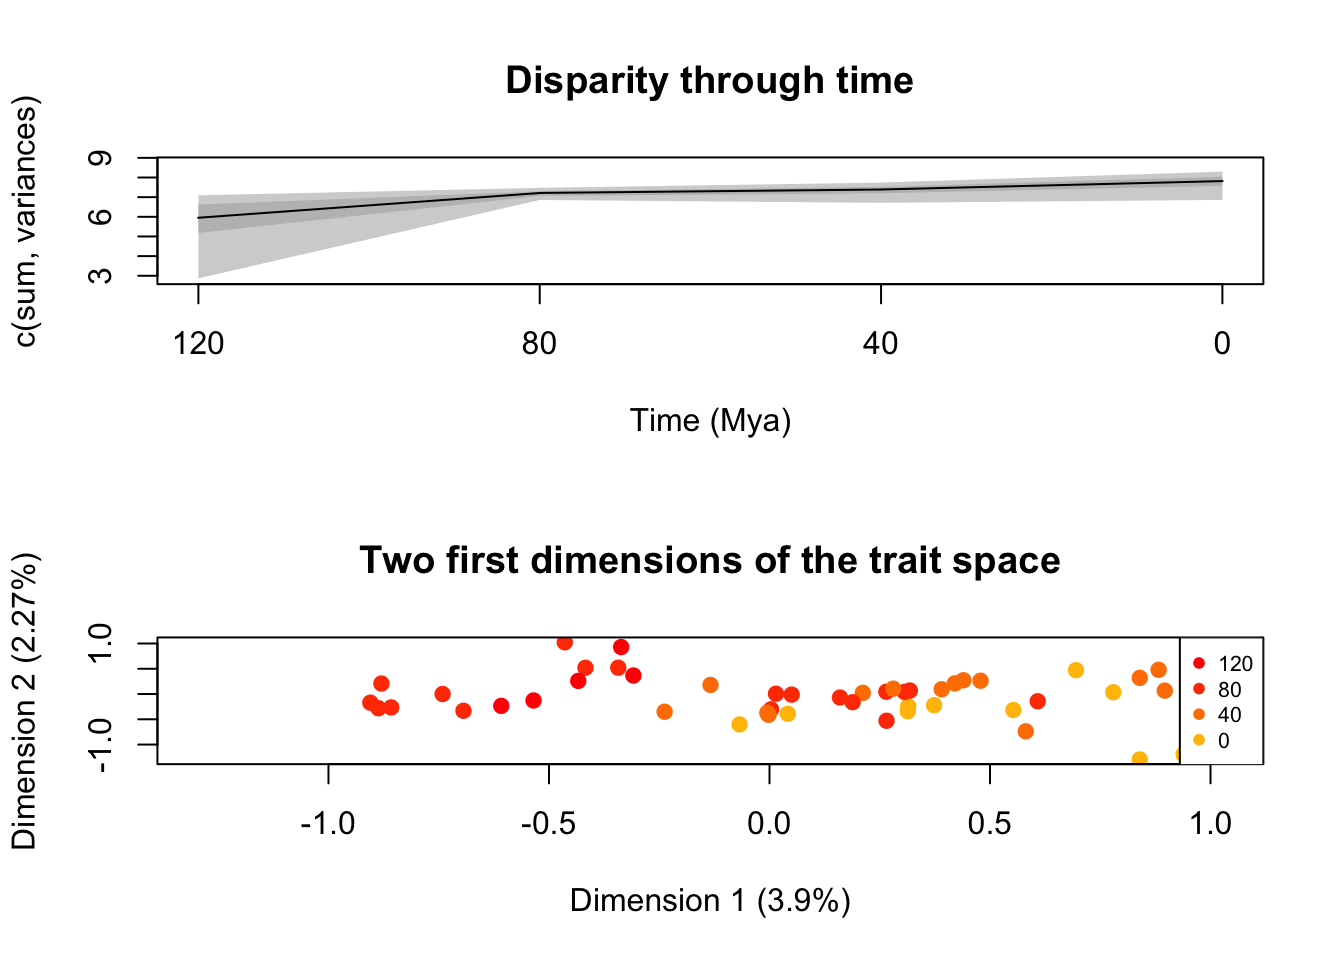
\includegraphics{dispRity_manual_files/figure-latex/unnamed-chunk-66-1.pdf}

\begin{Shaded}
\begin{Highlighting}[]
\NormalTok{## Creating doughnut space (a spherical space with a hole)}
\NormalTok{doughnut_space <-}\StringTok{ }\KeywordTok{space.maker}\NormalTok{(}\DecValTok{5000}\NormalTok{, }\DecValTok{3}\NormalTok{, }\KeywordTok{c}\NormalTok{(rnorm, random.circle),}
     \DataTypeTok{arguments =} \KeywordTok{list}\NormalTok{(}\KeywordTok{list}\NormalTok{(}\DataTypeTok{mean =} \DecValTok{0}\NormalTok{), }\KeywordTok{list}\NormalTok{(runif, }\DataTypeTok{inner =} \FloatTok{0.5}\NormalTok{, }\DataTypeTok{outer =} \DecValTok{1}\NormalTok{)))}
\end{Highlighting}
\end{Shaded}

\subsection{Visualising the space}\label{visualising-the-space}

I suggest using the excellent \texttt{scatterplot3d} package to play
around and visualise the simulated spaces:

\begin{Shaded}
\begin{Highlighting}[]
\NormalTok{## Graphical options}
\NormalTok{op <-}\StringTok{ }\KeywordTok{par}\NormalTok{(}\DataTypeTok{mfrow =}\NormalTok{ (}\KeywordTok{c}\NormalTok{(}\DecValTok{2}\NormalTok{, }\DecValTok{2}\NormalTok{)), }\DataTypeTok{bty =} \StringTok{"n"}\NormalTok{)}
\NormalTok{## Visualising 3D spaces}
\KeywordTok{require}\NormalTok{(scatterplot3d)}
\end{Highlighting}
\end{Shaded}

\begin{verbatim}
## Loading required package: scatterplot3d
\end{verbatim}

\begin{Shaded}
\begin{Highlighting}[]
\NormalTok{## The plane space}
\KeywordTok{scatterplot3d}\NormalTok{(plane_space, }\DataTypeTok{pch =} \DecValTok{20}\NormalTok{, }\DataTypeTok{xlab =} \StringTok{""}\NormalTok{, }\DataTypeTok{ylab =} \StringTok{""}\NormalTok{, }\DataTypeTok{zlab =} \StringTok{""}\NormalTok{,}
              \DataTypeTok{xlim =} \KeywordTok{c}\NormalTok{(}\OperatorTok{-}\FloatTok{0.5}\NormalTok{, }\FloatTok{0.5}\NormalTok{), }\DataTypeTok{main =} \StringTok{"Plane space"}\NormalTok{)}

\NormalTok{## The ellipsoid space}
\KeywordTok{scatterplot3d}\NormalTok{(ellipse_space, }\DataTypeTok{pch =} \DecValTok{20}\NormalTok{, }\DataTypeTok{xlab =} \StringTok{""}\NormalTok{, }\DataTypeTok{ylab =} \StringTok{""}\NormalTok{, }\DataTypeTok{zlab =} \StringTok{""}\NormalTok{,}
              \DataTypeTok{main =} \StringTok{"Normal ellipsoid space"}\NormalTok{)}

\NormalTok{## A cylindrical space with a decreasing variance per axis}
\KeywordTok{scatterplot3d}\NormalTok{(cylindrical_space, }\DataTypeTok{pch =} \DecValTok{20}\NormalTok{, }\DataTypeTok{xlab =} \StringTok{""}\NormalTok{, }\DataTypeTok{ylab =} \StringTok{""}\NormalTok{, }\DataTypeTok{zlab =} \StringTok{""}\NormalTok{,}
              \DataTypeTok{main =} \StringTok{"Normal cylindrical space"}\NormalTok{)}
\NormalTok{## Axes have different orders of magnitude}

\NormalTok{## Plotting the doughnut space}
\KeywordTok{scatterplot3d}\NormalTok{(doughnut_space[,}\KeywordTok{c}\NormalTok{(}\DecValTok{2}\NormalTok{,}\DecValTok{1}\NormalTok{,}\DecValTok{3}\NormalTok{)], }\DataTypeTok{pch =} \DecValTok{20}\NormalTok{, }\DataTypeTok{xlab =} \StringTok{""}\NormalTok{, }\DataTypeTok{ylab =} \StringTok{""}\NormalTok{,}
              \DataTypeTok{zlab =} \StringTok{""}\NormalTok{, }\DataTypeTok{main =} \StringTok{"Doughnut space"}\NormalTok{)}
\end{Highlighting}
\end{Shaded}

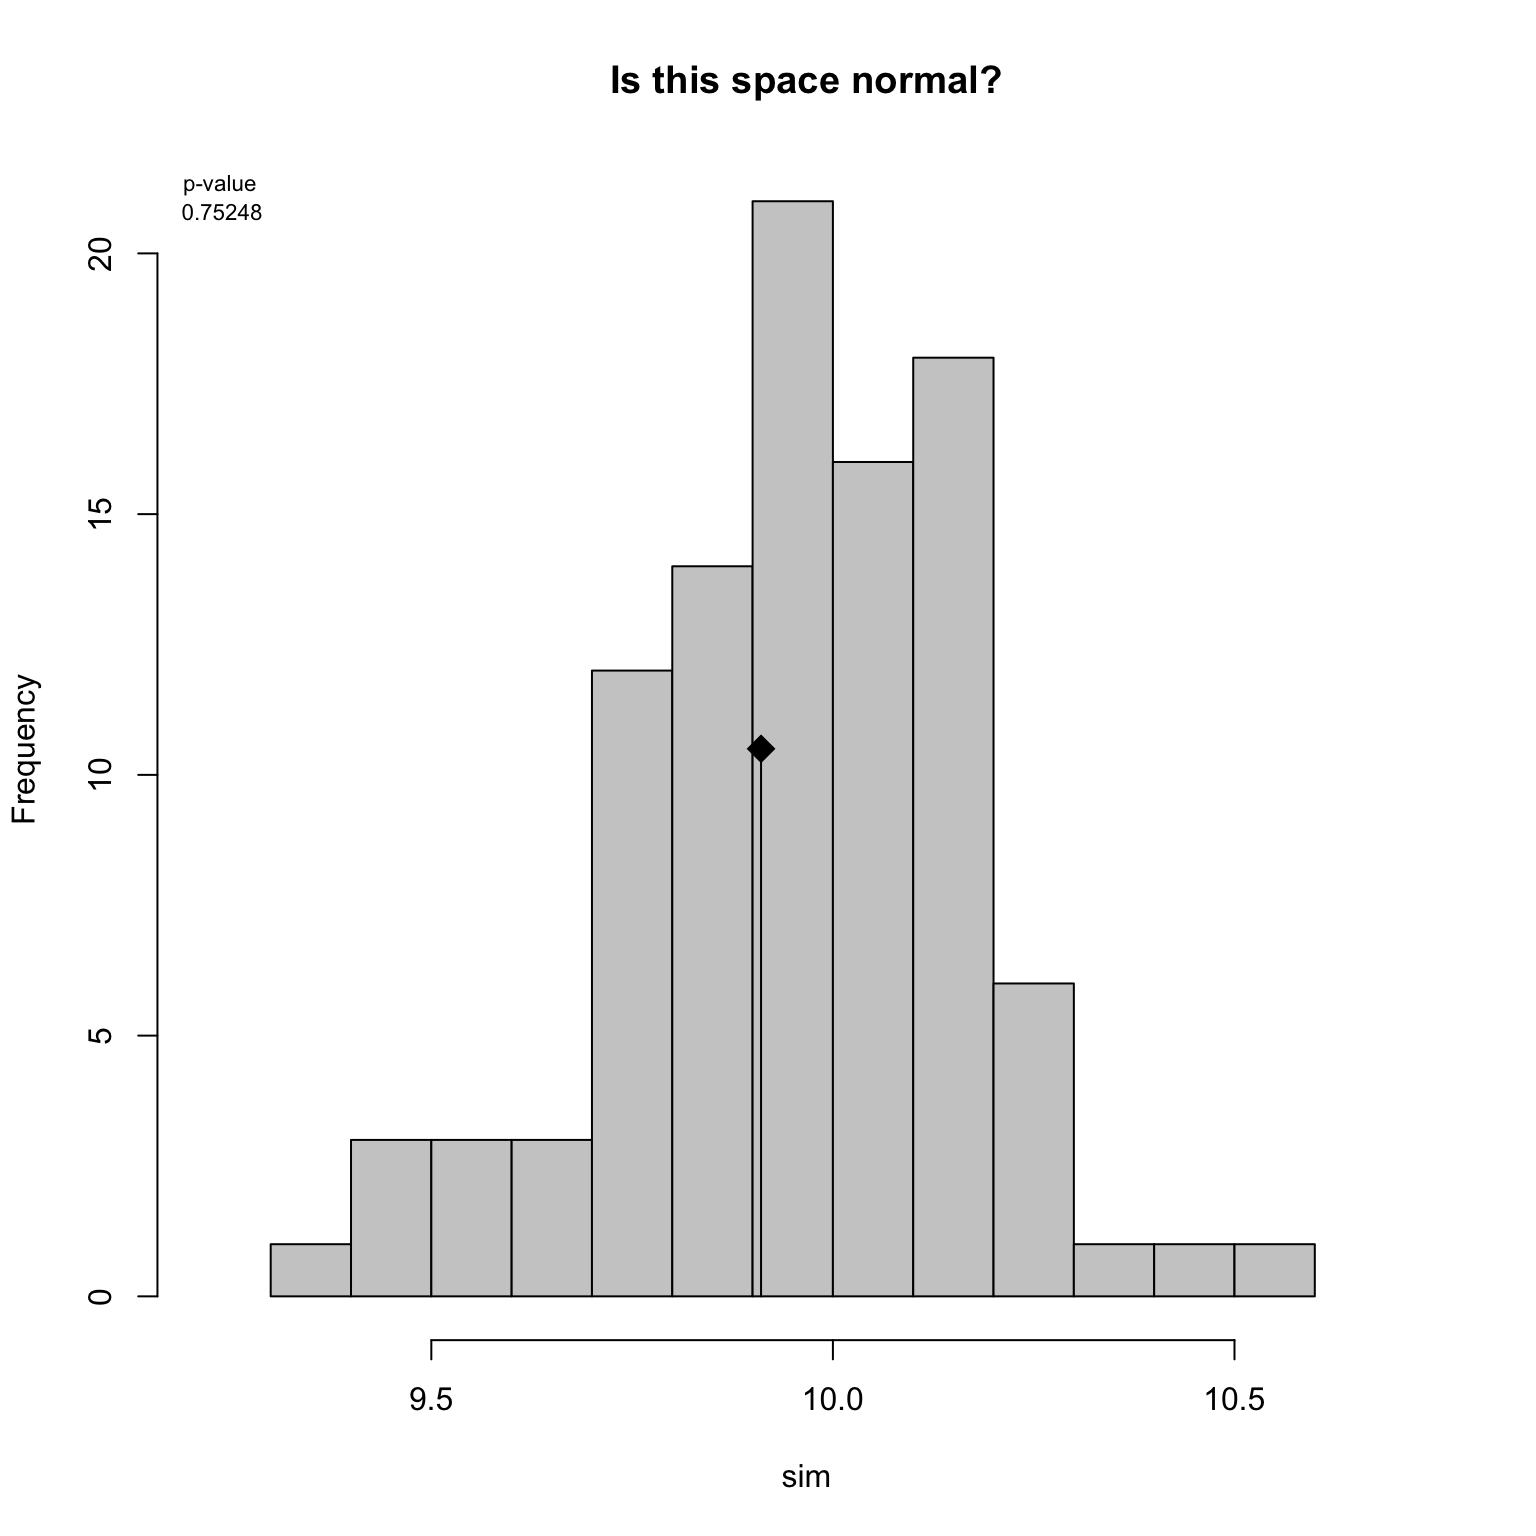
\includegraphics{dispRity_manual_files/figure-latex/unnamed-chunk-67-1.pdf}

\begin{Shaded}
\begin{Highlighting}[]
\KeywordTok{par}\NormalTok{(op)}
\end{Highlighting}
\end{Shaded}

\subsection{Generating realistic
spaces}\label{generating-realistic-spaces}

It is possible to generate ``realistic'' spaces by simply extracting the
parameters of an existing space and scaling it up to the simulated
space. For example, we can extract the parameters of the
\texttt{BeckLee\_mat50} ordinated space and simulate a similar space.

\begin{Shaded}
\begin{Highlighting}[]
\NormalTok{## Loading the data}
\KeywordTok{data}\NormalTok{(BeckLee_mat50)}

\NormalTok{## Number of dimensions}
\NormalTok{obs_dim <-}\StringTok{ }\KeywordTok{ncol}\NormalTok{(BeckLee_mat50)}

\NormalTok{## Observed correlation between the dimensions}
\NormalTok{obs_correlations <-}\StringTok{ }\KeywordTok{cor}\NormalTok{(BeckLee_mat50)}

\NormalTok{## Observed mean and standard deviation per axis}
\NormalTok{obs_mu_sd_axis <-}\StringTok{ }\KeywordTok{mapply}\NormalTok{(}\ControlFlowTok{function}\NormalTok{(x,y) }\KeywordTok{list}\NormalTok{(}\StringTok{"mean"}\NormalTok{ =}\StringTok{ }\NormalTok{x, }\StringTok{"sd"}\NormalTok{ =}\StringTok{ }\NormalTok{y),}
                         \KeywordTok{as.list}\NormalTok{(}\KeywordTok{apply}\NormalTok{(BeckLee_mat50, }\DecValTok{2}\NormalTok{, mean)),}
                         \KeywordTok{as.list}\NormalTok{(}\KeywordTok{apply}\NormalTok{(BeckLee_mat50, }\DecValTok{2}\NormalTok{, sd)), }\DataTypeTok{SIMPLIFY =} \OtherTok{FALSE}\NormalTok{)}

\NormalTok{## Observed overall mean and standard deviation}
\NormalTok{obs_mu_sd_glob <-}\StringTok{ }\KeywordTok{list}\NormalTok{(}\StringTok{"mean"}\NormalTok{ =}\StringTok{ }\KeywordTok{mean}\NormalTok{(BeckLee_mat50), }\StringTok{"sd"}\NormalTok{ =}\StringTok{ }\KeywordTok{sd}\NormalTok{(BeckLee_mat50))}

\NormalTok{## Scaled observed variance per axis (scree plot)}
\NormalTok{obs_scree <-}\StringTok{ }\KeywordTok{variances}\NormalTok{(BeckLee_mat50)}\OperatorTok{/}\KeywordTok{sum}\NormalTok{(}\KeywordTok{variances}\NormalTok{(BeckLee_mat50))}

\NormalTok{## Generating our simulated space}
\NormalTok{simulated_space <-}\StringTok{ }\KeywordTok{space.maker}\NormalTok{(}\DecValTok{1000}\NormalTok{, }\DataTypeTok{dimensions =}\NormalTok{ obs_dim, }
                               \DataTypeTok{distribution =} \KeywordTok{rep}\NormalTok{(}\KeywordTok{list}\NormalTok{(rnorm), obs_dim),}
                               \DataTypeTok{arguments =}\NormalTok{ obs_mu_sd_axis,}
                               \DataTypeTok{cor.matrix =}\NormalTok{ obs_correlations)}

\NormalTok{## Visualising the fit of our data in the space (in the two first dimensions)}
\KeywordTok{plot}\NormalTok{(simulated_space[,}\DecValTok{1}\OperatorTok{:}\DecValTok{2}\NormalTok{], }\DataTypeTok{xlab =} \StringTok{"PC1"}\NormalTok{, }\DataTypeTok{ylab =} \StringTok{"PC2"}\NormalTok{)}
\KeywordTok{points}\NormalTok{(BeckLee_mat50[,}\DecValTok{1}\OperatorTok{:}\DecValTok{2}\NormalTok{], }\DataTypeTok{col =} \StringTok{"red"}\NormalTok{, }\DataTypeTok{pch =} \DecValTok{20}\NormalTok{)}
\KeywordTok{legend}\NormalTok{(}\StringTok{"topleft"}\NormalTok{, }\DataTypeTok{legend =} \KeywordTok{c}\NormalTok{(}\StringTok{"observed"}\NormalTok{, }\StringTok{"simulated"}\NormalTok{),}
        \DataTypeTok{pch =} \KeywordTok{c}\NormalTok{(}\DecValTok{20}\NormalTok{,}\DecValTok{21}\NormalTok{), }\DataTypeTok{col =} \KeywordTok{c}\NormalTok{(}\StringTok{"red"}\NormalTok{, }\StringTok{"black"}\NormalTok{))}
\end{Highlighting}
\end{Shaded}

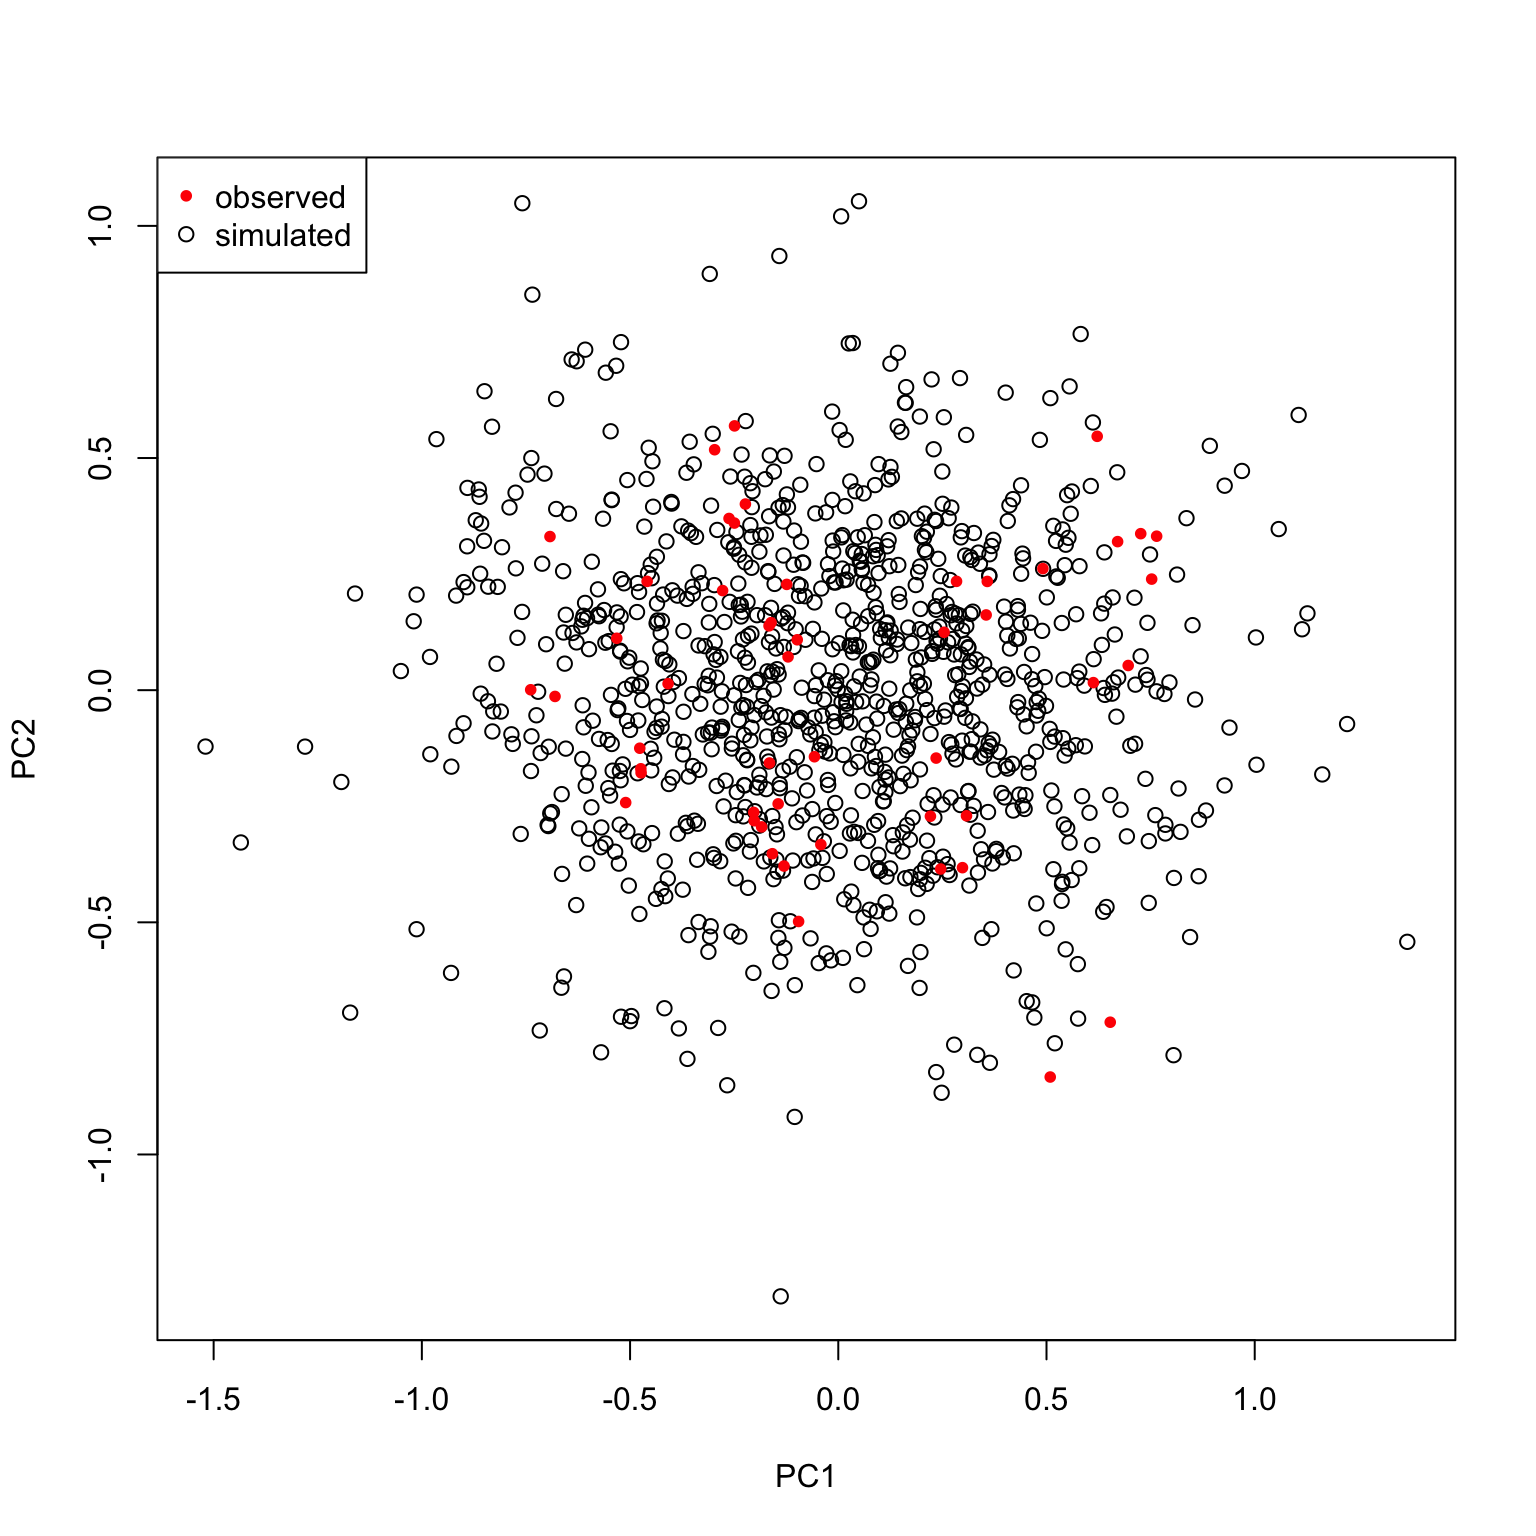
\includegraphics{dispRity_manual_files/figure-latex/unnamed-chunk-68-1.pdf}

It is now possible to simulate a space using these observed arguments to
test several hypothesis:

\begin{itemize}
\tightlist
\item
  Is the space uniform or normal?
\item
  If the space is normal, is the mean and variance global or specific
  for each axis?
\end{itemize}

\begin{Shaded}
\begin{Highlighting}[]
\NormalTok{## Measuring disparity as the sum of variance}
\NormalTok{observed_disp <-}\StringTok{ }\KeywordTok{dispRity}\NormalTok{(BeckLee_mat50, }\DataTypeTok{metric =} \KeywordTok{c}\NormalTok{(median, centroids))}

\NormalTok{## Is the space uniform?}
\NormalTok{test_unif <-}\StringTok{ }\KeywordTok{null.test}\NormalTok{(observed_disp, }\DataTypeTok{null.distrib =}\NormalTok{ runif)}

\NormalTok{## Is the space normal with a mean of 0 and a sd of 1?}
\NormalTok{test_norm1 <-}\StringTok{ }\KeywordTok{null.test}\NormalTok{(observed_disp, }\DataTypeTok{null.distrib =}\NormalTok{ rnorm)}

\NormalTok{## Is the space normal with the observed mean and sd and cumulative variance}
\NormalTok{test_norm2 <-}\StringTok{ }\KeywordTok{null.test}\NormalTok{(observed_disp, }\DataTypeTok{null.distrib =} \KeywordTok{rep}\NormalTok{(}\KeywordTok{list}\NormalTok{(rnorm), obs_dim),}
                        \DataTypeTok{null.args =} \KeywordTok{rep}\NormalTok{(}\KeywordTok{list}\NormalTok{(obs_mu_sd_glob), obs_dim),}
                        \DataTypeTok{null.scree =}\NormalTok{ obs_scree)}

\NormalTok{## Is the space multiple normal with multiple means and sds and a correlation?}
\NormalTok{test_norm3 <-}\StringTok{ }\KeywordTok{null.test}\NormalTok{(observed_disp, }\DataTypeTok{null.distrib =} \KeywordTok{rep}\NormalTok{(}\KeywordTok{list}\NormalTok{(rnorm), obs_dim),}
                        \DataTypeTok{null.args =}\NormalTok{ obs_mu_sd_axis, }\DataTypeTok{null.cor =}\NormalTok{ obs_correlations)}


\NormalTok{## Graphical options}
\NormalTok{op <-}\StringTok{ }\KeywordTok{par}\NormalTok{(}\DataTypeTok{mfrow =}\NormalTok{ (}\KeywordTok{c}\NormalTok{(}\DecValTok{2}\NormalTok{, }\DecValTok{2}\NormalTok{)), }\DataTypeTok{bty =} \StringTok{"n"}\NormalTok{)}
\NormalTok{## Plotting the results}
\KeywordTok{plot}\NormalTok{(test_unif, }\DataTypeTok{main =} \StringTok{"Uniform (0,1)"}\NormalTok{)}
\KeywordTok{plot}\NormalTok{(test_norm1, }\DataTypeTok{main =} \StringTok{"Normal (0,1)"}\NormalTok{)}
\KeywordTok{plot}\NormalTok{(test_norm2, }\DataTypeTok{main =} \KeywordTok{paste0}\NormalTok{(}\StringTok{"Normal ("}\NormalTok{, }\KeywordTok{round}\NormalTok{(obs_mu_sd_glob[[}\DecValTok{1}\NormalTok{]], }\DataTypeTok{digit =} \DecValTok{3}\NormalTok{),}
                              \StringTok{","}\NormalTok{, }\KeywordTok{round}\NormalTok{(obs_mu_sd_glob[[}\DecValTok{2}\NormalTok{]], }\DataTypeTok{digit =} \DecValTok{3}\NormalTok{), }\StringTok{")"}\NormalTok{))}
\KeywordTok{plot}\NormalTok{(test_norm3, }\DataTypeTok{main =} \StringTok{"Normal (variable + correlation)"}\NormalTok{)}
\end{Highlighting}
\end{Shaded}

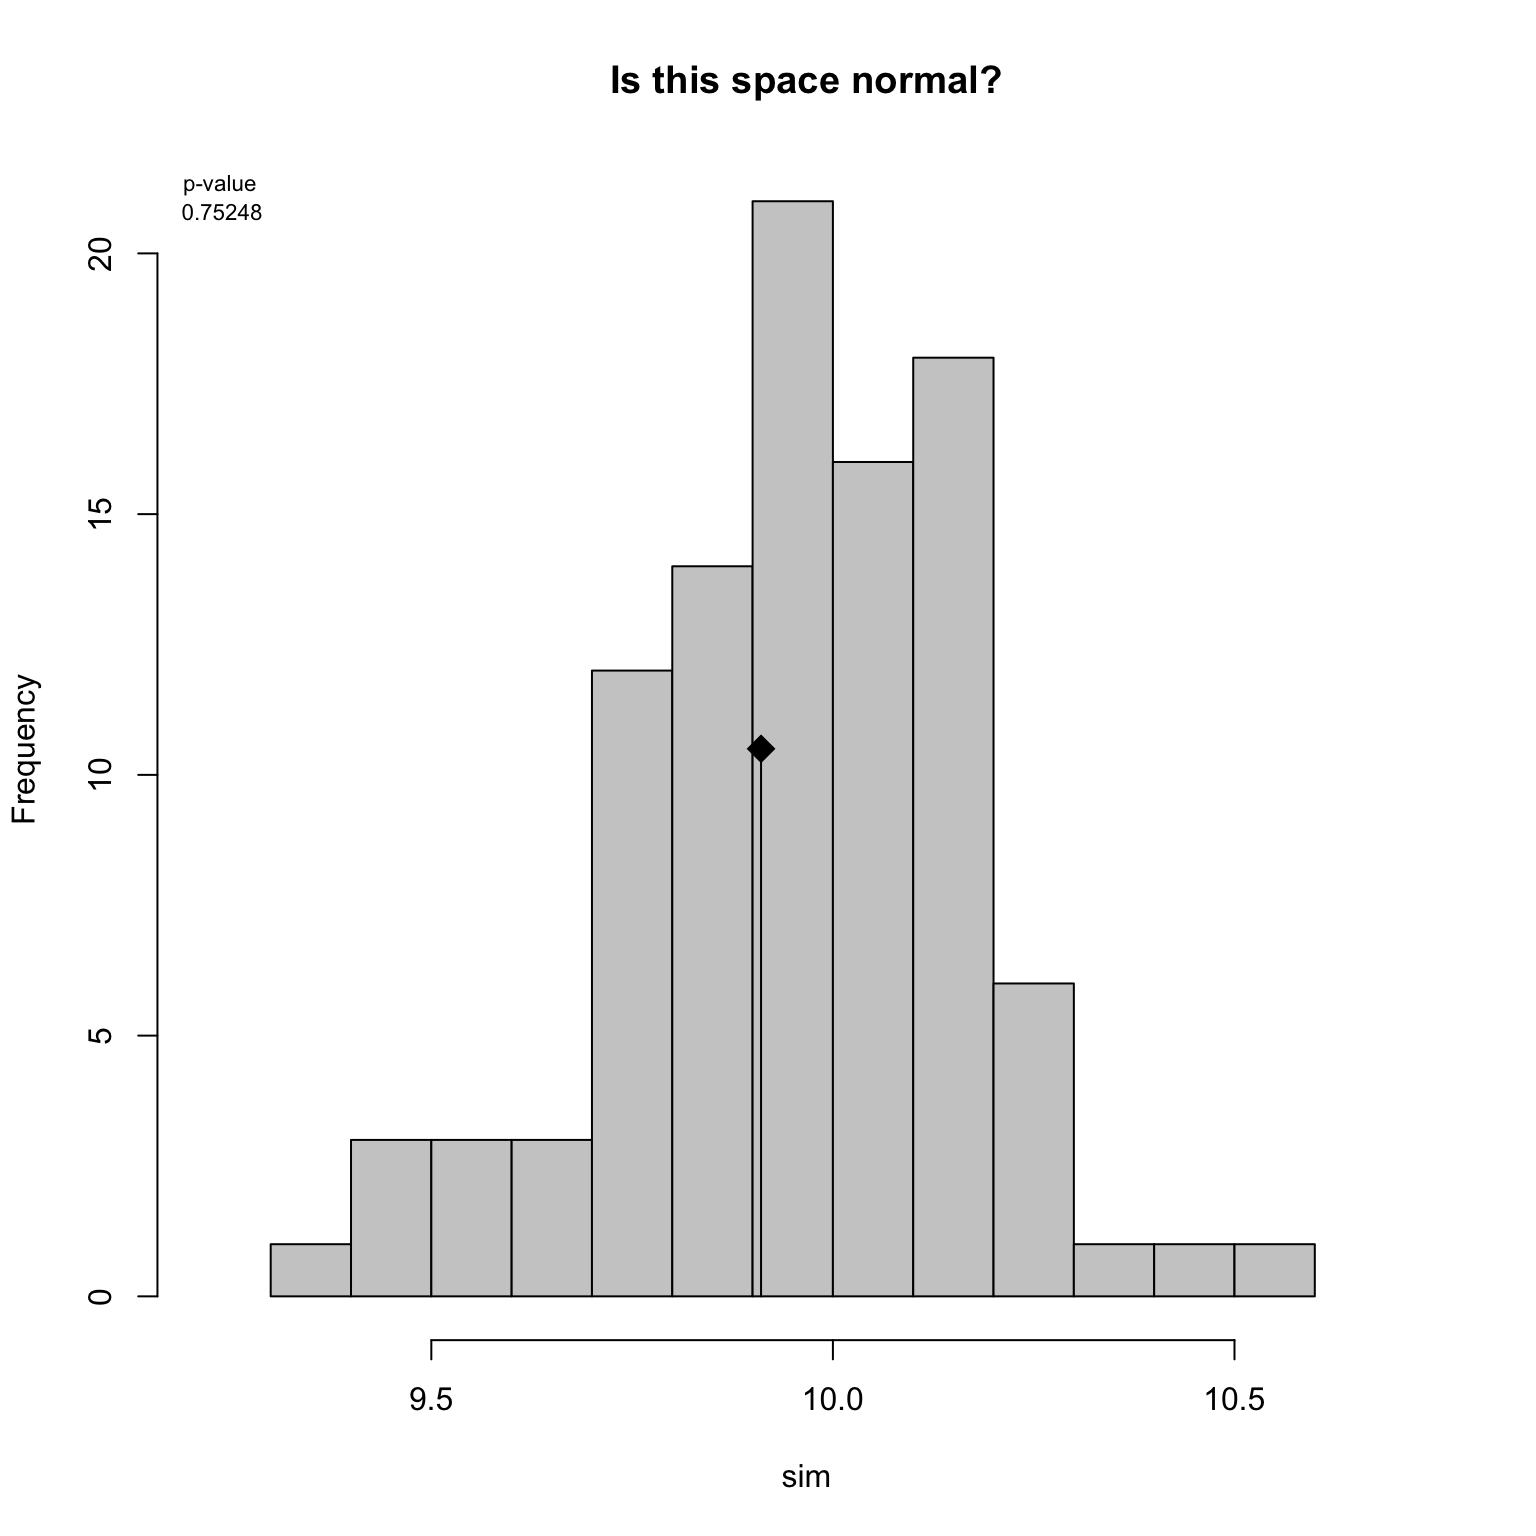
\includegraphics{dispRity_manual_files/figure-latex/unnamed-chunk-69-1.pdf}

If we measure disparity as the median distance from the morphospace
centroid, we can explain the distribution of the data as normal with the
variable observed mean and standard deviation and with a correlation
between the dimensions.

\chapter{\texorpdfstring{The guts of the \texttt{dispRity}
package}{The guts of the dispRity package}}\label{the-guts-of-the-disprity-package}

\section{\texorpdfstring{Manipulating \texttt{dispRity}
objects}{Manipulating dispRity objects}}\label{manipulating-disprity-objects}

Disparity analysis involves a lot of manipulation of many matrices
(especially when bootstrapping) which can be impractical to visualise
and will quickly overwhelm your \texttt{R} console. Even the simple Beck
and Lee 2014 example above produces an object with \textgreater{} 72
lines of lists of lists of matrices!

Therefore \texttt{dispRity} uses a specific class of object called a
\texttt{dispRity} object. These objects allow users to use S3 method
functions such as \texttt{summary.dispRity}, \texttt{plot.dispRity} and
\texttt{print.dispRity}. \texttt{dispRity} also contains various utility
functions that manipulate the \texttt{dispRity} object (e.g.
\texttt{sort.dispRity}, \texttt{extract.dispRity} see the full list in
the next section). These functions modify the \texttt{dispRity} object
without having to delve into its complex structure! The full structure
of a \texttt{dispRity} object is detailed
\href{https://github.com/TGuillerme/dispRity/blob/master/disparity_object.md}{here}.

\begin{Shaded}
\begin{Highlighting}[]
\NormalTok{## Loading the example data}
\KeywordTok{data}\NormalTok{(disparity)}

\NormalTok{## What is the class of the median_centroids object?}
\KeywordTok{class}\NormalTok{(disparity)}
\end{Highlighting}
\end{Shaded}

\begin{verbatim}
## [1] "dispRity"
\end{verbatim}

\begin{Shaded}
\begin{Highlighting}[]
\NormalTok{## What does the object contain?}
\KeywordTok{names}\NormalTok{(disparity)}
\end{Highlighting}
\end{Shaded}

\begin{verbatim}
## [1] "matrix"     "call"       "subsamples" "disparity"
\end{verbatim}

\begin{Shaded}
\begin{Highlighting}[]
\NormalTok{## Summarising it using the S3 method print.dispRity}
\NormalTok{disparity}
\end{Highlighting}
\end{Shaded}

\begin{verbatim}
##  ---- dispRity object ---- 
## 7 continuous (acctran) time subsamples for 99 elements with 97 dimensions:
##      90, 80, 70, 60, 50 ...
## Data was bootstrapped 100 times (method:"full") and rarefied to 20, 15, 10, 5 elements.
## Disparity was calculated as: c(median, centroids).
\end{verbatim}

Note that it is always possible to recall the full object using the
argument \texttt{all\ =\ TRUE} in \texttt{print.dispRity}:

\begin{Shaded}
\begin{Highlighting}[]
\NormalTok{## Display the full object}
\KeywordTok{print}\NormalTok{(disparity, }\DataTypeTok{all =} \OtherTok{TRUE}\NormalTok{)}
\NormalTok{## This is more nearly ~ 5000 lines on my 13 inch laptop screen!}
\end{Highlighting}
\end{Shaded}

\section{\texorpdfstring{\texttt{dispRity}
utilities}{dispRity utilities}}\label{disprity-utilities}

The package also provides some utility functions to facilitate
multidimensional analysis.

\subsection{\texorpdfstring{\texttt{dispRity} object utilities
}{dispRity object utilities }}\label{disprity-object-utilities}

The first set of utilities are functions for manipulating
\texttt{dispRity} objects:

\subsubsection{\texorpdfstring{\texttt{make.dispRity}}{make.dispRity}}\label{make.disprity}

This function creates empty \texttt{dispRity} objects.

\begin{Shaded}
\begin{Highlighting}[]
\NormalTok{## Creating an empty dispRity object}
\KeywordTok{make.dispRity}\NormalTok{()}
\end{Highlighting}
\end{Shaded}

\begin{verbatim}
## Empty dispRity object.
\end{verbatim}

\begin{Shaded}
\begin{Highlighting}[]
\NormalTok{## Creating an "empty" dispRity object with a matrix}
\NormalTok{(disparity_obj <-}\StringTok{ }\KeywordTok{make.dispRity}\NormalTok{(}\KeywordTok{matrix}\NormalTok{(}\KeywordTok{rnorm}\NormalTok{(}\DecValTok{20}\NormalTok{), }\DecValTok{5}\NormalTok{, }\DecValTok{4}\NormalTok{)))}
\end{Highlighting}
\end{Shaded}

\begin{verbatim}
##  ---- dispRity object ---- 
## Contains only a matrix 5x4.
\end{verbatim}

\subsubsection{\texorpdfstring{\texttt{fill.dispRity}}{fill.dispRity}}\label{fill.disprity}

This function initialises a \texttt{dispRity} object and generates its
call properties.

\begin{Shaded}
\begin{Highlighting}[]
\NormalTok{## The dispRity object's call is indeed empty}
\NormalTok{disparity_obj}\OperatorTok{$}\NormalTok{call}
\end{Highlighting}
\end{Shaded}

\begin{verbatim}
## list()
\end{verbatim}

\begin{Shaded}
\begin{Highlighting}[]
\NormalTok{## Filling an empty disparity object (that needs to contain at least a matrix)}
\NormalTok{(disparity_obj <-}\StringTok{ }\KeywordTok{fill.dispRity}\NormalTok{(disparity_obj))}
\end{Highlighting}
\end{Shaded}

\begin{verbatim}
##  ---- dispRity object ---- 
## 5 elements with 4 dimensions.
\end{verbatim}

\begin{Shaded}
\begin{Highlighting}[]
\NormalTok{## The dipRity object has now the correct minimal attributes}
\NormalTok{disparity_obj}\OperatorTok{$}\NormalTok{call}
\end{Highlighting}
\end{Shaded}

\begin{verbatim}
## $dimensions
## [1] 4
\end{verbatim}

\subsubsection{\texorpdfstring{\texttt{matrix.dispRity}}{matrix.dispRity}}\label{matrix.disprity}

This function extracts a specific matrix from a disparity object. The
matrix can be one of the bootstrapped matrices or/and a rarefied matrix.

\begin{Shaded}
\begin{Highlighting}[]
\NormalTok{## Extracting the matrix containing the coordinates of the elements at time 50}
\KeywordTok{str}\NormalTok{(}\KeywordTok{matrix.dispRity}\NormalTok{(disparity, }\StringTok{"50"}\NormalTok{))}
\end{Highlighting}
\end{Shaded}

\begin{verbatim}
##  num [1:18, 1:97] -0.1038 0.2844 0.2848 0.0927 0.1619 ...
##  - attr(*, "dimnames")=List of 2
##   ..$ : chr [1:18] "Leptictis" "Dasypodidae" "n24" "Potamogalinae" ...
##   ..$ : NULL
\end{verbatim}

\begin{Shaded}
\begin{Highlighting}[]
\NormalTok{## Extracting the 3rd bootstrapped matrix with the 2nd rarefaction level}
\NormalTok{## (15 elements) from the second group (80 Mya)}
\KeywordTok{str}\NormalTok{(}\KeywordTok{matrix.dispRity}\NormalTok{(disparity, }\DataTypeTok{subsamples =} \DecValTok{1}\NormalTok{, }\DataTypeTok{bootstrap =} \DecValTok{3}\NormalTok{, }\DataTypeTok{rarefaction =} \DecValTok{2}\NormalTok{))}
\end{Highlighting}
\end{Shaded}

\begin{verbatim}
##  num [1:15, 1:97] -0.7161 0.3496 -0.573 -0.0445 -0.1427 ...
##  - attr(*, "dimnames")=List of 2
##   ..$ : chr [1:15] "n7" "n34" "Maelestes" "n20" ...
##   ..$ : NULL
\end{verbatim}

\subsubsection{\texorpdfstring{\texttt{get.subsamples.dispRity}}{get.subsamples.dispRity}}\label{get.subsamples.disprity}

This function creates a dispRity object that contains only elements from
one specific subsamples.

\begin{Shaded}
\begin{Highlighting}[]
\NormalTok{## Extracting all the data for the crown mammals}
\NormalTok{(crown_mammals <-}\StringTok{ }\KeywordTok{get.subsamples.dispRity}\NormalTok{(disp_crown_stemBS, }\StringTok{"Group.crown"}\NormalTok{))}

\NormalTok{## The object keeps the properties of the parent object but is composed of only one subsamples}
\KeywordTok{length}\NormalTok{(crown_mammals}\OperatorTok{$}\NormalTok{subsamples)}
\end{Highlighting}
\end{Shaded}

\subsubsection{\texorpdfstring{\texttt{extract.dispRity}}{extract.dispRity}}\label{extract.disprity}

This function extracts the calculated disparity values of a specific
matrix.

\begin{Shaded}
\begin{Highlighting}[]
\NormalTok{## Extracting the observed disparity (default)}
\KeywordTok{extract.dispRity}\NormalTok{(disparity)}

\NormalTok{## Extracting the disparity from the bootstrapped values from the}
\NormalTok{## 10th rarefaction level from the second subsamples (80 Mya)}
\KeywordTok{extract.dispRity}\NormalTok{(disparity, }\DataTypeTok{observed =} \OtherTok{FALSE}\NormalTok{, }\DataTypeTok{subsamples =} \DecValTok{2}\NormalTok{, }\DataTypeTok{rarefaction =} \DecValTok{10}\NormalTok{)}
\end{Highlighting}
\end{Shaded}

\subsubsection{\texorpdfstring{\texttt{scale.dispRity}}{scale.dispRity}}\label{scale.disprity}

This is the S3 method of \texttt{scale} (scaling and/or centring) that
can be applied to the disparity data of a \texttt{dispRity} object.

\begin{Shaded}
\begin{Highlighting}[]
\NormalTok{## Getting the disparity values of the time subsamples}
\KeywordTok{head}\NormalTok{(}\KeywordTok{summary}\NormalTok{(disparity))}

\NormalTok{## Scaling the same disparity values}
\KeywordTok{head}\NormalTok{(}\KeywordTok{summary}\NormalTok{(}\KeywordTok{scale}\NormalTok{(disparity, }\DataTypeTok{scale =} \OtherTok{TRUE}\NormalTok{)))}

\NormalTok{## Scaling and centering:}
\KeywordTok{head}\NormalTok{(}\KeywordTok{summary}\NormalTok{(}\KeywordTok{scale}\NormalTok{(disparity, }\DataTypeTok{scale =} \OtherTok{TRUE}\NormalTok{, }\DataTypeTok{center =} \OtherTok{TRUE}\NormalTok{)))}
\end{Highlighting}
\end{Shaded}

\subsubsection{\texorpdfstring{\texttt{sort.dispRity}}{sort.dispRity}}\label{sort.disprity}

This is the S3 method of \texttt{sort} for sorting the subsamples
alphabetically (default) or following a specific pattern.

\begin{Shaded}
\begin{Highlighting}[]
\NormalTok{## Sorting the disparity subsamples in inverse alphabetic order}
\KeywordTok{head}\NormalTok{(}\KeywordTok{summary}\NormalTok{(}\KeywordTok{sort}\NormalTok{(disparity, }\DataTypeTok{decreasing =} \OtherTok{TRUE}\NormalTok{)))}

\NormalTok{## Customised sorting}
\KeywordTok{head}\NormalTok{(}\KeywordTok{summary}\NormalTok{(}\KeywordTok{sort}\NormalTok{(disparity, }\DataTypeTok{sort =} \KeywordTok{c}\NormalTok{(}\DecValTok{7}\NormalTok{, }\DecValTok{1}\NormalTok{, }\DecValTok{3}\NormalTok{, }\DecValTok{4}\NormalTok{, }\DecValTok{5}\NormalTok{, }\DecValTok{2}\NormalTok{, }\DecValTok{6}\NormalTok{))))}
\end{Highlighting}
\end{Shaded}

\section{\texorpdfstring{The \texttt{dispRity} object
content}{The dispRity object content}}\label{the-disprity-object-content}

The functions above are utilities to easily and safely access different
elements in the \texttt{dispRity} object. Alternatively, of course, each
elements can be accessed manually. Here is an explanation on how it
works. The \texttt{dispRity} object is a \texttt{list} of two to four
elements, each of which are detailed below:

\begin{itemize}
\tightlist
\item
  \texttt{\$matrix}: an object of class \texttt{matrix}, the full
  multidimensional space.
\item
  \texttt{\$call}: an object of class \texttt{list} containing
  information on the \texttt{dispRity} object content.
\item
  \texttt{\$subsamples}: an object of class \texttt{list} containing the
  subsamples of the multidimensional space.
\item
  \texttt{\$disparity}: an object of class \texttt{list} containing the
  disparity values.
\end{itemize}

The \texttt{dispRity} object is loosely based on \texttt{C} structure
objects. In fact, it is composed of one unique instance of a matrix (the
multidimensional space) upon which the metric function is called via
``pointers'' to only a certain number of elements and/or dimensions of
this matrix. This allows for: (1) faster and easily tractable execution
time: the metric functions are called through apply family function and
can be parallelised; and (2) a really low memory footprint: at any time,
only one matrix is present in the \texttt{R} environment rather than
multiple copies of it for each subsample.

\subsection{\texorpdfstring{\texttt{\$matrix}}{\$matrix}}\label{matrix}

This is the multidimensional space, stored in the \texttt{R} environment
as a \texttt{matrix} object. It requires row names but not column names.
By default, if the row names are missing, \texttt{dispRity} function
will arbitrarily generate them in numeric order (i.e.
\texttt{rownames(matrix)\ \textless{}-\ 1:nrow(matrix)}). This element
of the \texttt{dispRity} object is never modified.

\subsection{\texorpdfstring{\texttt{\$call}}{\$call}}\label{call}

This element contains the information on the \texttt{dispRity} object
content. It is a \texttt{list} that can contain the following:

\begin{itemize}
\tightlist
\item
  \texttt{\$call\$subsamples}: a vector of \texttt{character} with
  information on the subsamples type (either \texttt{"continuous"},
  \texttt{"discrete"} or \texttt{"custom"}) and their eventual model
  (\texttt{"acctran"}, \texttt{"deltran"}, \texttt{"punctuated"},
  \texttt{"gradual"}). This element generated only once via
  \texttt{time.subsamples()} and \texttt{custom.subsamples()}.
\item
  \texttt{\$call\$dimensions}: either a single \texttt{numeric} value
  indicating how many dimensions to use or a vector of \texttt{numeric}
  values indicating which specific dimensions to use. This element is by
  default the number of columns in \texttt{\$matrix} but can be modified
  through \texttt{boot.matrix()} or \texttt{dispRity()}.
\item
  \texttt{\$call\$bootstrap}: this is a \texttt{list} containing three
  elements:

  \begin{itemize}
  \tightlist
  \item
    \texttt{{[}{[}1{]}{]}}: the number of bootstrap replicates
    (\texttt{numeric})
  \item
    \texttt{{[}{[}2{]}{]}}: the bootstrap method (\texttt{character})
  \item
    \texttt{{[}{[}3{]}{]}}: the rarefaction levels (\texttt{numeric}
    vector)
  \end{itemize}
\item
  \texttt{\$call\$disparity}: this is a \texttt{list} containing one
  element, \texttt{\$metric}, that is a \texttt{list} containing the
  different functions passed to the \texttt{metric} argument in
  \texttt{dispRity}. These are \texttt{call} elements and get modified
  each time the \texttt{dispRity} function is used (the first element is
  the first metric(s), the second, the second metric(s), etc.).
\end{itemize}

\subsection{\texorpdfstring{\texttt{\$subsamples}}{\$subsamples}}\label{subsamples}

This element contain the eventual subsamples of the multidimensional
space. It is a \texttt{list} of subsample names. Each subsample name is
in turn a \texttt{list} of at least one element called \texttt{elements}
which is in turn a \texttt{matrix}. This \texttt{elements} matrix is the
raw (observed) elements in the subsamples. The \texttt{elements} matrix
is composed of \texttt{numeric} values in one column and \emph{n} rows
(the number of elements in the subsample). Each of these values are a
``pointer'' (\texttt{C} inspired) to the element of the
\texttt{\$matrix}. For example, lets assume a \texttt{dispRity} object
called \texttt{disparity}, composed of at least one subsamples called
\texttt{sub1}:

\begin{verbatim}
 disparity$subsamples$sub1$elements
      [,1]
 [1,]    5
 [2,]    4
 [3,]    6
 [4,]    7
\end{verbatim}

The values in the matrix ``point'' to the elements in \texttt{\$matrix}:
here, the multidimensional space with only the 4th, 5th, 6th and 7th
elements. The following elements in \texttt{diparity\$subsamples\$sub1}
will correspond to the same ``pointers'' but drawn from the bootstrap
replicates. The columns will correspond to different bootstrap
replicates. For example:

\begin{verbatim}
 disparity$subsamples$sub1[[2]]
      [,1] [,2] [,3] [,4]
 [1,]   57   43   70    4
 [2,]   43   44    4    4
 [3,]   42   84   44    1
 [4,]   84    7    2   10
\end{verbatim}

This signifies that we have four bootstrap pseudo-replicates pointing
each time to four elements in \texttt{\$matrix}. The next element
(\texttt{{[}{[}3{]}{]}}) will be the same for the eventual first
rarefaction level (i.e.~the resulting bootstrap matrix will have
\emph{m} rows where \emph{m} is the number of elements for this
rarefaction level). The next element after that (\texttt{{[}{[}4{]}{]}})
will be the same for with an other rarefaction level and so
forth\ldots{}

\subsection{\texorpdfstring{\texttt{\$disparity}}{\$disparity}}\label{disparity}

The \texttt{\$disparity} element is identical to the
\texttt{\$subsamples} element structure (a list of list(s) containing
matrices) but the matrices don't contain ``pointers'' to
\texttt{\$matrix} but the disparity result of the disparity metric
applied to the ``pointers''. For example, in our first example
(\texttt{\$elements}) from above, if the disparity metric is of
dimensions level 1, we would have:

\begin{verbatim}
 disparity$disparity$sub1$elements
      [,1]
 [1,]    1.82
\end{verbatim}

This is the observed disparity (1.82) for the subsample called
\texttt{sub1}. If the disparity metric is of dimension level 2 (say the
function \texttt{range} that outputs two values), we would have:

\begin{verbatim}
 disparity$disparity$sub1$elements
      [,1]
 [1,]    0.82
 [2,]    2.82
\end{verbatim}

The following elements in the list follow the same logic as before: rows
are disparity values (one row for a dimension level 1 metric, multiple
for a dimensions level 2 metric) and columns are the bootstrap
replicates (the bootstrap with all elements followed by the eventual
rarefaction levels). For example for the bootstrap without rarefaction
(second element of the list):

\begin{verbatim}
 disparity$disparity$sub1[[2]]
         [,1]     [,2]     [,3]     [,4]
[1,] 1.744668 1.777418 1.781624 1.739679 
\end{verbatim}

\chapter{Palaeobiology demo: disparity-through-time and within
groups}\label{palaeobiology-demo-disparity-through-time-and-within-groups}

This demo aims to give quick overview of the \texttt{dispRity} package
(v.0.4) for palaeobiology analyses of disparity, including disparity
through time analyses.

This demo showcases a typical disparity-through-time analysis: we are
going to test whether the disparity changed through time in a subset of
eutherian mammals from the last 100 million years using a dataset from
Beck and Lee (2014).

\section{Before starting}\label{before-starting}

\subsection{The morphospace}\label{the-morphospace}

In this example, we are going to use a subset of the data from Beck and
Lee (2014). See the \protect\hyperlink{example-data}{example data}
description for more details. Briefly, this dataset contains an
ordinated matrix of 50 discrete characters from mammals
(\texttt{BeckLee\_mat50}), another matrix of the same 50 mammals and the
estimated discrete data characters of their descendants (thus 50 + 49
rows, \texttt{BeckLee\_mat99}), a dataframe containing the ages of each
taxon in the dataset (\texttt{BeckLee\_ages}) and finally a phylogenetic
tree with the relationships among the 50 mammals
(\texttt{BeckLee\_tree}). The ordinated matrix will represent our full
morphospace, i.e.~all the mammalian morphologies that ever existed
through time (for this dataset).

\begin{Shaded}
\begin{Highlighting}[]
\NormalTok{## Loading demo and the package data}
\KeywordTok{library}\NormalTok{(dispRity)}

\NormalTok{## Setting the random seed for repeatability}
\KeywordTok{set.seed}\NormalTok{(}\DecValTok{123}\NormalTok{)}

\NormalTok{## Loading the ordinated matrix/morphospace:}
\KeywordTok{data}\NormalTok{(BeckLee_mat50)}
\KeywordTok{head}\NormalTok{(BeckLee_mat50[,}\DecValTok{1}\OperatorTok{:}\DecValTok{5}\NormalTok{])}
\end{Highlighting}
\end{Shaded}

\begin{verbatim}
##                    [,1]          [,2]        [,3]       [,4]      [,5]
## Cimolestes   -0.5319679  0.1117759259  0.09865194 -0.1933148 0.2035833
## Maelestes    -0.4087147  0.0139690317  0.26268300  0.2297096 0.1310953
## Batodon      -0.6923194  0.3308625215 -0.10175223 -0.1899656 0.1003108
## Bulaklestes  -0.6802291 -0.0134872777  0.11018009 -0.4103588 0.4326298
## Daulestes    -0.7386111  0.0009001369  0.12006449 -0.4978191 0.4741342
## Uchkudukodon -0.5105254 -0.2420633915  0.44170317 -0.1172972 0.3602273
\end{verbatim}

\begin{Shaded}
\begin{Highlighting}[]
\KeywordTok{dim}\NormalTok{(BeckLee_mat50)}
\end{Highlighting}
\end{Shaded}

\begin{verbatim}
## [1] 50 48
\end{verbatim}

\begin{Shaded}
\begin{Highlighting}[]
\NormalTok{## The morphospace contains 50 taxa and has 48 dimensions (or axes)}

\NormalTok{## Showing a list of first and last occurrences data for some fossils}
\KeywordTok{data}\NormalTok{(BeckLee_ages)}
\KeywordTok{head}\NormalTok{(BeckLee_ages)}
\end{Highlighting}
\end{Shaded}

\begin{verbatim}
##             FAD  LAD
## Adapis     37.2 36.8
## Asioryctes 83.6 72.1
## Leptictis  33.9 33.3
## Miacis     49.0 46.7
## Mimotona   61.6 59.2
## Notharctus 50.2 47.0
\end{verbatim}

\begin{Shaded}
\begin{Highlighting}[]
\NormalTok{## Plotting a phylogeny}
\KeywordTok{data}\NormalTok{(BeckLee_tree)}
\KeywordTok{plot}\NormalTok{(BeckLee_tree, }\DataTypeTok{cex =} \FloatTok{0.7}\NormalTok{)}
\KeywordTok{axisPhylo}\NormalTok{(}\DataTypeTok{root =} \DecValTok{140}\NormalTok{)}
\end{Highlighting}
\end{Shaded}

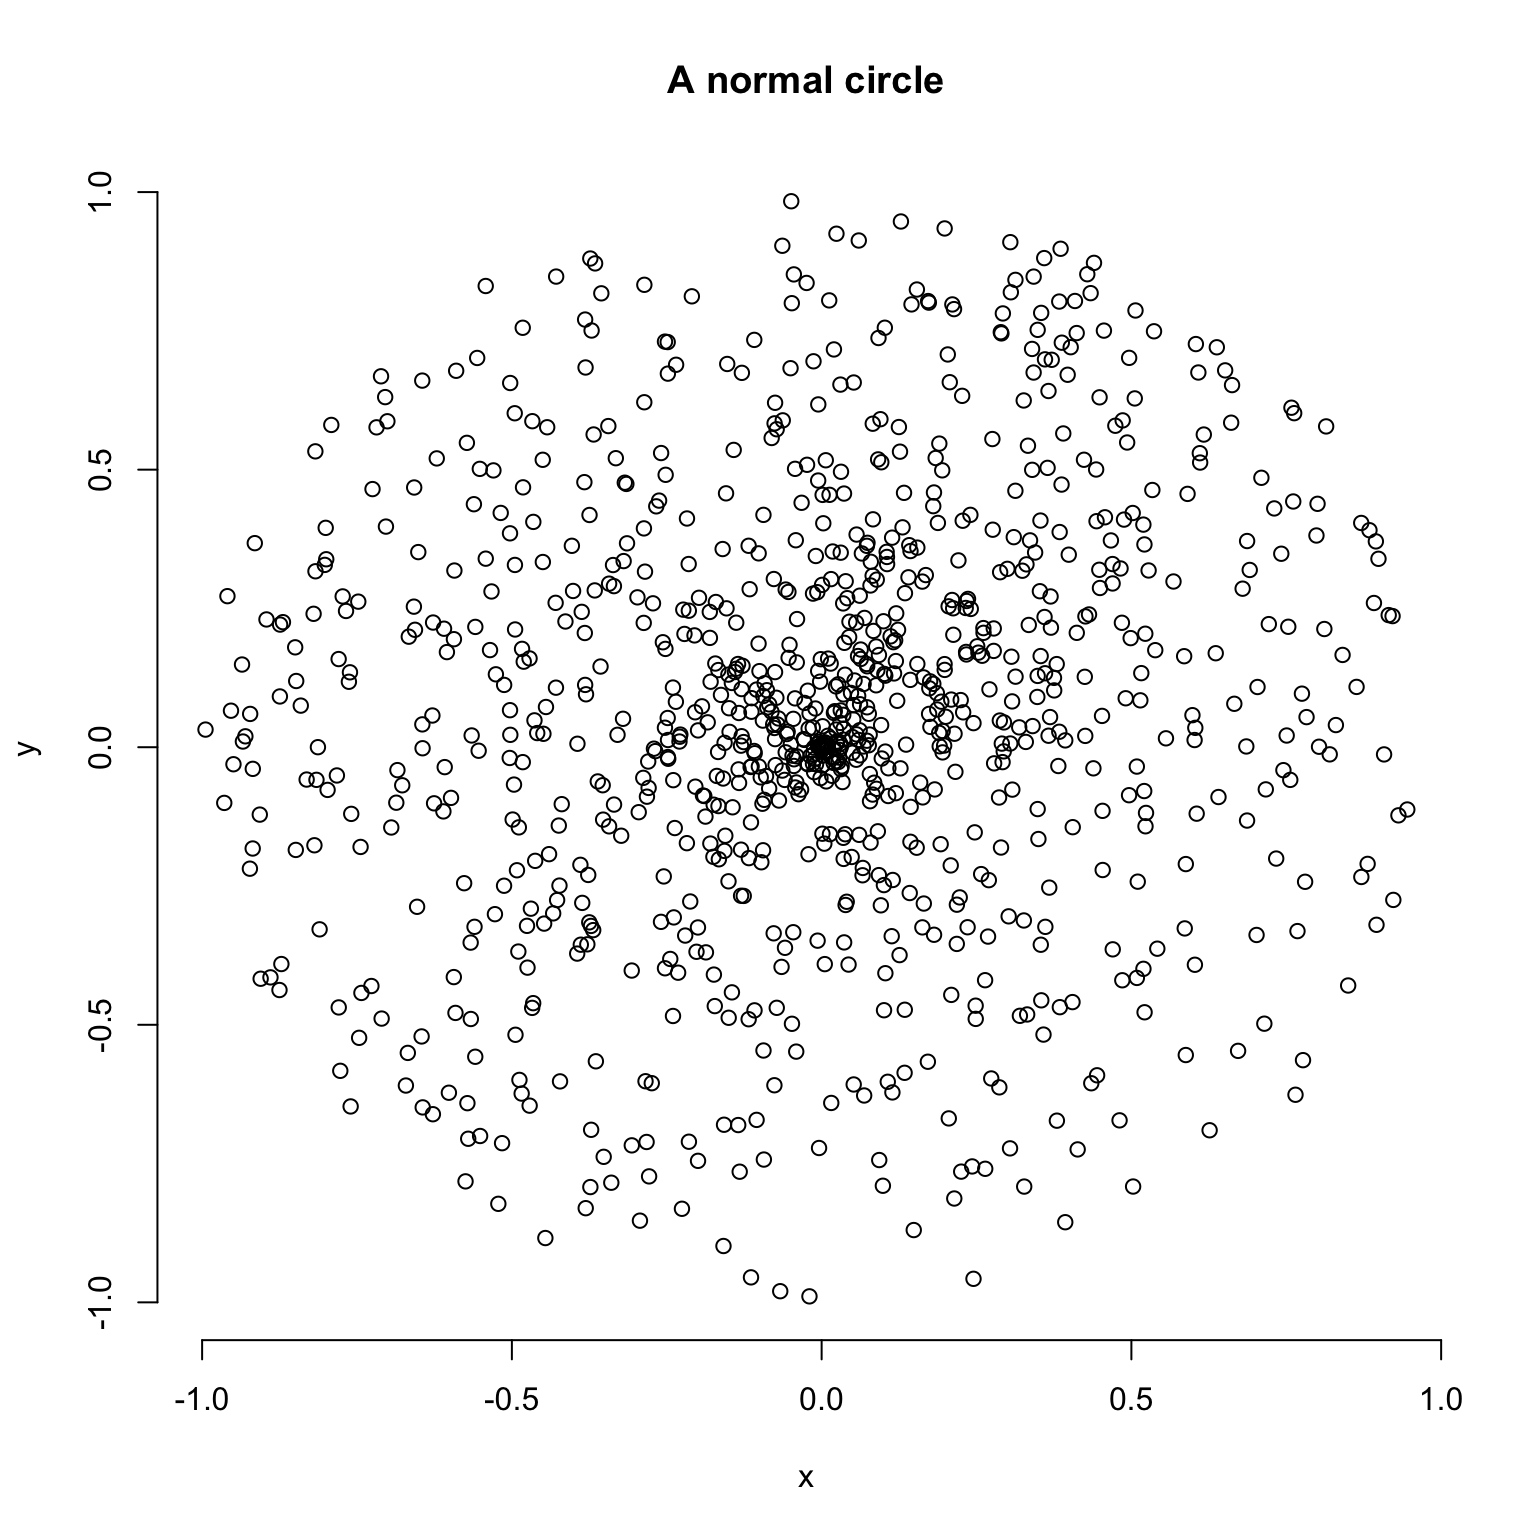
\includegraphics{dispRity_manual_files/figure-latex/unnamed-chunk-79-1.pdf}

\begin{quote}
You can have an even nicer looking tree if you use the \texttt{strap}
package!
\end{quote}

\begin{Shaded}
\begin{Highlighting}[]
\ControlFlowTok{if}\NormalTok{(}\OperatorTok{!}\KeywordTok{require}\NormalTok{(strap)) }\KeywordTok{install.packages}\NormalTok{(}\StringTok{"strap"}\NormalTok{)}
\NormalTok{strap}\OperatorTok{::}\KeywordTok{geoscalePhylo}\NormalTok{(BeckLee_tree, }\DataTypeTok{cex.tip =} \FloatTok{0.7}\NormalTok{, }\DataTypeTok{cex.ts =} \FloatTok{0.6}\NormalTok{)}
\end{Highlighting}
\end{Shaded}

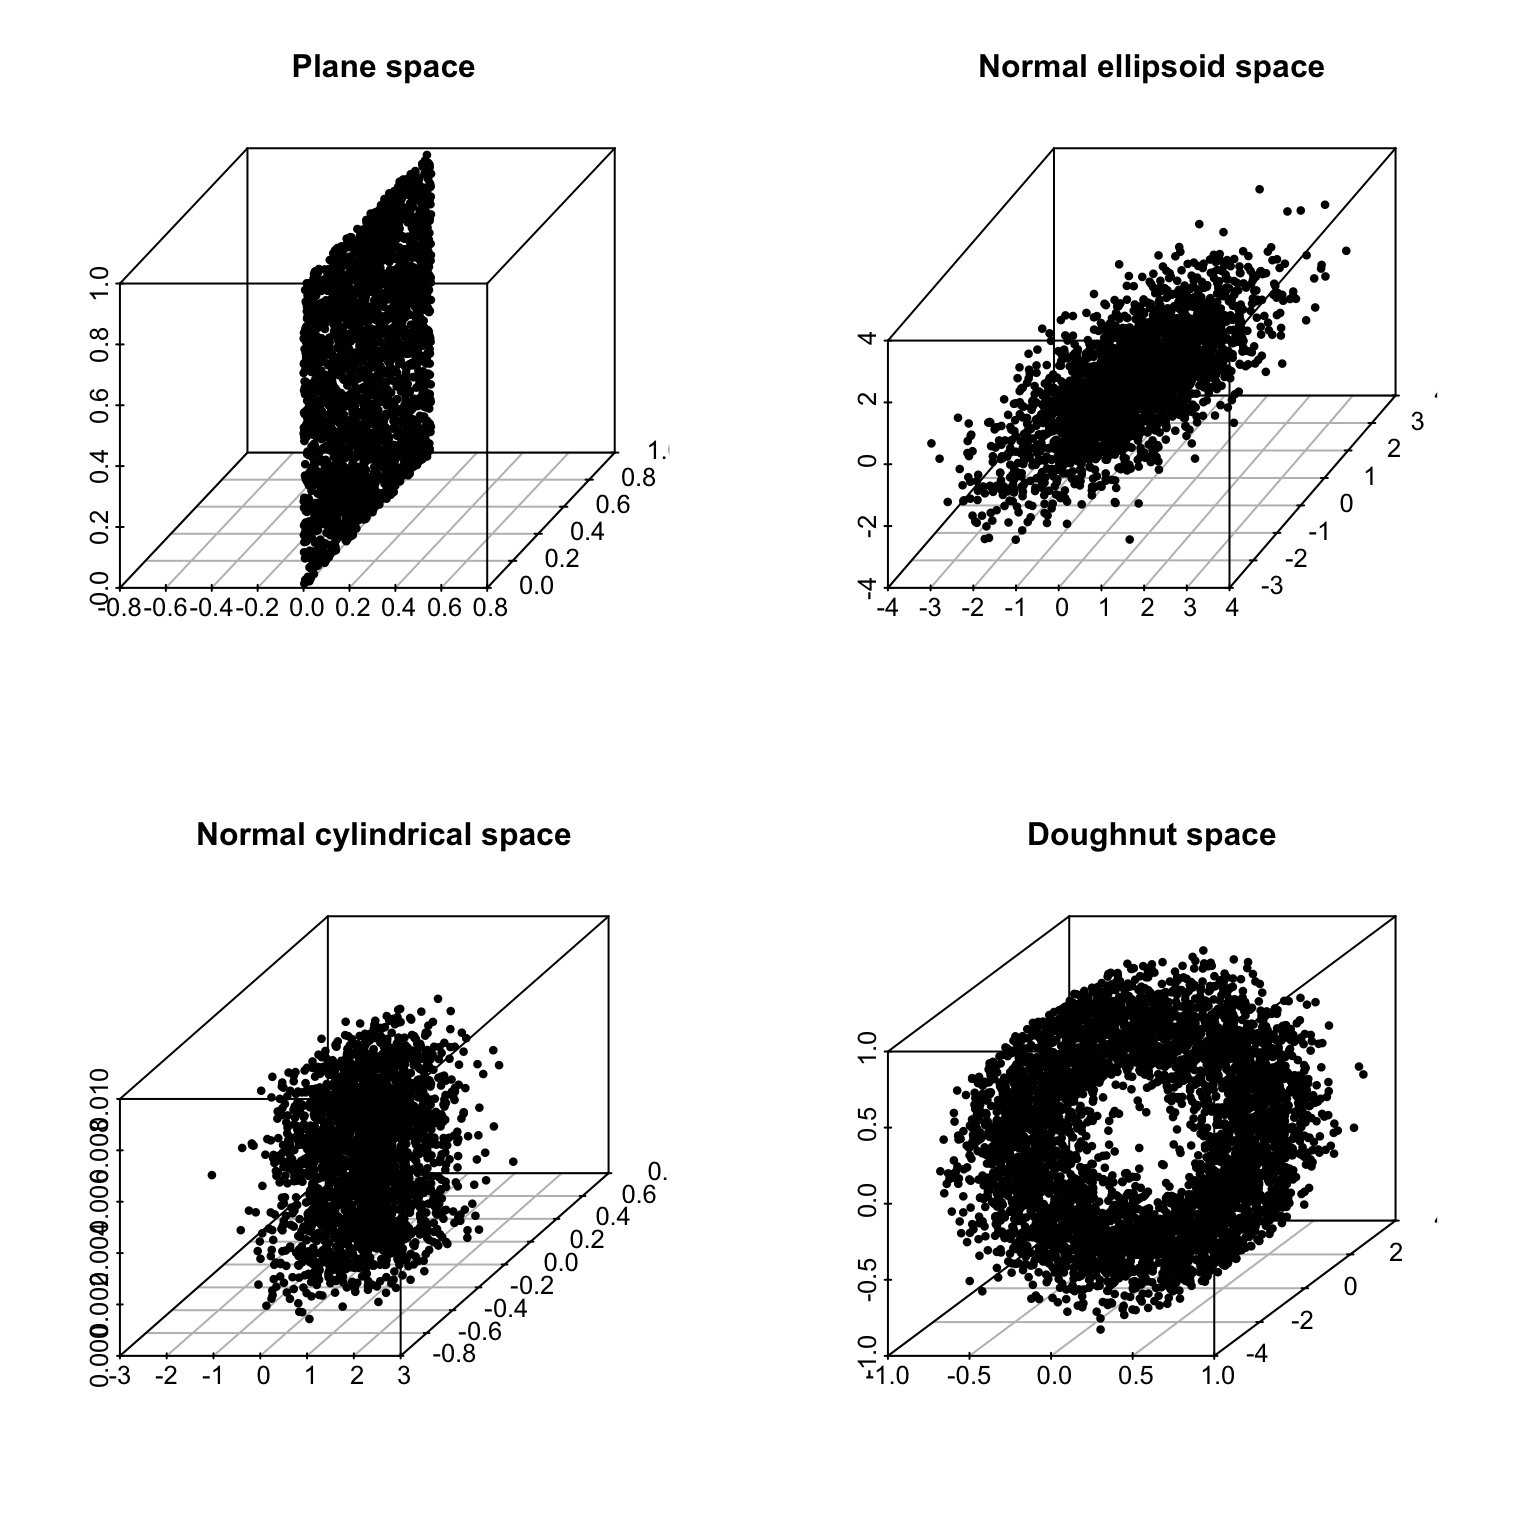
\includegraphics{dispRity_manual_files/figure-latex/unnamed-chunk-80-1.pdf}

\section{A disparity-through-time
analysis}\label{a-disparity-through-time-analysis}

\subsection{Splitting the morphospace through
time}\label{splitting-the-morphospace-through-time}

One of the crucial steps in disparity-through-time analysis is to split
the full morphospace into smaller time subsamples that contain the total
number of morphologies at certain points in time (time-slicing) or
during certain periods in time (time-binning). Basically, the full
morphospace represents the total number of morphologies across all time
and will be greater than any of the time subsamples of the morphospace.

The \texttt{dispRity} package provides a \texttt{time.subsamples}
function that allows users to split the morphospace into time slices
(using \texttt{method\ =\ continuous}) or into time bins (using
\texttt{method\ =\ discrete}). In this example, we are going to split
the morphospace into five equal time bins of 20 million years long from
100 million years ago to the present. We will also provide to the
function a table containing the first and last occurrences dates for
some fossils to take into account that some fossils might occur in
several of our different time bins.

\begin{Shaded}
\begin{Highlighting}[]
\NormalTok{## Creating the vector of time bins ages}
\NormalTok{(time_bins <-}\StringTok{ }\KeywordTok{rev}\NormalTok{(}\KeywordTok{seq}\NormalTok{(}\DataTypeTok{from =} \DecValTok{0}\NormalTok{, }\DataTypeTok{to =} \DecValTok{100}\NormalTok{, }\DataTypeTok{by =} \DecValTok{20}\NormalTok{)))}
\end{Highlighting}
\end{Shaded}

\begin{verbatim}
## [1] 100  80  60  40  20   0
\end{verbatim}

\begin{Shaded}
\begin{Highlighting}[]
\NormalTok{## Splitting the morphospace using the time.subsamples function}
\NormalTok{(binned_morphospace <-}\StringTok{ }\KeywordTok{time.subsamples}\NormalTok{(}\DataTypeTok{data =}\NormalTok{ BeckLee_mat50, }\DataTypeTok{tree =}\NormalTok{ BeckLee_tree,}
    \DataTypeTok{method =} \StringTok{"discrete"}\NormalTok{, }\DataTypeTok{time =}\NormalTok{ time_bins, }\DataTypeTok{inc.nodes =} \OtherTok{FALSE}\NormalTok{,}
    \DataTypeTok{FADLAD =}\NormalTok{ BeckLee_ages))}
\end{Highlighting}
\end{Shaded}

\begin{verbatim}
##  ---- dispRity object ---- 
## 5 discrete time subsamples for 50 elements:
##     100 - 80, 80 - 60, 60 - 40, 40 - 20, 20 - 0.
\end{verbatim}

The output object is a \texttt{dispRity} object (see more about that
\protect\hyperlink{The-guts-of-the-dispRity-package}{here}. In brief,
however, \texttt{dispRity} objects are lists of different elements
(i.e.~disparity results, morphospace time subsamples, morphospace
attributes, etc.) that display only a summary of the object when calling
the object to avoiding filling the \texttt{R} console with superfluous
output.

\begin{Shaded}
\begin{Highlighting}[]
\NormalTok{## Printing the class of the object}
\KeywordTok{class}\NormalTok{(binned_morphospace)}
\end{Highlighting}
\end{Shaded}

\begin{verbatim}
## [1] "dispRity"
\end{verbatim}

\begin{Shaded}
\begin{Highlighting}[]
\NormalTok{## Printing the content of the object}
\KeywordTok{str}\NormalTok{(binned_morphospace)}
\end{Highlighting}
\end{Shaded}

\begin{verbatim}
## List of 3
##  $ matrix    : num [1:50, 1:48] -0.532 -0.409 -0.692 -0.68 -0.739 ...
##   ..- attr(*, "dimnames")=List of 2
##   .. ..$ : chr [1:50] "Cimolestes" "Maelestes" "Batodon" "Bulaklestes" ...
##   .. ..$ : NULL
##  $ call      :List of 1
##   ..$ subsamples: chr "discrete"
##  $ subsamples:List of 5
##   ..$ 100 - 80:List of 1
##   .. ..$ elements: int [1:8, 1] 5 4 6 8 43 10 11 42
##   ..$ 80 - 60 :List of 1
##   .. ..$ elements: int [1:15, 1] 7 8 9 1 2 3 12 13 14 44 ...
##   ..$ 60 - 40 :List of 1
##   .. ..$ elements: int [1:13, 1] 41 49 24 25 26 27 28 21 22 19 ...
##   ..$ 40 - 20 :List of 1
##   .. ..$ elements: int [1:6, 1] 15 39 40 35 23 47
##   ..$ 20 - 0  :List of 1
##   .. ..$ elements: int [1:10, 1] 36 37 38 32 33 34 50 48 29 30
##  - attr(*, "class")= chr "dispRity"
\end{verbatim}

\begin{Shaded}
\begin{Highlighting}[]
\KeywordTok{names}\NormalTok{(binned_morphospace)}
\end{Highlighting}
\end{Shaded}

\begin{verbatim}
## [1] "matrix"     "call"       "subsamples"
\end{verbatim}

\begin{Shaded}
\begin{Highlighting}[]
\NormalTok{## Printing the object as a dispRity class}
\NormalTok{binned_morphospace}
\end{Highlighting}
\end{Shaded}

\begin{verbatim}
##  ---- dispRity object ---- 
## 5 discrete time subsamples for 50 elements:
##     100 - 80, 80 - 60, 60 - 40, 40 - 20, 20 - 0.
\end{verbatim}

\begin{quote}
These objects will gradually contain more information when completing
the following steps in the disparity-through-time analysis.
\end{quote}

\subsection{Bootstrapping the data}\label{bootstrapping-the-data}

Once we obtain our different time subsamples, we can bootstrap and
rarefy them (i.e.~pseudo-replicating the data). The bootstrapping allows
us to make each subsample more robust to outliers and the rarefaction
allows us to compare subsamples with the same number of taxa to remove
sampling biases (i.e.~more taxa in one subsample than the others). The
\texttt{boot.matrix} function bootstraps the \texttt{dispRity} object
and the \texttt{rarefaction} option within performs rarefaction.

\begin{Shaded}
\begin{Highlighting}[]
\NormalTok{## Bootstrapping each time subsample 100 times (default)}
\NormalTok{(boot_bin_morphospace <-}\StringTok{ }\KeywordTok{boot.matrix}\NormalTok{(binned_morphospace))}
\end{Highlighting}
\end{Shaded}

\begin{verbatim}
##  ---- dispRity object ---- 
## 5 discrete time subsamples for 50 elements with 48 dimensions:
##     100 - 80, 80 - 60, 60 - 40, 40 - 20, 20 - 0.
## Data was bootstrapped 100 times (method:"full").
\end{verbatim}

\begin{Shaded}
\begin{Highlighting}[]
\NormalTok{## Getting the minimum number of rows (i.e. taxa) in the time subsamples}
\KeywordTok{min}\NormalTok{(}\KeywordTok{size.subsamples}\NormalTok{(boot_bin_morphospace))}
\end{Highlighting}
\end{Shaded}

\begin{verbatim}
## [1] 6
\end{verbatim}

\begin{Shaded}
\begin{Highlighting}[]
\NormalTok{## Bootstrapping each time subsample 100 times and rarefying them }
\NormalTok{(rare_bin_morphospace <-}\StringTok{ }\KeywordTok{boot.matrix}\NormalTok{(binned_morphospace, }\DataTypeTok{bootstraps =} \DecValTok{100}\NormalTok{,}
    \DataTypeTok{rarefaction =} \DecValTok{6}\NormalTok{))}
\end{Highlighting}
\end{Shaded}

\begin{verbatim}
##  ---- dispRity object ---- 
## 5 discrete time subsamples for 50 elements with 48 dimensions:
##     100 - 80, 80 - 60, 60 - 40, 40 - 20, 20 - 0.
## Data was bootstrapped 100 times (method:"full") and rarefied to 6 elements.
\end{verbatim}

\subsection{Calculating disparity}\label{calculating-disparity}

We can now calculate the disparity within each time subsamples along
with some confidence intervals generated by the pseudoreplication step
above (bootstraps/rarefaction). Disparity can be calculated in many ways
and this package allows users to come up with their own disparity
metrics. For more details, please refer to the
\protect\hyperlink{disparity-metrics}{\texttt{dispRity} metric section}.

In this example, we are going to calculate the spread of the data in
each time subsample by calculating disparity as the sum of the variance
of each dimension of the morphospace in each time subsample using the
\texttt{dispRity} function. Thus, in this example, disparity is defined
by the multi-dimensional variance of each time subsample (i.e.~the
spread of the taxa within the morphospace). Note that this metric comes
with a caveat (not solved here) since it ignores covariances among the
dimensions of the morphospace. We use this here because it is a standard
metric used in disparity-through-time analysis (Wills \emph{et al.}
1994).

\begin{Shaded}
\begin{Highlighting}[]
\NormalTok{## Calculating disparity for the bootstrapped data}
\NormalTok{(boot_disparity <-}\StringTok{ }\KeywordTok{dispRity}\NormalTok{(boot_bin_morphospace, }\DataTypeTok{metric =} \KeywordTok{c}\NormalTok{(sum, variances)))}
\end{Highlighting}
\end{Shaded}

\begin{verbatim}
##  ---- dispRity object ---- 
## 5 discrete time subsamples for 50 elements with 48 dimensions:
##     100 - 80, 80 - 60, 60 - 40, 40 - 20, 20 - 0.
## Data was bootstrapped 100 times (method:"full").
## Disparity was calculated as: c(sum, variances).
\end{verbatim}

\begin{Shaded}
\begin{Highlighting}[]
\NormalTok{## Calculating disparity for the rarefied data}
\NormalTok{(rare_disparity <-}\StringTok{ }\KeywordTok{dispRity}\NormalTok{(rare_bin_morphospace, }\DataTypeTok{metric =} \KeywordTok{c}\NormalTok{(sum, variances)))}
\end{Highlighting}
\end{Shaded}

\begin{verbatim}
##  ---- dispRity object ---- 
## 5 discrete time subsamples for 50 elements with 48 dimensions:
##     100 - 80, 80 - 60, 60 - 40, 40 - 20, 20 - 0.
## Data was bootstrapped 100 times (method:"full") and rarefied to 6 elements.
## Disparity was calculated as: c(sum, variances).
\end{verbatim}

The \texttt{dispRity} function does not actually display the calculated
disparity values but rather only the properties of the disparity object
(size, subsamples, metric, etc.). To display the actual calculated
scores, we need to summarise the disparity object using the S3 method
\texttt{summary} that is applied to a \texttt{dispRity} object (see
\texttt{?summary.dispRity} for more details).

As for any \texttt{R} package, you can refer to the help files for each
individual function for more details.

\begin{Shaded}
\begin{Highlighting}[]
\NormalTok{## Summarising the disparity results}
\KeywordTok{summary}\NormalTok{(boot_disparity)}
\end{Highlighting}
\end{Shaded}

\begin{verbatim}
##   subsamples  n   obs bs.median  2.5%   25%   75% 97.5%
## 1   100 - 80  8 1.675     1.488 1.087 1.389 1.568 1.648
## 2    80 - 60 15 1.782     1.679 1.538 1.631 1.728 1.792
## 3    60 - 40 13 1.913     1.772 1.607 1.734 1.826 1.886
## 4    40 - 20  6 2.022     1.707 1.212 1.537 1.822 1.942
## 5     20 - 0 10 1.971     1.794 1.598 1.716 1.842 1.890
\end{verbatim}

\begin{Shaded}
\begin{Highlighting}[]
\KeywordTok{summary}\NormalTok{(rare_disparity)}
\end{Highlighting}
\end{Shaded}

\begin{verbatim}
##   subsamples  n   obs bs.median  2.5%   25%   75% 97.5%
## 1   100 - 80  8 1.675     1.484 1.194 1.400 1.547 1.636
## 2   100 - 80  6    NA     1.477 0.993 1.361 1.569 1.698
## 3    80 - 60 15 1.782     1.674 1.517 1.600 1.725 1.793
## 4    80 - 60  6    NA     1.655 1.299 1.532 1.754 1.882
## 5    60 - 40 13 1.913     1.767 1.601 1.714 1.829 1.861
## 6    60 - 40  6    NA     1.787 1.314 1.672 1.879 1.984
## 7    40 - 20  6 2.022     1.736 1.281 1.603 1.822 1.948
## 8     20 - 0 10 1.971     1.807 1.595 1.729 1.856 1.917
## 9     20 - 0  6    NA     1.790 1.435 1.718 1.873 1.995
\end{verbatim}

\begin{quote}
The summary.dispRity function comes with many options on which values to
calculate (central tendency and quantiles) and on how many digits to
display. Refer to the function's manual for more details.
\end{quote}

\subsection{Plotting the results}\label{plotting-the-results}

It is sometimes easier to visualise the results in a plot than in a
table. For that we can use the \texttt{plot} S3 function to plot the
\texttt{dispRity} objects (see \texttt{?plot.dispRity} for more
details).

\begin{Shaded}
\begin{Highlighting}[]
\NormalTok{## Graphical options}
\KeywordTok{quartz}\NormalTok{(}\DataTypeTok{width =} \DecValTok{10}\NormalTok{, }\DataTypeTok{height =} \DecValTok{5}\NormalTok{) ; }\KeywordTok{par}\NormalTok{(}\DataTypeTok{mfrow =}\NormalTok{ (}\KeywordTok{c}\NormalTok{(}\DecValTok{1}\NormalTok{,}\DecValTok{2}\NormalTok{)), }\DataTypeTok{bty =} \StringTok{"n"}\NormalTok{)}

\NormalTok{## Plotting the bootstrapped and rarefied results}
\KeywordTok{plot}\NormalTok{(boot_disparity, }\DataTypeTok{type =} \StringTok{"continuous"}\NormalTok{, }\DataTypeTok{main =} \StringTok{"bootstrapped results"}\NormalTok{)}
\KeywordTok{plot}\NormalTok{(rare_disparity, }\DataTypeTok{type =} \StringTok{"continuous"}\NormalTok{, }\DataTypeTok{main =} \StringTok{"rarefied results"}\NormalTok{)}
\end{Highlighting}
\end{Shaded}

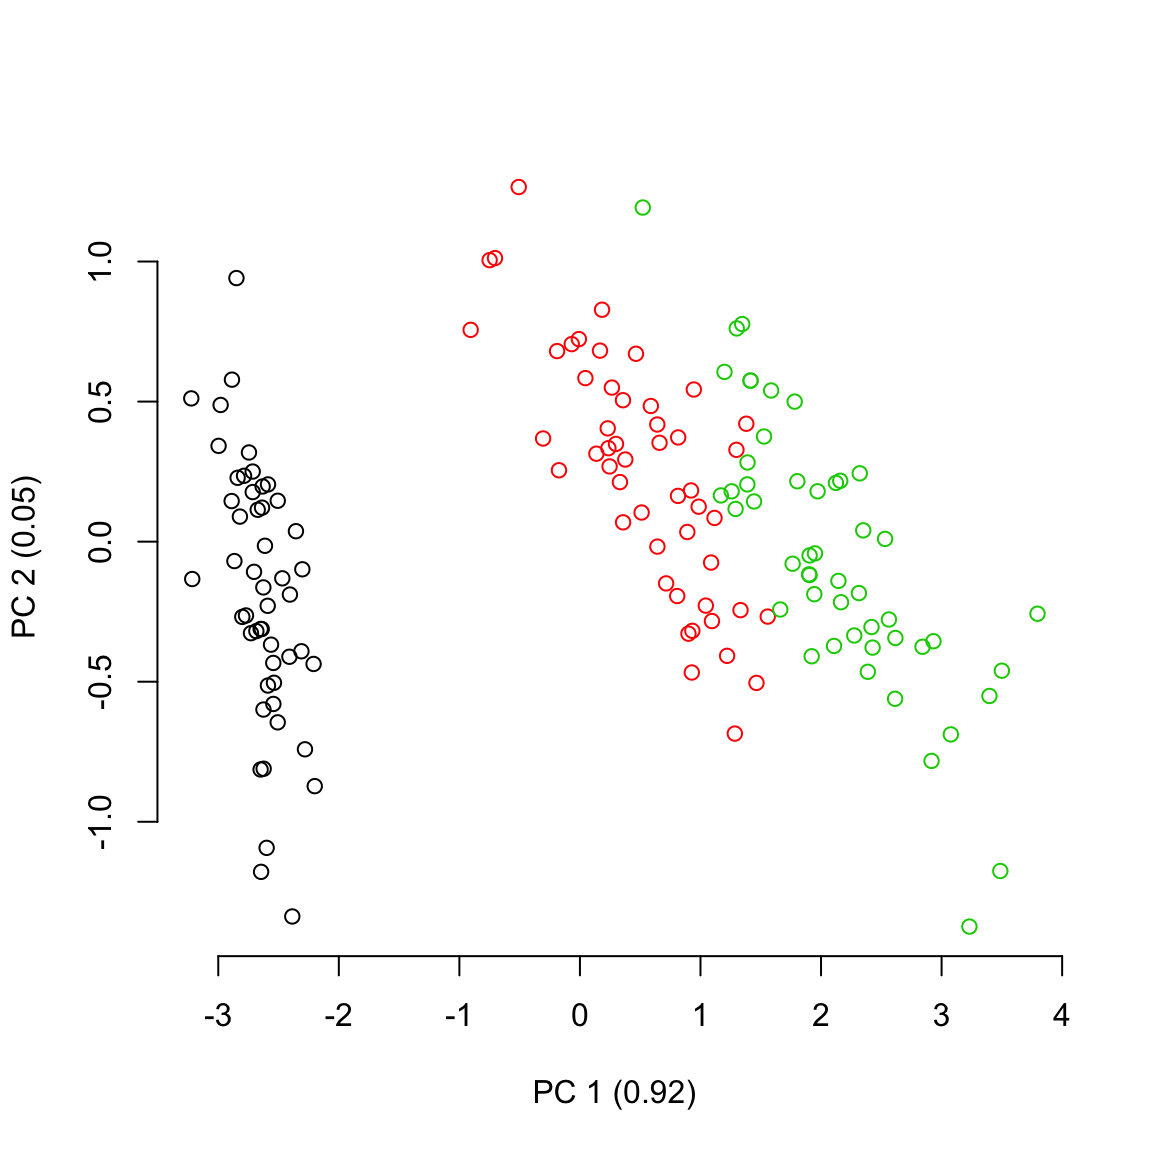
\includegraphics{dispRity_manual_files/figure-latex/unnamed-chunk-86-1.pdf}

\section{Testing differences}\label{testing-differences}

Finally, to draw some valid conclusions from these results, we can apply
some statistical tests. We can test, for example, if mammalian disparity
changed significantly through time over the last 100 million years. To
do so, we can compare the means of each time-bin in a sequential manner
to see whether the disparity in bin \emph{n} is equal to the disparity
in bin \emph{n+1}, and whether this is in turn equal to the disparity in
bin \emph{n+2}, etc. Because our data is temporally autocorrelated
(i.e.~what happens in bin \emph{n+1} depends on what happened in bin
\emph{n}) and pseudoreplicated (i.e.~each bootstrap draw creates
non-independent time subsamples because they are all based on the same
time subsamples), we apply a non-parametric mean comparison: the
\texttt{wilcox.test}. Also, we need to apply a p-value correction
(e.g.~Bonferroni correction) to correct for multiple testing (see
\texttt{?p.adjust} for more details).

\begin{Shaded}
\begin{Highlighting}[]
\NormalTok{## Testing the differences between bins in the bootstrapped dataset.}
\KeywordTok{test.dispRity}\NormalTok{(boot_disparity, }\DataTypeTok{test =}\NormalTok{ wilcox.test, }\DataTypeTok{comparison =} \StringTok{"sequential"}\NormalTok{,}
    \DataTypeTok{correction =} \StringTok{"bonferroni"}\NormalTok{)}
\end{Highlighting}
\end{Shaded}

\begin{verbatim}
## [[1]]
##                    statistic
## 100 - 80 : 80 - 60       471
## 80 - 60 : 60 - 40       1562
## 60 - 40 : 40 - 20       6250
## 40 - 20 : 20 - 0        3725
## 
## [[2]]
##                         p.value
## 100 - 80 : 80 - 60 7.427563e-28
## 80 - 60 : 60 - 40  1.798899e-16
## 60 - 40 : 40 - 20  9.061511e-03
## 40 - 20 : 20 - 0   7.379715e-03
\end{verbatim}

\begin{Shaded}
\begin{Highlighting}[]
\NormalTok{## Testing the differences between bins in the rarefied dataset.}
\KeywordTok{test.dispRity}\NormalTok{(rare_disparity, }\DataTypeTok{test =}\NormalTok{ wilcox.test, }\DataTypeTok{comparison =} \StringTok{"sequential"}\NormalTok{,}
    \DataTypeTok{correction =} \StringTok{"bonferroni"}\NormalTok{)}
\end{Highlighting}
\end{Shaded}

\begin{verbatim}
## [[1]]
##                    statistic
## 100 - 80 : 80 - 60       662
## 80 - 60 : 60 - 40       1814
## 60 - 40 : 40 - 20       5752
## 40 - 20 : 20 - 0        3621
## 
## [[2]]
##                         p.value
## 100 - 80 : 80 - 60 1.214988e-25
## 80 - 60 : 60 - 40  2.823697e-14
## 60 - 40 : 40 - 20  2.653018e-01
## 40 - 20 : 20 - 0   3.026079e-03
\end{verbatim}

Here our results show significant changes in disparity through time
between all time bins (all p-values \textless{} 0.05). However, when
looking at the rarefied results, there is no significant difference
between the time bins in the Palaeogene (60-40 to 40-20 Mya), suggesting
that the differences detected in the first test might just be due to the
differences in number of taxa sampled (13 or 6 taxa) in each time bin.

\chapter{Ecology demo}\label{ecology-demo}

This is an example of typical disparity analysis that can be performed
in ecology.

\section{Data}\label{data}

For this example, we will use the famous \texttt{iris} inbuilt data set

\begin{Shaded}
\begin{Highlighting}[]
\KeywordTok{data}\NormalTok{(iris)}
\end{Highlighting}
\end{Shaded}

This data contains petal and sepal length for 150 individual plants
sorted into three species.

\begin{Shaded}
\begin{Highlighting}[]
\NormalTok{## Separating the species}
\NormalTok{species <-}\StringTok{ }\NormalTok{iris[,}\DecValTok{5}\NormalTok{]}
\NormalTok{## Which species?}
\KeywordTok{unique}\NormalTok{(species)}
\end{Highlighting}
\end{Shaded}

\begin{verbatim}
## [1] setosa     versicolor virginica 
## Levels: setosa versicolor virginica
\end{verbatim}

\begin{Shaded}
\begin{Highlighting}[]
\NormalTok{## Separating the petal/sepal length}
\NormalTok{measurements <-}\StringTok{ }\NormalTok{iris[,}\DecValTok{1}\OperatorTok{:}\DecValTok{4}\NormalTok{]}
\KeywordTok{head}\NormalTok{(measurements)}
\end{Highlighting}
\end{Shaded}

\begin{verbatim}
##   Sepal.Length Sepal.Width Petal.Length Petal.Width
## 1          5.1         3.5          1.4         0.2
## 2          4.9         3.0          1.4         0.2
## 3          4.7         3.2          1.3         0.2
## 4          4.6         3.1          1.5         0.2
## 5          5.0         3.6          1.4         0.2
## 6          5.4         3.9          1.7         0.4
\end{verbatim}

We can then ordinate the data using a PCA (\texttt{prcomp} function)
thus defining our four dimensional space as the poetically named
petal-space.

\begin{Shaded}
\begin{Highlighting}[]
\NormalTok{## Ordinating the data}
\NormalTok{ordination <-}\StringTok{ }\KeywordTok{prcomp}\NormalTok{(measurements)}

\NormalTok{## The petal-space}
\NormalTok{petal_space <-}\StringTok{ }\NormalTok{ordination}\OperatorTok{$}\NormalTok{x}

\NormalTok{## Adding the elements names to the petal-space (the individuals IDs)}
\KeywordTok{rownames}\NormalTok{(petal_space) <-}\StringTok{ }\DecValTok{1}\OperatorTok{:}\KeywordTok{nrow}\NormalTok{(petal_space)}
\end{Highlighting}
\end{Shaded}

\section{Classic analysis}\label{classic-analysis}

A classical way to represent this ordinated data would be to use two
dimensional plots to look at how the different species are distributed
in the petal-space.

\begin{Shaded}
\begin{Highlighting}[]
\NormalTok{## Measuring the variance on each axis}
\NormalTok{variances <-}\StringTok{ }\KeywordTok{apply}\NormalTok{(petal_space, }\DecValTok{2}\NormalTok{, var)}
\NormalTok{variances <-}\StringTok{ }\NormalTok{variances}\OperatorTok{/}\KeywordTok{sum}\NormalTok{(variances)}

\NormalTok{## Graphical option}
\KeywordTok{par}\NormalTok{(}\DataTypeTok{bty =} \StringTok{"n"}\NormalTok{)}

\NormalTok{## A classic 2D ordination plot}
\KeywordTok{plot}\NormalTok{(petal_space[, }\DecValTok{1}\NormalTok{], petal_space[, }\DecValTok{2}\NormalTok{], }\DataTypeTok{col =}\NormalTok{ species,}
    \DataTypeTok{xlab =} \KeywordTok{paste0}\NormalTok{(}\StringTok{"PC 1 ("}\NormalTok{, }\KeywordTok{round}\NormalTok{(variances[}\DecValTok{1}\NormalTok{], }\DecValTok{2}\NormalTok{), }\StringTok{")"}\NormalTok{),}
    \DataTypeTok{ylab =} \KeywordTok{paste0}\NormalTok{(}\StringTok{"PC 2 ("}\NormalTok{, }\KeywordTok{round}\NormalTok{(variances[}\DecValTok{2}\NormalTok{], }\DecValTok{2}\NormalTok{), }\StringTok{")"}\NormalTok{))}
\end{Highlighting}
\end{Shaded}

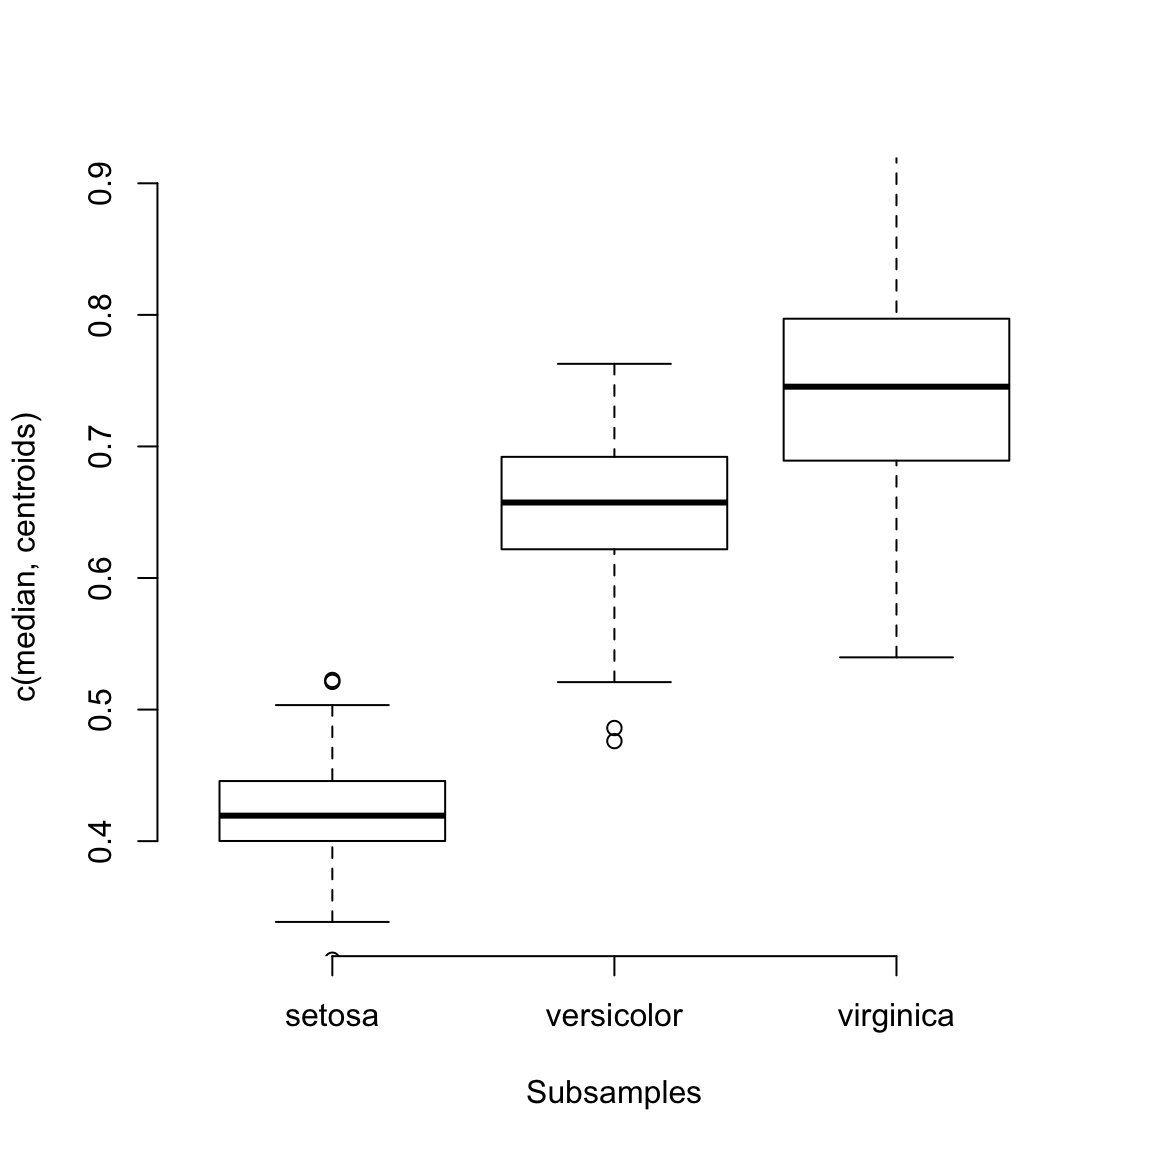
\includegraphics{dispRity_manual_files/figure-latex/unnamed-chunk-91-1.pdf}

This shows the distribution of the different species in the petal-space
along the two first axis of variation. This is a pretty standard way to
visualise the multidimensional space and further analysis might be
necessary to test wether the groups are different such as a linear
discriminant analysis (LDA). However, in this case we are ignoring the
two other dimensions of the ordination! If we look at the two other axis
we see a totally different result:

\begin{Shaded}
\begin{Highlighting}[]
\NormalTok{## Plotting the two second axis of the petal-space}
\KeywordTok{plot}\NormalTok{(petal_space[, }\DecValTok{3}\NormalTok{], petal_space[, }\DecValTok{4}\NormalTok{], }\DataTypeTok{col =}\NormalTok{ species,}
    \DataTypeTok{xlab =} \KeywordTok{paste0}\NormalTok{(}\StringTok{"PC 3 ("}\NormalTok{, }\KeywordTok{round}\NormalTok{(variances[}\DecValTok{3}\NormalTok{], }\DecValTok{2}\NormalTok{), }\StringTok{")"}\NormalTok{),}
    \DataTypeTok{ylab =} \KeywordTok{paste0}\NormalTok{(}\StringTok{"PC 4 ("}\NormalTok{, }\KeywordTok{round}\NormalTok{(variances[}\DecValTok{4}\NormalTok{], }\DecValTok{2}\NormalTok{), }\StringTok{")"}\NormalTok{))}
\end{Highlighting}
\end{Shaded}

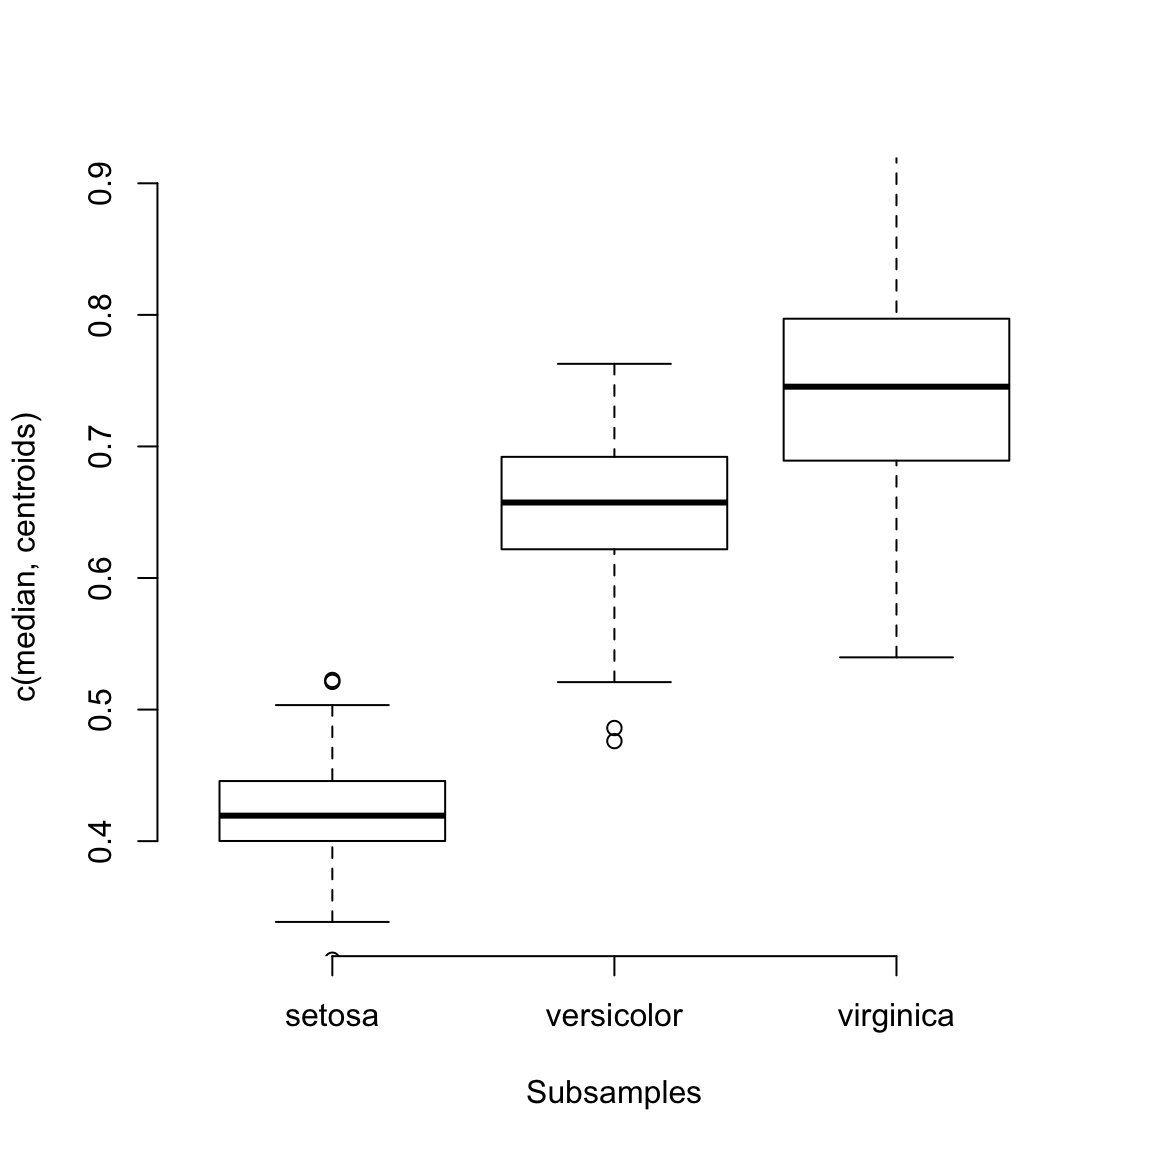
\includegraphics{dispRity_manual_files/figure-latex/unnamed-chunk-92-1.pdf}

Additionally, these two represented dimensions do not represent a
biological reality \emph{per se}; i.e.~the values on the first dimension
do not represent a continuous trait (e.g.~petal length), instead they
just represent the ordinations of correlations between the data and some
factors.

Therefore, we might want to approach this problem without getting stuck
in only two dimensions and consider the whole dataset as a
\emph{n}-dimensional object.

\section{\texorpdfstring{A multidimensional approach with
\texttt{dispRity}}{A multidimensional approach with dispRity}}\label{a-multidimensional-approach-with-disprity}

The first step is to create different subsamples that represent
subsamples of the ordinated space (i.e.~sub-regions within the
\emph{n}-dimensional object). Each of these subsamples will contain only
the individuals of a specific species.

\begin{Shaded}
\begin{Highlighting}[]
\NormalTok{## Creating the table that contain the elements and their attributes}
\NormalTok{petal_subsamples <-}\StringTok{ }\KeywordTok{custom.subsamples}\NormalTok{(petal_space, }\DataTypeTok{group =} \KeywordTok{list}\NormalTok{(}
                                \StringTok{"setosa"}\NormalTok{ =}\StringTok{ }\KeywordTok{which}\NormalTok{(species }\OperatorTok{==}\StringTok{ "setosa"}\NormalTok{),}
                                \StringTok{"versicolor"}\NormalTok{ =}\StringTok{ }\KeywordTok{which}\NormalTok{(species }\OperatorTok{==}\StringTok{ "versicolor"}\NormalTok{),}
                                \StringTok{"virginica"}\NormalTok{ =}\StringTok{ }\KeywordTok{which}\NormalTok{(species }\OperatorTok{==}\StringTok{ "virginica"}\NormalTok{)))}

\NormalTok{## Visualising the dispRity object content}
\NormalTok{petal_subsamples}
\end{Highlighting}
\end{Shaded}

\begin{verbatim}
##  ---- dispRity object ---- 
## 3 customised subsamples for 150 elements:
##     setosa, versicolor, virginica.
\end{verbatim}

This created a \texttt{dispRity} object (more about that
\protect\hyperlink{guts}{here}) with three subsamples corresponding to
each subspecies.

\subsection{Bootstrapping the data}\label{bootstrapping-the-data-1}

We can the bootstrap the subsamples to be able test the robustness of
the measured disparity to outliers. We can do that using the default
options of \texttt{boot.matrix} (more about that
\protect\hyperlink{bootstraps-and-rarefactions}{here}):

\begin{Shaded}
\begin{Highlighting}[]
\NormalTok{## Bootstrapping the data}
\NormalTok{(petal_bootstrapped <-}\StringTok{ }\KeywordTok{boot.matrix}\NormalTok{(petal_subsamples))}
\end{Highlighting}
\end{Shaded}

\begin{verbatim}
##  ---- dispRity object ---- 
## 3 customised subsamples for 150 elements with 4 dimensions:
##     setosa, versicolor, virginica.
## Data was bootstrapped 100 times (method:"full").
\end{verbatim}

\subsection{Calculating disparity}\label{calculating-disparity-1}

Disparity can be calculated in many ways, therefore the
\texttt{dispRity} function allows users to define their own measure of
disparity. For more details on measuring disparity, see the
\protect\hyperlink{disparity-metrics}{dispRity metrics section}.

In this example, we are going to define disparity as the median distance
between the different individuals and the centroid of the ordinated
space. High values of disparity will indicate a generally high spread of
points from this centroid (i.e.~on average, the individuals are far
apart in the ordinated space). We can define the metrics easily in the
\texttt{dispRity} function by feeding them to the \texttt{metric}
argument. Here we are going to feed the functions \texttt{stats::median}
and \texttt{dispRity::centroids} which calculates distances between
elements and their centroid.

\begin{Shaded}
\begin{Highlighting}[]
\NormalTok{## Calculating disparity as the median distance between each elements and}
\NormalTok{## the centroid of the petal-space}
\NormalTok{(petal_disparity <-}\StringTok{ }\KeywordTok{dispRity}\NormalTok{(petal_bootstrapped, }\DataTypeTok{metric =} \KeywordTok{c}\NormalTok{(median, centroids)))}
\end{Highlighting}
\end{Shaded}

\begin{verbatim}
##  ---- dispRity object ---- 
## 3 customised subsamples for 150 elements with 4 dimensions:
##     setosa, versicolor, virginica.
## Data was bootstrapped 100 times (method:"full").
## Disparity was calculated as: c(median, centroids).
\end{verbatim}

\subsection{Summarising the results
(plot)}\label{summarising-the-results-plot}

Similarly to the \texttt{custom.subsamples} and \texttt{boot.matrix}
function, \texttt{dispRity} displays a \texttt{dispRity} object. But we
are definitely more interested in actually look at the calculated
values.

First we can summarise the data in a table by simply using
\texttt{summary}:

\begin{Shaded}
\begin{Highlighting}[]
\NormalTok{## Displaying the summary of the calculated disparity}
\KeywordTok{summary}\NormalTok{(petal_disparity)}
\end{Highlighting}
\end{Shaded}

\begin{verbatim}
##   subsamples  n   obs bs.median  2.5%   25%   75% 97.5%
## 1     setosa 50 0.421     0.419 0.342 0.401 0.445 0.503
## 2 versicolor 50 0.693     0.657 0.530 0.622 0.692 0.733
## 3  virginica 50 0.785     0.745 0.577 0.690 0.797 0.880
\end{verbatim}

We can also plot the results in a similar way:

\begin{Shaded}
\begin{Highlighting}[]
\NormalTok{## Graphical options}
\KeywordTok{par}\NormalTok{(}\DataTypeTok{bty =} \StringTok{"n"}\NormalTok{)}

\NormalTok{## Plotting the disparity in the petal_space}
\KeywordTok{plot}\NormalTok{(petal_disparity)}
\end{Highlighting}
\end{Shaded}

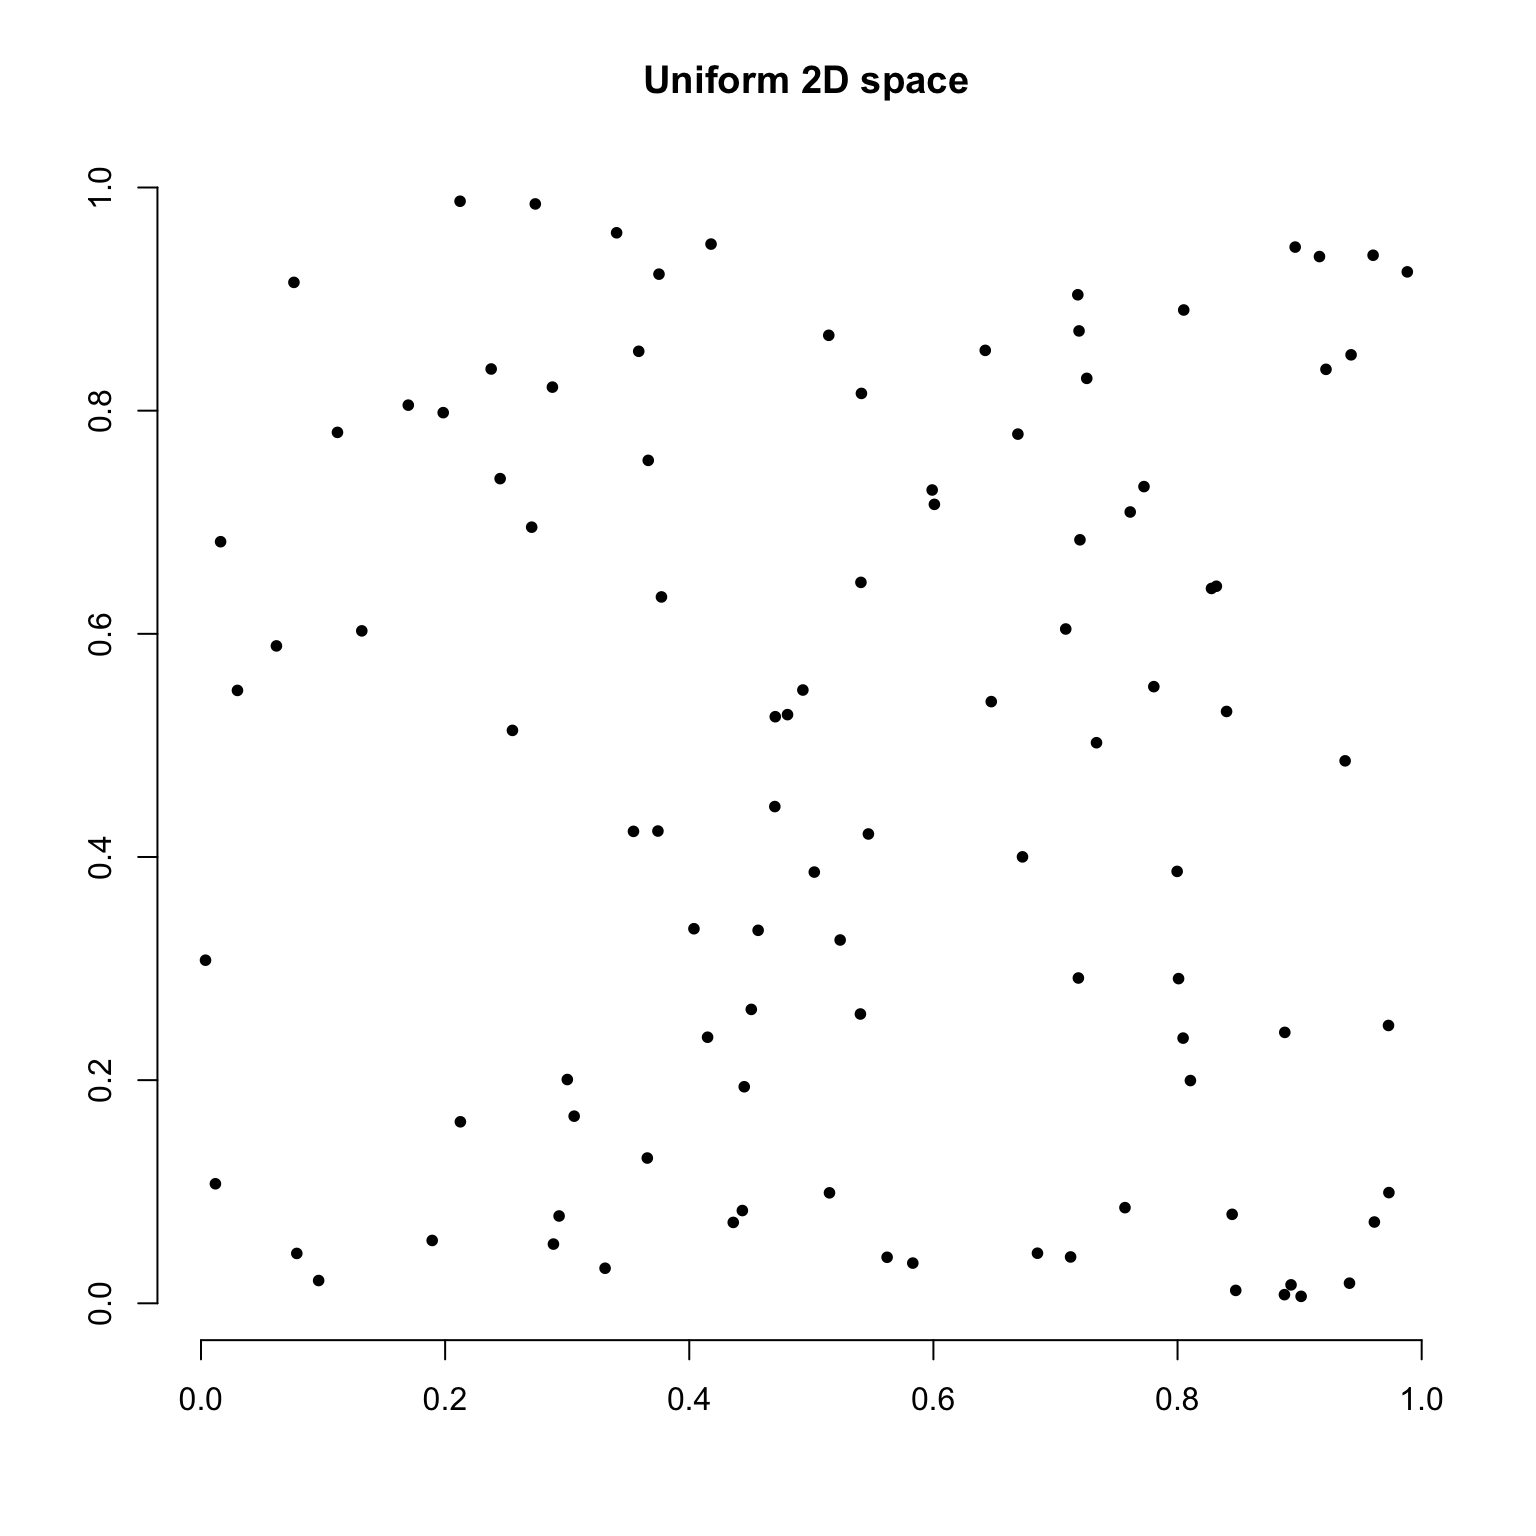
\includegraphics{dispRity_manual_files/figure-latex/unnamed-chunk-97-1.pdf}

Now contrary to simply plotting the two first axis of the PCA where we
saw that the species have a different position in the two first
petal-space, we can now also see that they occupy this space clearly
differently!

\subsection{Testing hypothesis}\label{testing-hypothesis}

Finally we can test our hypothesis that we guessed from the disparity
plot (that some groups occupy different volume of the petal-space) by
using the \texttt{test.dispRity} option.

\begin{Shaded}
\begin{Highlighting}[]
\NormalTok{## Fitting a linear model to our data}
\NormalTok{disparity_lm <-}\StringTok{ }\KeywordTok{test.dispRity}\NormalTok{(petal_disparity, }\DataTypeTok{test =}\NormalTok{ lm, }\DataTypeTok{comparisons =} \StringTok{"all"}\NormalTok{)}
\end{Highlighting}
\end{Shaded}

\begin{verbatim}
## Warning in test.dispRity(petal_disparity, test = lm, comparisons = "all"): Multiple p-values will be calculated without adjustment!
## This will inflate Type I error!
\end{verbatim}

\begin{Shaded}
\begin{Highlighting}[]
\NormalTok{## Testing whether there is a difference in disparity between the different species}
\KeywordTok{summary}\NormalTok{(}\KeywordTok{aov}\NormalTok{(disparity_lm))}
\end{Highlighting}
\end{Shaded}

\begin{verbatim}
##              Df Sum Sq Mean Sq F value Pr(>F)    
## subsamples    2  5.387  2.6935   705.5 <2e-16 ***
## Residuals   297  1.134  0.0038                   
## ---
## Signif. codes:  0 '***' 0.001 '**' 0.01 '*' 0.05 '.' 0.1 ' ' 1
\end{verbatim}

\begin{Shaded}
\begin{Highlighting}[]
\NormalTok{## Post-hoc testing of the differences between species (corrected for multiple tests)}
\KeywordTok{test.dispRity}\NormalTok{(petal_disparity, }\DataTypeTok{test =}\NormalTok{ t.test, }\DataTypeTok{correction =} \StringTok{"bonferroni"}\NormalTok{)}
\end{Highlighting}
\end{Shaded}

\begin{verbatim}
## [[1]]
##                         statistic
## setosa : versicolor    -33.714480
## setosa : virginica     -34.257797
## versicolor : virginica  -8.595829
## 
## [[2]]
##                        parameter
## setosa : versicolor     189.0217
## setosa : virginica      150.1371
## versicolor : virginica  171.2387
## 
## [[3]]
##                             p.value
## setosa : versicolor    2.107278e-81
## setosa : virginica     2.252270e-72
## versicolor : virginica 1.506037e-14
\end{verbatim}

We can now see that there is a significant difference in petal-space
occupancy between all species of iris.

\subsubsection{Setting up a multidimensional
null-hypothesis}\label{setting-up-a-multidimensional-null-hypothesis}

One other series of test can be done on the shape of the petal-space.
Using a MCMC permutation test we can simulate a petal-space with
specific properties and see if our observed petal-space matches these
properties (similarly to Diaz \emph{et al.} 2016):

\begin{Shaded}
\begin{Highlighting}[]
\NormalTok{## Testing against a uniform distribution}
\NormalTok{disparity_uniform <-}\StringTok{ }\KeywordTok{null.test}\NormalTok{(petal_disparity, }\DataTypeTok{replicates =} \DecValTok{200}\NormalTok{,}
    \DataTypeTok{null.distrib =}\NormalTok{ runif, }\DataTypeTok{scale =} \OtherTok{FALSE}\NormalTok{)}
\KeywordTok{plot}\NormalTok{(disparity_uniform)}
\end{Highlighting}
\end{Shaded}

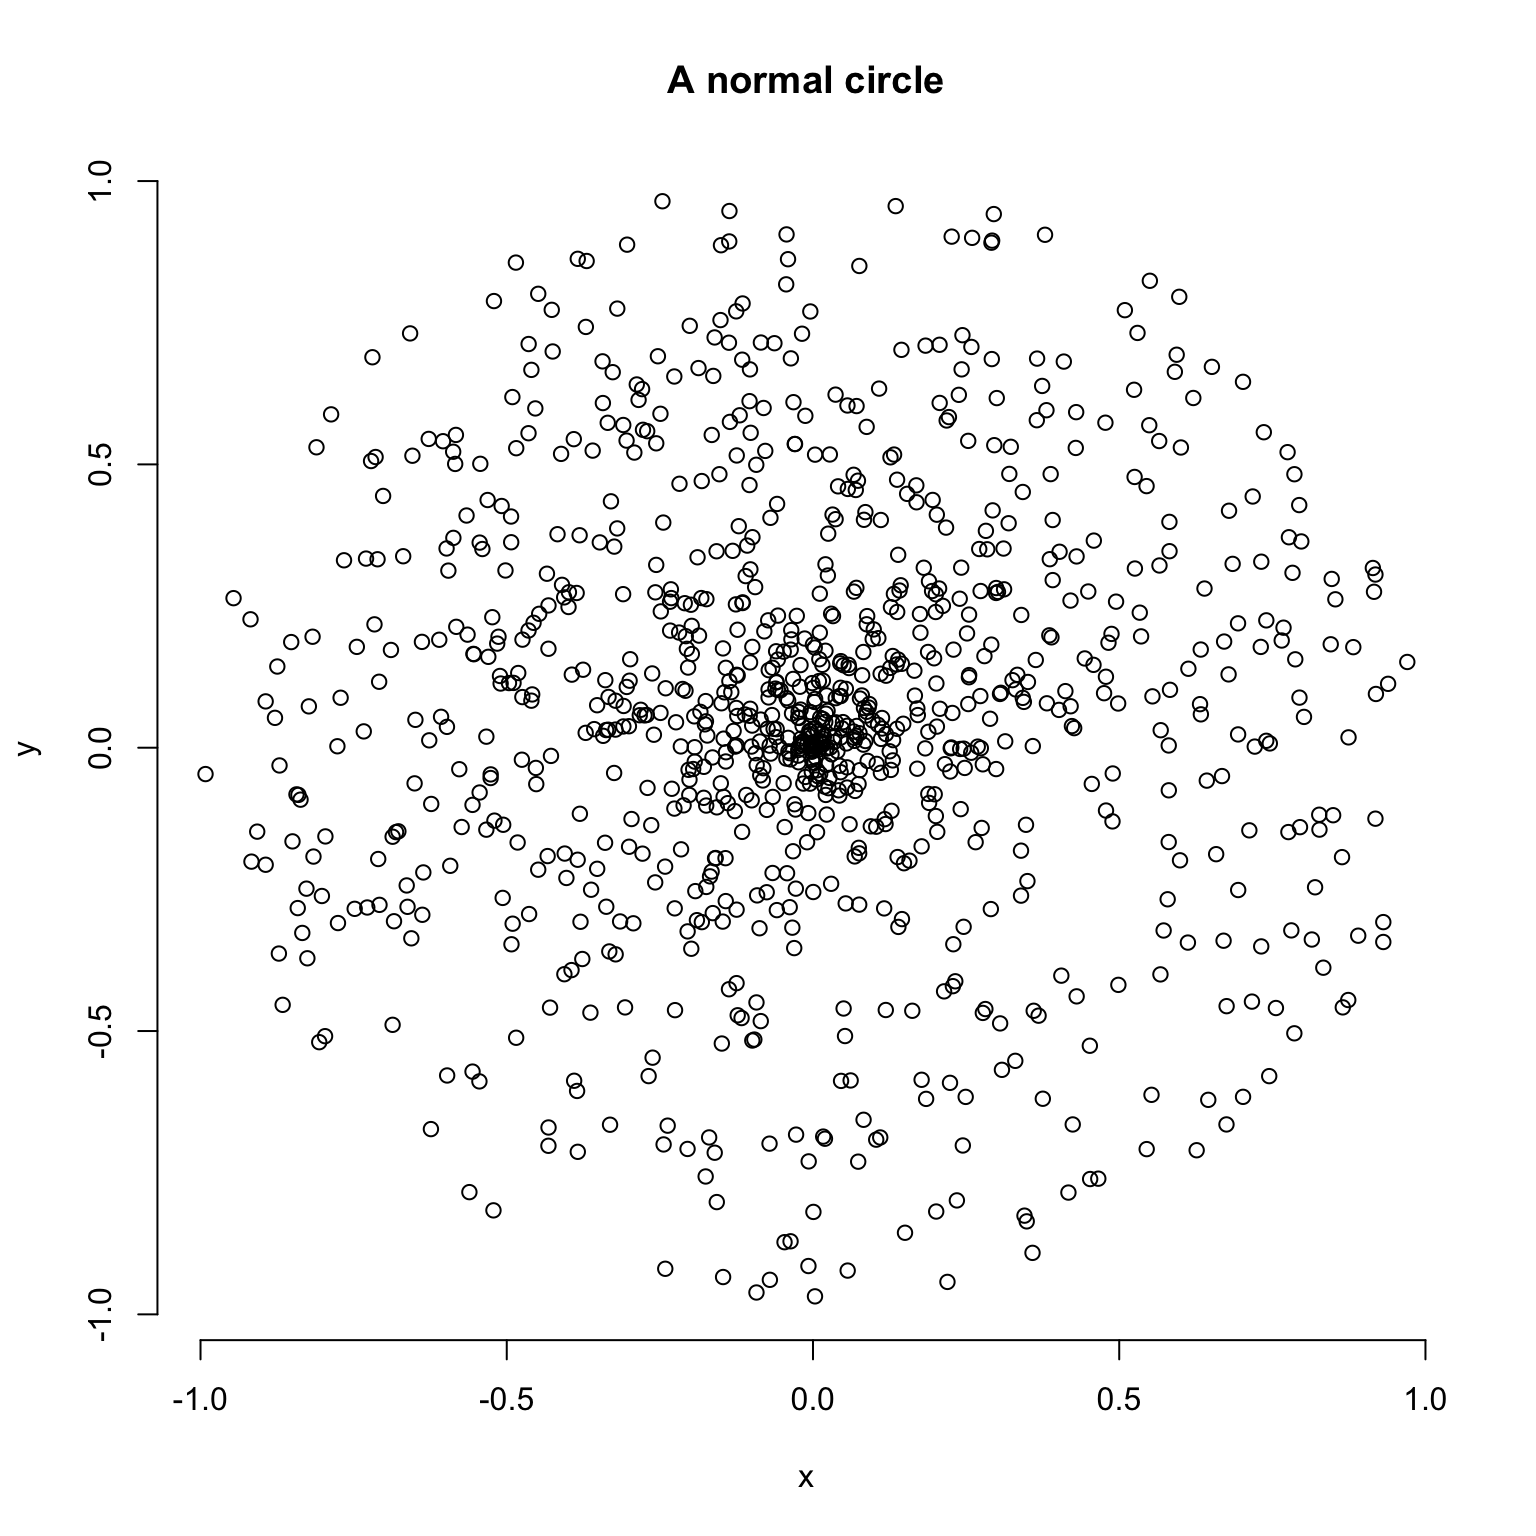
\includegraphics{dispRity_manual_files/figure-latex/unnamed-chunk-99-1.pdf}

\begin{Shaded}
\begin{Highlighting}[]
\NormalTok{## Testing against a normal distribution}
\NormalTok{disparity_normal <-}\StringTok{ }\KeywordTok{null.test}\NormalTok{(petal_disparity, }\DataTypeTok{replicates =} \DecValTok{200}\NormalTok{,}
    \DataTypeTok{null.distrib =}\NormalTok{ rnorm, }\DataTypeTok{scale =} \OtherTok{TRUE}\NormalTok{)}
\KeywordTok{plot}\NormalTok{(disparity_normal)}
\end{Highlighting}
\end{Shaded}

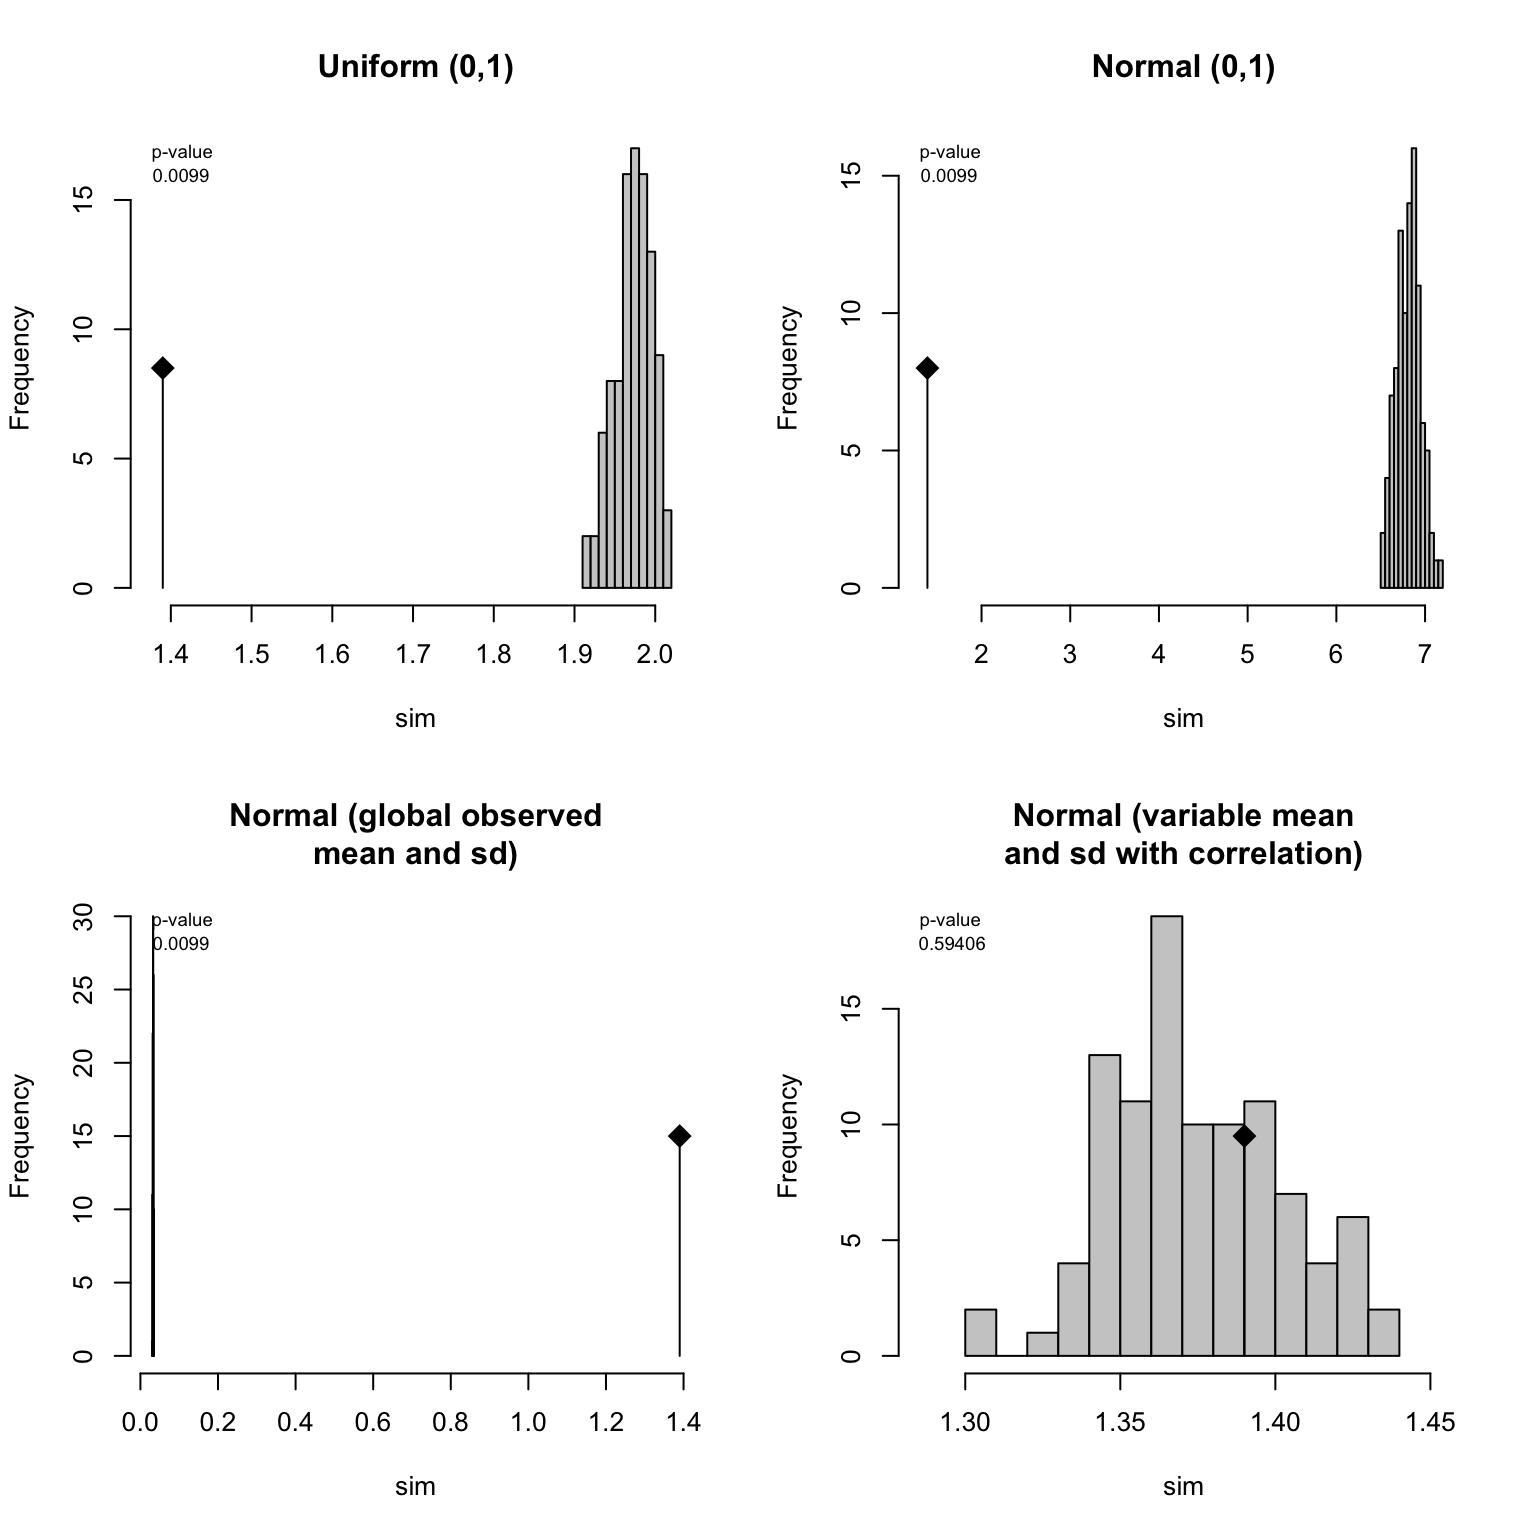
\includegraphics{dispRity_manual_files/figure-latex/unnamed-chunk-100-1.pdf}

In both cases we can see that our petal-space is not entirely normal or
uniform. This is expected because of the simplicity of these parameters.

\chapter{Future directions}\label{future-directions}

\section{More tests!}\label{more-tests}

Some more tests are being developed such as a \texttt{sequential.test}
to run sequential linear models for testing hypothesis in disparity
through time or a \texttt{model.test} developed in collaboration with
\href{https://puttickbiology.wordpress.com/}{Mark Puttick} to fit modes
of evolution to disparity curves. Stay tuned!

\section{Faster disparity
calculations}\label{faster-disparity-calculations}

I am slowly implementing parallel disparity calculation as well as C
implementations of some disparity metrics to increase significantly
improve the speed of the \texttt{dispRity} function.

\section{More modularity}\label{more-modularity}

I am equally slowly developing functions to allow more of the options in
the package to be modular (in the same way as the \texttt{metric}
argument in \texttt{dispRity}). The next arguments to benefit this
increased modularity will be \texttt{time.subsamples}'s \texttt{model}
argument and \texttt{boot.matrix}'s \texttt{type} argument.

\chapter{References}\label{references}

\begin{itemize}
\tightlist
\item
  Beck, R. M., \& Lee, M. S. (2014). Ancient dates or accelerated rates?
  Morphological clocks and the antiquity of placental mammals.
  Proceedings of the Royal Society of London B: Biological Sciences,
  281(1793), 20141278.
\item
  Cooper, N., \& Guillerme, T. (in prep.). Coming soonish!.
\item
  Diaz, S., Kattge, J., Cornelissen, J.H., Wright, I.J., Lavorel, S.,
  Dray, S., Reu, B., Kleyer, M., Wirth, C., Prentice, I.C. and Garnier,
  E. (2016). The global spectrum of plant form and function. Nature,
  529(7585), 167.
\item
  Donohue, I., Petchey, O.L., Montoya, J.M., Jackson, A.L., McNally, L.,
  Viana, M., Healy, K., Lurgi, M., O'Connor, N.E. and Emmerson, M.C,
  (2013). On the dimensionality of ecological stability. Ecology
  letters, 16(4), 421-429.
\item
  Wills, M. A., Briggs, D. E., \& Fortey, R. A. (1994). Disparity as an
  evolutionary index: a comparison of Cambrian and Recent arthropods.
  Paleobiology, 20(2), 93-130.
\end{itemize}

\bibliography{References.bib}


\end{document}
